%\documentclass{article}
\documentclass[10pt]{article}
\usepackage{times}
%\usepackage{natbib}
%\usepackage{multicol}
\RequirePackage{natbib}
\usepackage[colorlinks=true, citecolor=blue, linkcolor=blue]{hyperref}
\usepackage{amsmath, amssymb, fullpage, amsthm, array,,graphicx,asa, url}
%\usepackage[dvips]{graphics}

%\usepackage{hyperref} % for hyper reference

\graphicspath{{images/}}

% \usepackage{pifont} % this package is used to print check mark \checkmark
% \linespread{1.6} % factor 1.6 = double space

%\usepackage{setspace}
%\doublespacing


\usepackage{color}
\newcommand{\hh}[1]{{\color{magenta} #1}}
\newcommand{\dc}[1]{{\color{green} #1}}

\setlength{\oddsidemargin}{0in}
\setlength{\evensidemargin}{0in}
\setlength{\textwidth}{6.5in}
\setlength{\topmargin}{-0.4in}
\setlength{\textheight}{9in}
\evensidemargin 
\oddsidemargin

\newtheorem{thm}{Theorem}[section]
\newtheorem{dfn}{Definition}[section]
\newtheorem{cor}{Corollary}[thm]
\newtheorem{con}{Conjecture}[thm]
\newtheorem{lemma}[thm]{Lemma}

%\topmargin -0.10in   % when making pdf
%\textheight 9.15in  % when making pdf

\pdfminorversion=4 % as instructed by JASA file upload


\begin{document}

\tableofcontents

% Article top matter
\title{Human Factors Influencing Visual Statistical Inference }
\author{{Mahbubul Majumder, Heike Hofmann, Dianne Cook}
\thanks{Mahbubul Majumder is a PhD student (e-mail: mahbub72@gmail.com), Heike Hofmann is an Associate  Professor and Dianne Cook is a Professor in the Department of Statistics and Statistical Laboratory, Iowa State University, Ames, IA 50011-1210. This research is supported in part by the National Science Foundation Grant \# DMS 1007697.}}
\date{\vspace{-.5in}}
%\date{\today}  %\today is replaced with the current date
\maketitle

\begin {abstract}  
Visual statistical inference is a way to determine significance of patterns found while exploring data. It is dependent on the evaluation of a lineup, of a data plot among a sample of null plots, by human observers. Each individual is different in their cognitive psychology and judiciousness, which can affect the visual inference. The usual way to estimate the effectiveness of a statistical test is its power. The estimate of power of a lineup can be controlled by combining evaluations from multiple observers. Factors that may also affect the power of visual inference are the observers' demographics, visual skills, and experience, the sample of null plots taken from the null distribution, the position of the data plot in the lineup, and the signal strength in the data. This paper examines these factors. Results from multiple visual inference studies using Amazon's Mechanical Turk are examined to provide an assessment of these. The experiments suggest that individual skills vary substantially,  but demographics do not have a huge effect on performance. There is evidence that a learning effect exists but only in that observers get faster with repeated evaluations, but not more often correct. The placement of data plot in the lineup does not affect the inference.

{\bf Keywords: \sf statistical graphics, non-parametric test, cognitive phycology, data visualization, exploratory data analysis, data mining, visual analytics.} 
\end {abstract}

%\begin{multicols}{2}
%\twocolumn

\section{Introduction}  

The lineup protocol introduced in \citet{buja:2009} can be used to test the significance of findings during the exploratory data analysis. The methodology is a part of what is called visual statistical inference.  These concepts have been developed further by \citet{majumder:2013} who refined the terminology and validated the lineup protocol with a head to head comparison with conventional inference. One of the major contributions of  \citet{majumder:2013}  is to define the power of the visual test and provide methods to obtain the power for a particular lineup. It was observed that the power can be as good or better than that of a conventional test in some scenarios.

In visual inference, the test statistic is a plot of the observed data. To create a lineup, this plot, called the actual data plot, is placed in a layout of null plots. The null plots  are generated from the model specified by a null hypothesis, essentially describing what the plot might look like if the data had no structure. An observer is asked to evaluate the lineup. If the  actual data plot is detected by the observer, the null hypothesis is rejected. This means that the structure in the actual data plot has significant structure, a pattern that is not simply due to randomness. Combining the choices of multiple observers provides more stability in the estimation of significance.

%\subsection{Visual inference example}


\begin{figure}[hbtp] 
   \centering
   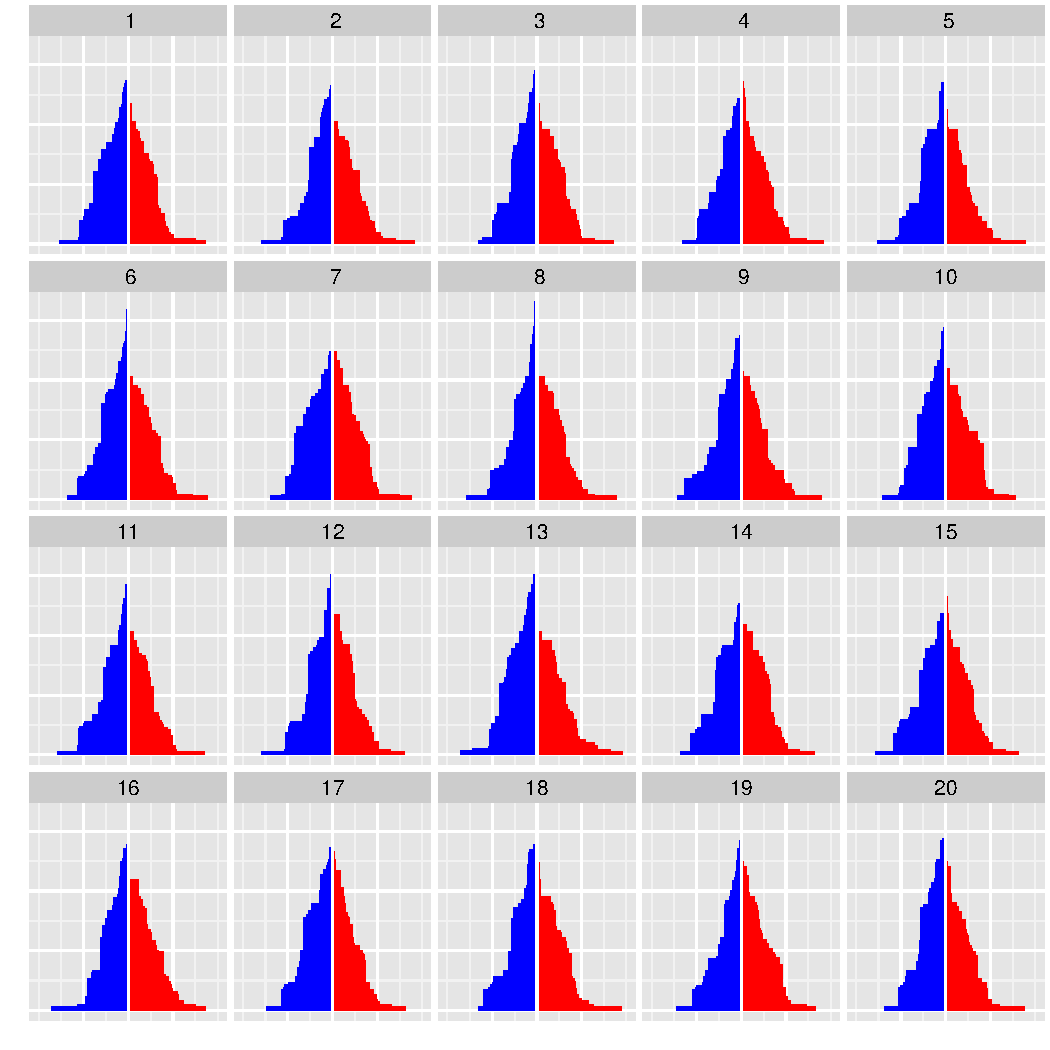
\includegraphics[width=0.99\textwidth]{electoral-5-13.pdf} 
%      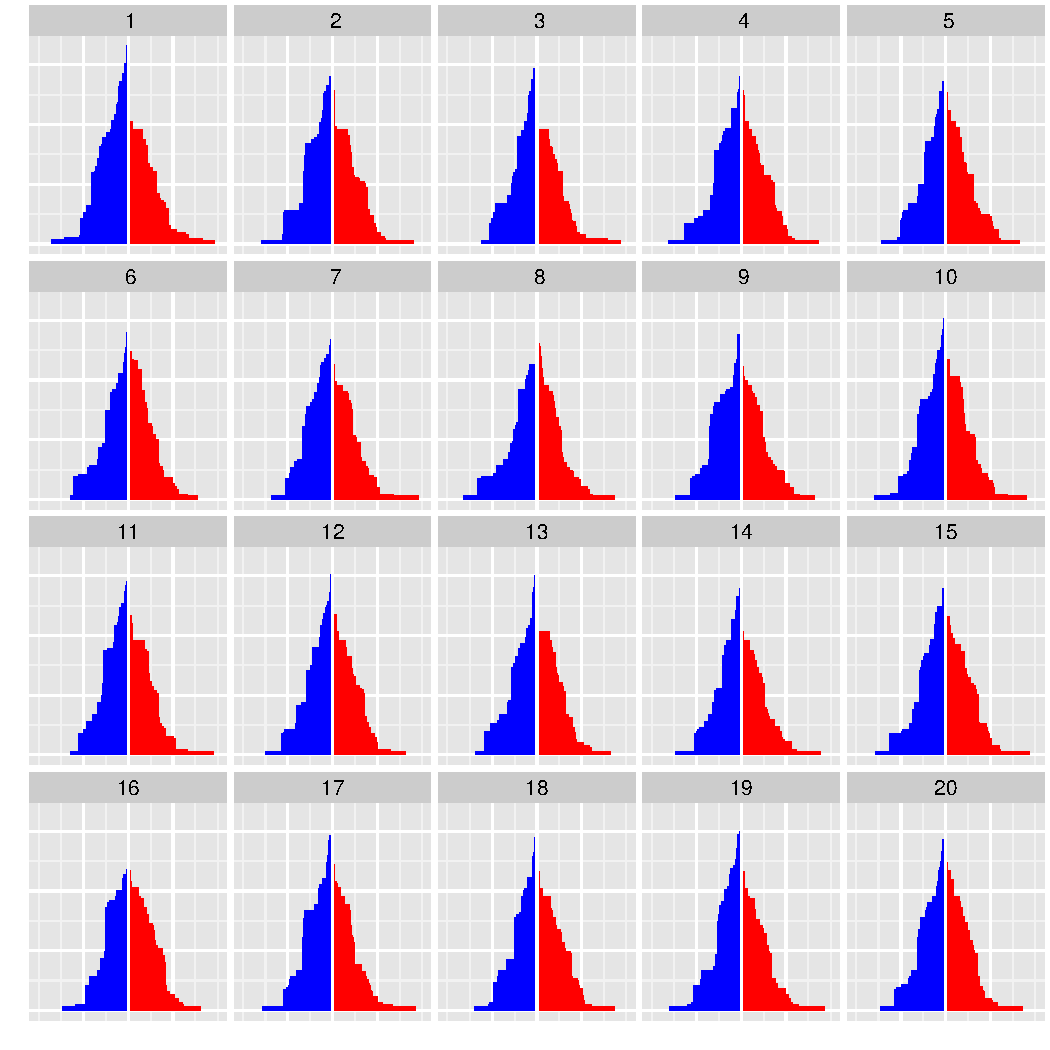
\includegraphics[width=0.99\textwidth]{electoral-1-1.pdf} 
   \caption{ \label{fig:elect-1} Which one of the plots is the most different from the others?}
\end{figure}

Figure~\ref{fig:tower} displays a lineup of 20 plots where one of the plots is observed data, while the remaining 19 plots are rendered from data generated under a null model. Which one of the 20 plots is the most different from the others? When asked this question, 12 of 72 observers picked the same plot (with number equal to the result of $3^2+4$), with reasons given being 'asymmetry' (36\%), 'trend' (26\%) or `outliers' (16\%).  The corresponding $p$-value is 0.00023, indicating sufficient evidence to reject the null hypothesis. 

What does this mean, though? For that, we need to know the context of the data and we need to have more information about the generation of the null plots. For that, we need to know the context of the data and we need to have more information about the generation of the null plots. This example investigates the results from the 2012 US presidential election in comparison to the poll results just prior to the election. 
(Although this example is more simplistic than most of the tests conducted to date, it will serve the purpose of illustrating the lineup protocol.) The data is looking at the difference in poll results between the two (major) presidential candidates, Obama and Romney, for all states. Each panel in Figure~\ref{fig:elect-1} shows an `electoral building' where each state in the union is represented by a rectangle. This difference is plotted horizontally, and the height of each box corresponds to the state's electoral votes. Color indicates party affiliation.  The null hypothesis is ``that the election results were consistent with the polls''. The polling results provides the null model from which data is simulated. Because each poll has a margin of error, this is used to simulate different scenarios that might have resulted on election day, if the polls were on target. A null data set is generated as a set of draws from normal distribution, with mean equal to the difference in poll percentage of the latest state poll results, and standard deviation equal to 2.5, approximating a margin of error of 5\%. These samples are plotted as electoral buildings, and the plot made with the results from the election is placed randomly among them in a lineup of size $5\times 4$. If the null hypothesis is true the actual data plot should look just like any of the other plots, and not be identified by an observer. Figure~\ref{fig:tower} shows a plot of the electoral building with added context information and labels.
 %A party needs 270 electoral votes or more to win the presidential election. 
%\begin{figure}[htbp] 
%   \centering
%   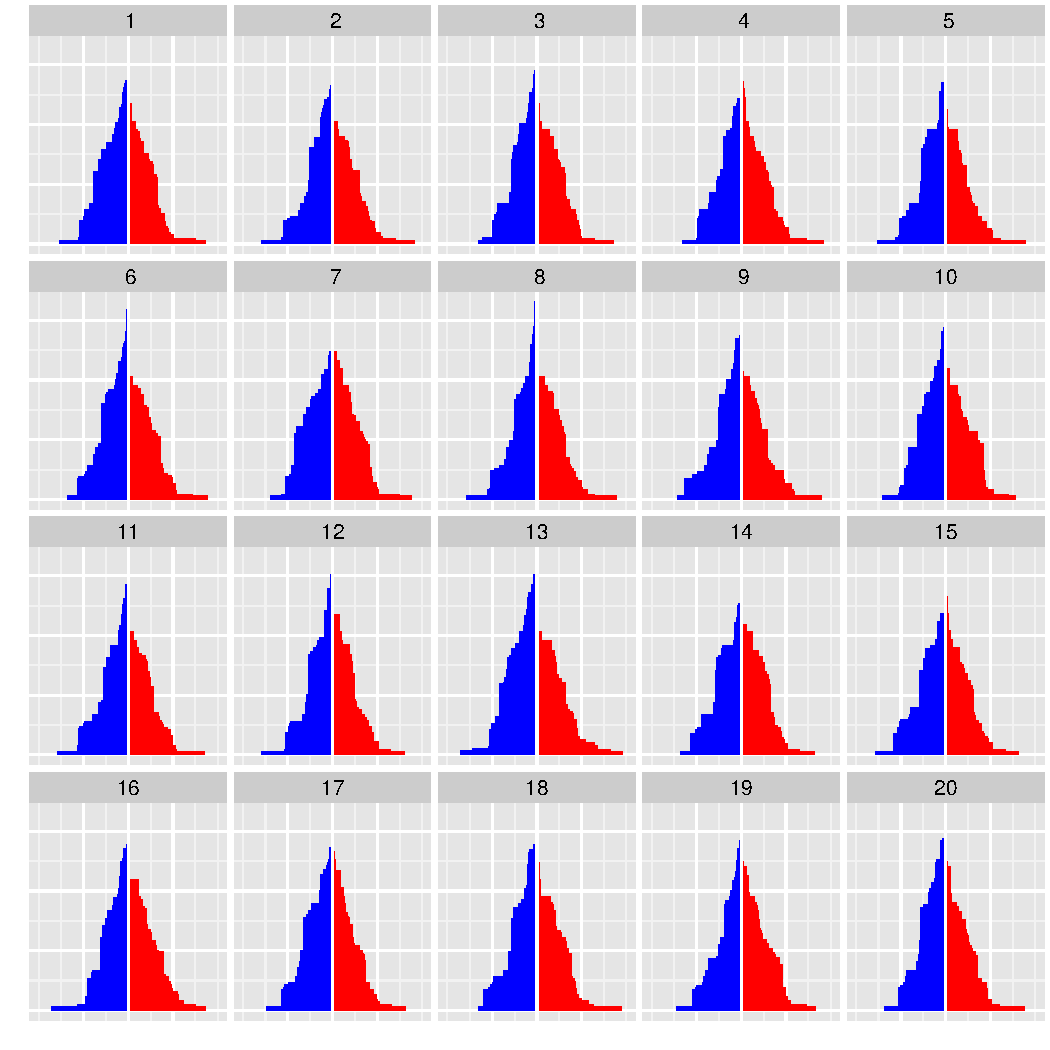
\includegraphics[width=0.8\linewidth]{electoral-5-13.pdf} 
%   \caption{Which plot looks the most different from the other plots?  Lineup \#1 - electoral building; another set of four lineups can be found in figs.~{fig:elect.2} through~{fig:elect.5}}
%   \label{fig:elect.1}
%\end{figure}


\begin{figure}[hbtp] 
   \centering
   \begin{minipage}[c]{0.49\textwidth}
   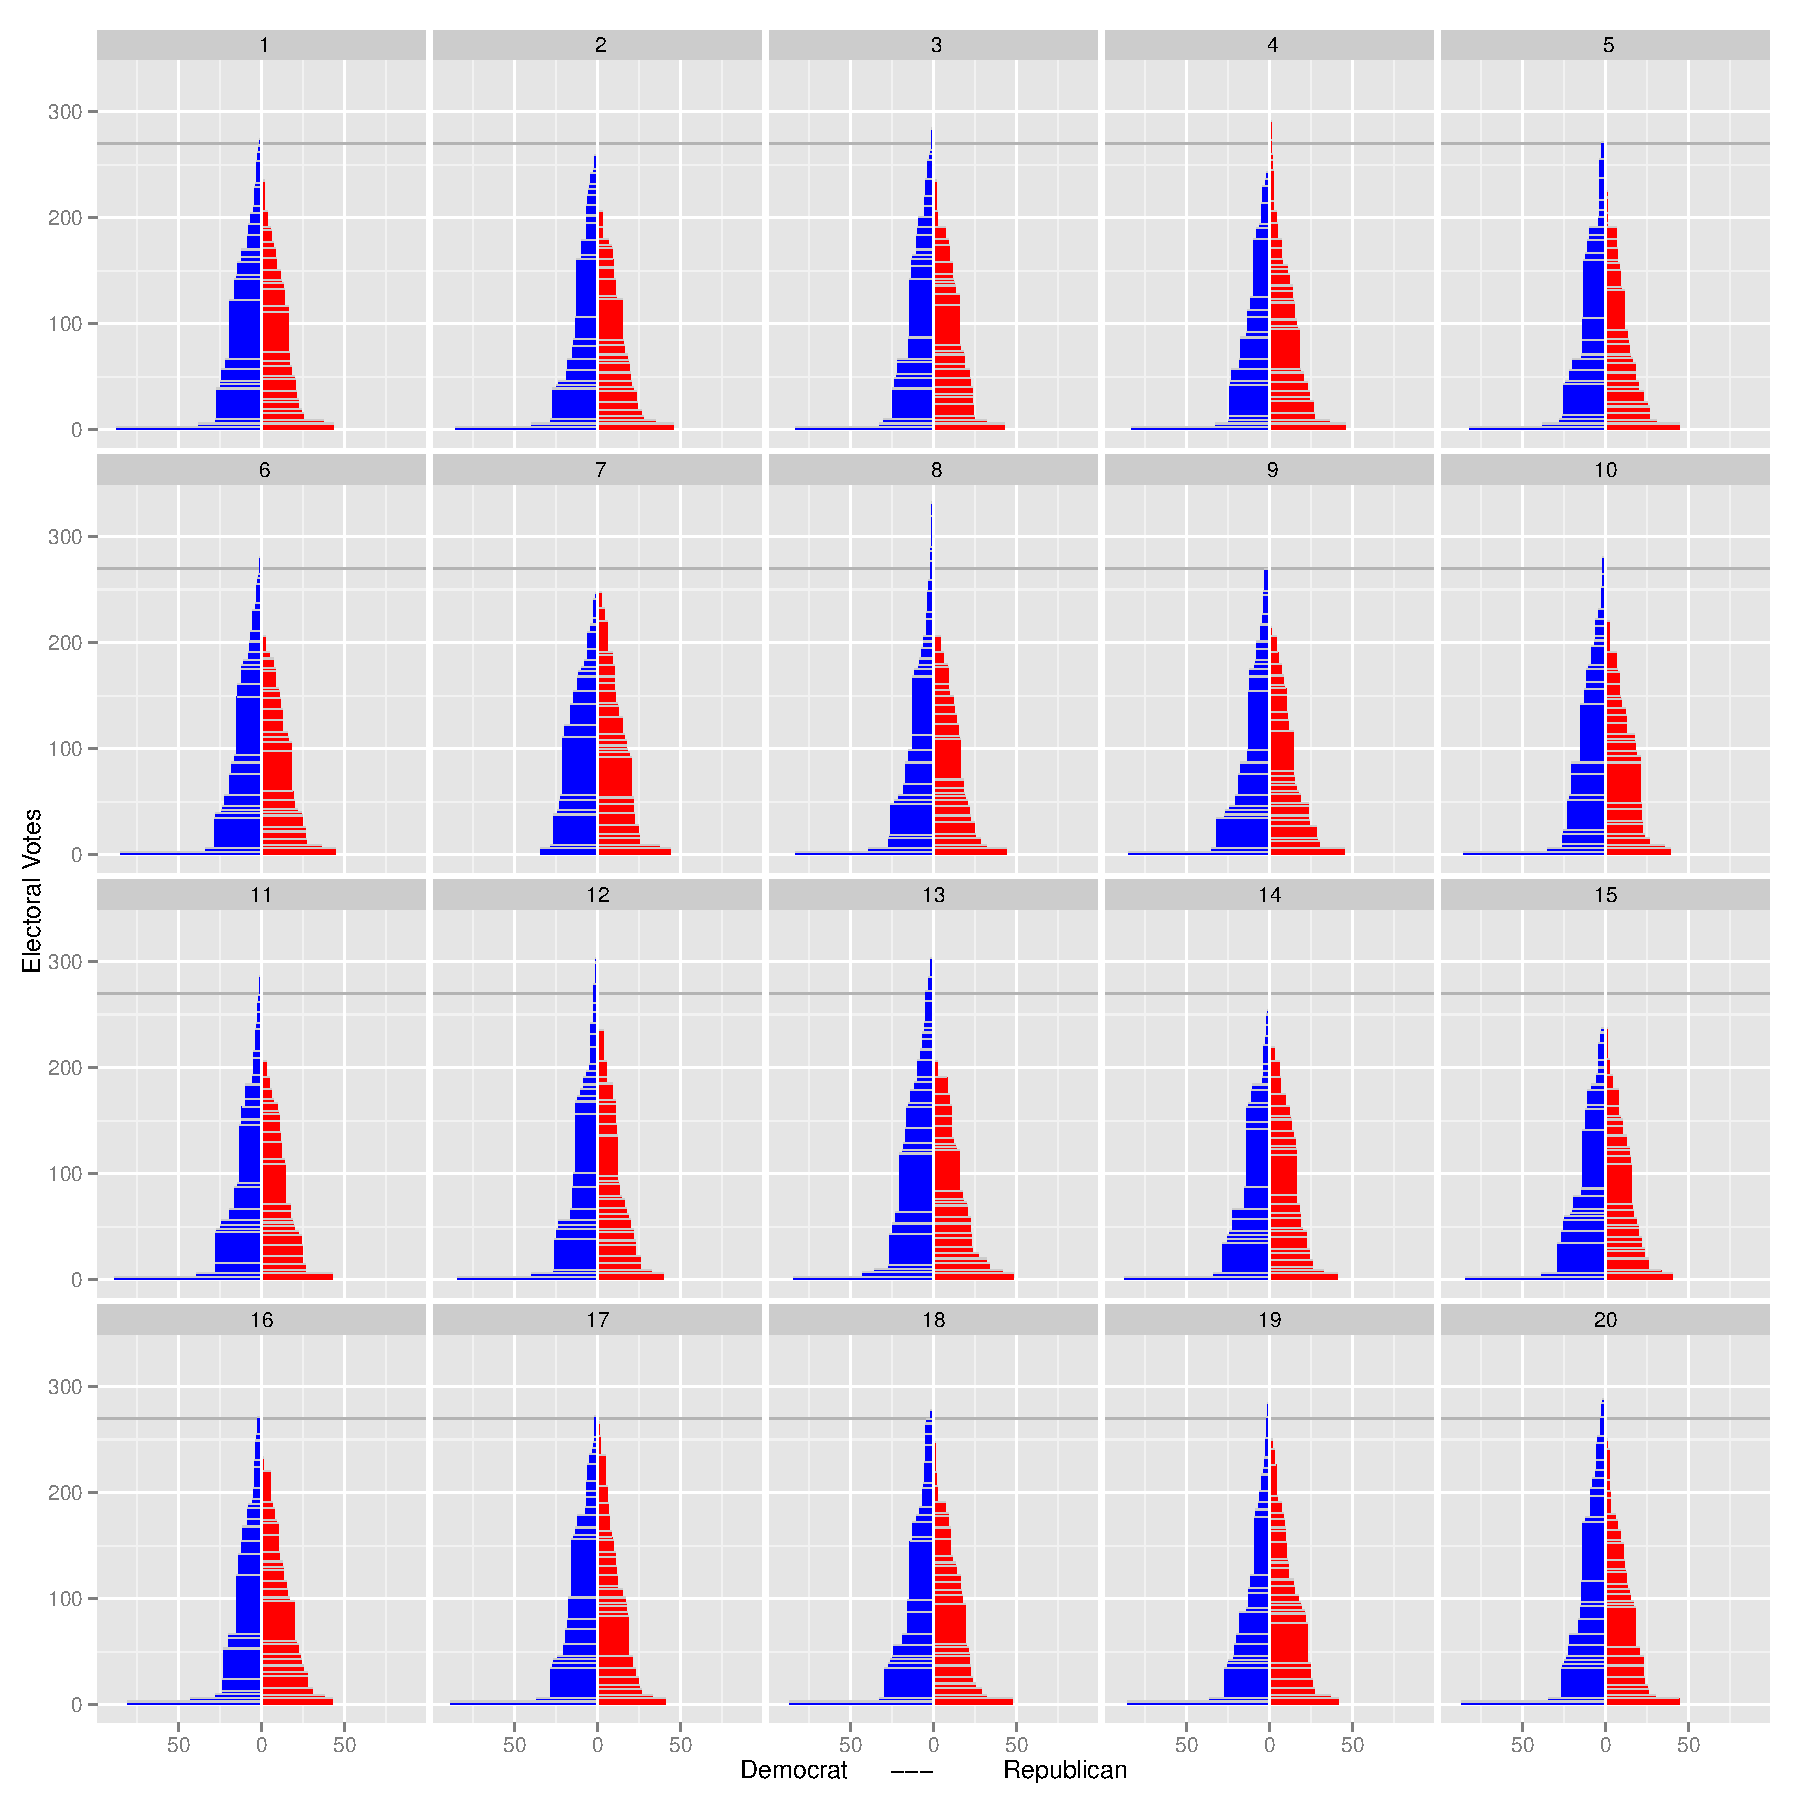
\includegraphics[width=\textwidth]{tower.pdf}
   \end{minipage}
    \hfill
   \begin{minipage}[c]{0.45\textwidth}
   Poll aggregator 1 \\
      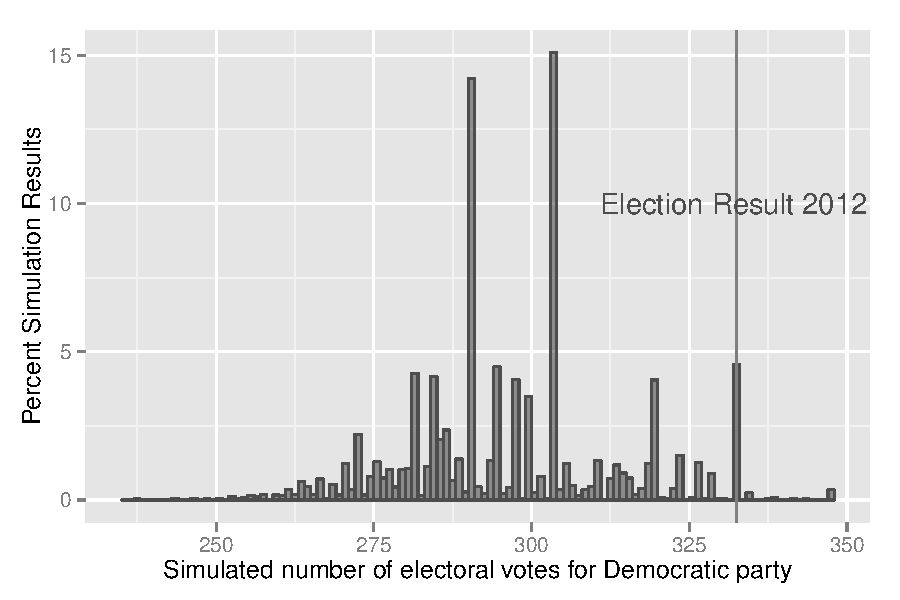
\includegraphics[width=\textwidth]{freedom-sim.pdf} 
   Poll aggregator 2\\
      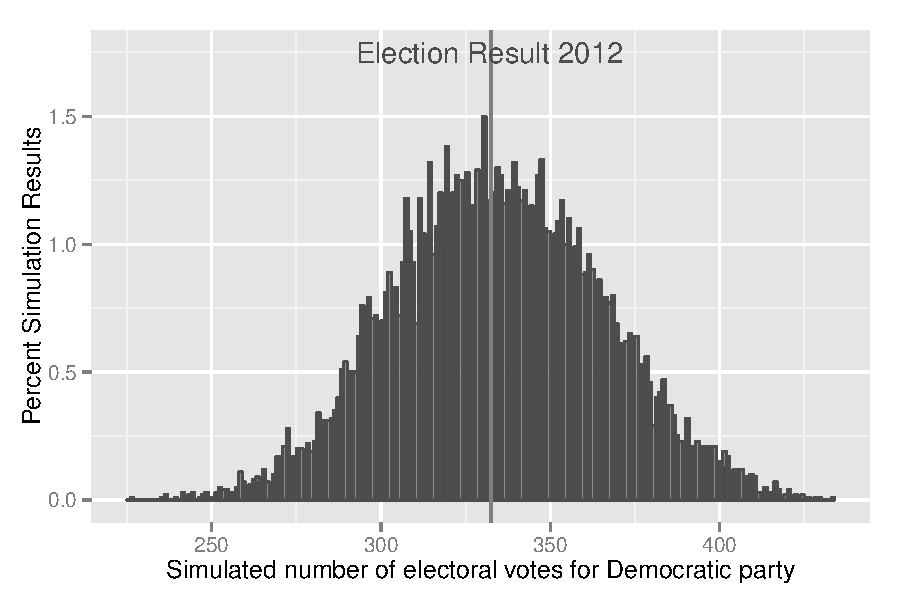
\includegraphics[width=\textwidth]{rcp-sim.pdf} 
   \end{minipage}
   \caption{ \label{fig:tower} Electoral building plot of the results of the 2012 U.S. Presidential Election (left). On the right two histograms of 10,000 simulations each based on polling averages from two different sources. For the histogram on the top, the $p$-value of observing results as extreme as  the  2012 U.S. election results based on the bootstrap is 0.0533 (with Bootstrap standard error of 0.002), making the election results almost significantly different from the polls (data source for poll aggregator 1 is Freedom`s Lighthouse Averages). There is no indication of any inconsistency between polls and election results based on the bootstrap simulation below (data source for poll aggregator 2 is RealClearPolitics Averages). The lineups are based on the top source.}
\end{figure}

%The rest of the 19 plots are generated from the assumption that there is no difference between two groups of data. For this, the group structure of the data is broken by random permutation of the groups. 

%If the null hypothesis is true, the observed data should look similar to the rest of the plots in the lineup making it difficult to detect the observed plot. On the other hand, if the null hypothesis is not true, the observed data should be different from the rest of the plots in the lineup and observers should be able to pick the data plot out from the rest.


A lineup can be evaluated by a single person or multiple observers. A binomial distribution is used to calculate the $p$-value based on the number of times observers identify the actual data plot, which provides the information needed to make a decision on rejecting or failing to reject the null hypothesis.  Observers should not be aware of the data that constitutes a lineup, and should not have seen the actual data plot before seeing the lineup. This is the reason that in the election example, above, the scenario was explained after the lineup question, in the text. 

The question that is asked of the observer should be as general as possible, effectively asking the observer to pick the plot that is different, and allowing them to provide their reasons for seeing their pick as different. In some of the studies, the ones described in  \cite{majumder:2013} very specific questions were asked, because the experiments were being conducted to compare results from the lineup protocol with those of conventional tests. In those experiments, structure in the data was strictly controlled in the simulation process, which allowed for specific questions to be asked. In the election example, observers were asked ``which plot is the most different?''. The type of plot, showing two (modified) stacked bar charts in different colors should suggest to the observer that the interesting feature is most difference between the two heights. Most observers got this, but it is possible that some observers might pick plot 4, where the red tower is slightly above the blue as the most different because it is the only plot with this feature. So a better question may have been ``Which plot shows the biggest height difference between the two towers?'' except that this tailors the inference to a specific feature which does not match the null hypothesis of interest. 
%=======
%A lineup can be evaluated by a single person or multiple observers. Based on the feedback of $K$ observers a $p$-value is computed with the help of a binomial random variable $X$ for the number of observers picking the data plot. Under the null hypothesis is $X$ is  distributed according to $B_{K, 1/20}$ \citep{majumder:2013}. The $p$-value for a lineup is then given as $P(X \ge x)$. 
%%This finally a decision is made about the hypothesis being tested.
%>>>>>>> example

%\begin{figure}[htbp] 
%   \centering
%   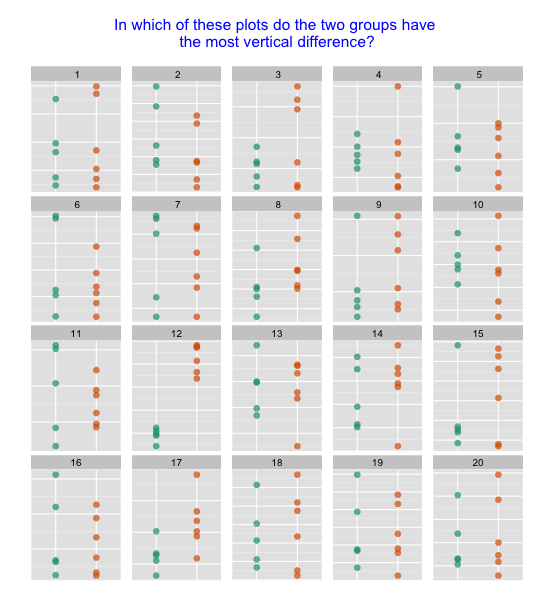
\includegraphics[width=6.5in]{plot_turk9_geno_4_3.png} 
%   \caption{A lineup of 20 plots. One of the plots is observed data and rest of the 19 plots are obtained by randomly permuting the group structure. Can you identify the observed data?}
%   \label{fig:lineup_geno}
%\end{figure}

%\subsection{Observer task}

For any evaluation the observer may or may not identify the actual data plot. Under the null hypothesis, the actual data plot should look similar to the null plots making it harder to detect. It is not expected that an observer would be able to detect the data plot in this scenario. But since there are limited number of plots in a lineup, which is 20 in the election example, there is a 1/20 chance that the observer would pick the actual plot. This proportion is associated with the Type~I error of the test. On the other hand, if null hypothesis is not true, the observed plot should look different from the null plots, making it easier to be detected. This is the definition of the power of the test. When multiple observers evaluate a lineup, the proportion of correct response can be used to estimate the power. The ability of individual observers can vary, and examining this is the purpose of this paper.

%For a lineup with fixed difficulty, the proportion correct responses may vary for different observers. If an observer evaluates multiple lineups, the proportion of correct evaluations by the observer could be used as a measure of performance by an observer. The another way of measuring the performance of the observer could be the time taken by an observer to evaluate a lineup. Since performance would also depend on the lineup difficulty it is essential to adjust for lineup difficulty before estimating the performance of the observer.

%Some of the factors that may affect the performance of the observer are discussed in Section \ref{sec:factor_performance}. In this paper we focus on estimating the learning effect of the observer in terms of both proportion correct and time taken to evaluate a lineup through the attempts made during the evaluation of multiple plots. We also estimate the location effect of the observed data plot in a lineup. The other factors are controlled in simulation experiments so that learning effect and location effect can be estimated.

\begin{table*}[hbtp] 
\centering 
\caption{Overview of 10 different Turk experiments, from where data was taken to study human factor effects. All of the experimental data was used to estimate the effect of demographic factors (DF) on visual inference while three were suitable for assessing learning trend (LT) and location effect (LE) was possible to assess using just one specially designed study.} 
\begin{tabular}{m{.5cm}m{2.6cm}m{2cm}m{5.5cm}m{3cm}} 
\hline\hline 
 & Experiment &  Test Statistic  & Lineup question & Used in study of\\ [0.5ex] % inserts table %heading 
\hline 
1  & Box plot & \begin{minipage}[t]{2cm} \begin{center}	\scalebox{0.12}{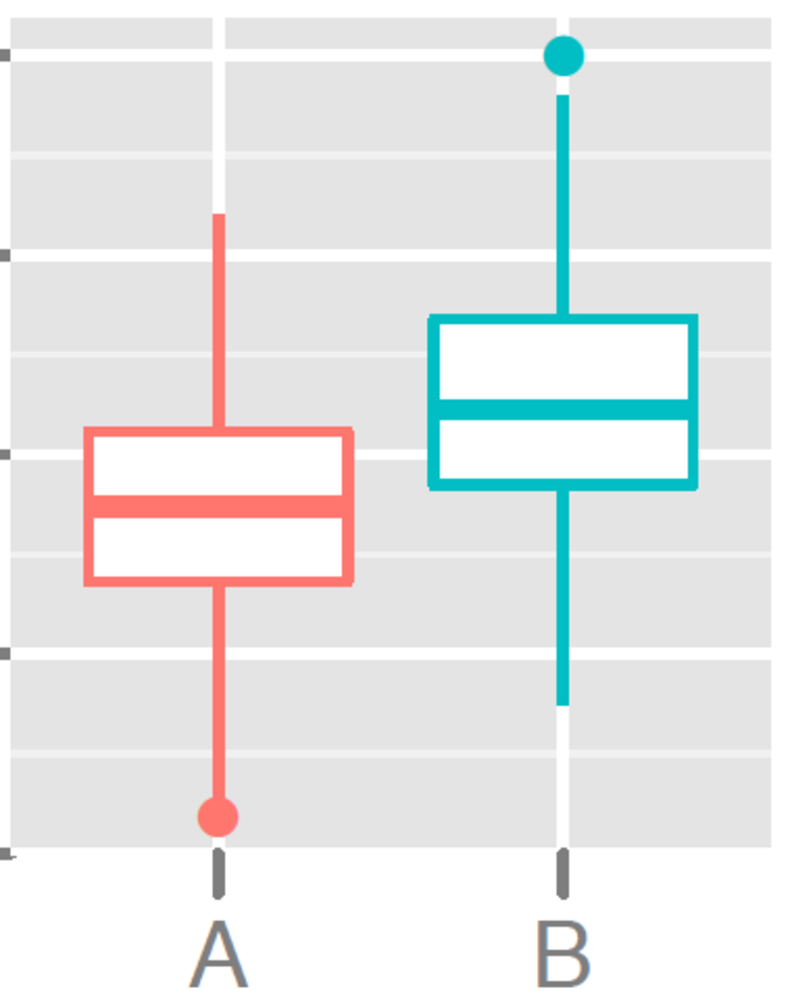
\includegraphics{stat_category1.pdf}} \end{center} \end{minipage} & Which set of box plots shows biggest vertical difference 
between group A and B? & DF\\
2 &  Scatter plot & \begin{minipage}[t]{2cm}  \begin{center} \scalebox{0.3}{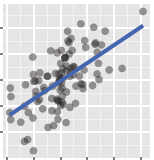
\includegraphics{stat_beta_k1.png}} \end{center} \end{minipage} & Of the scatter plots below which one shows data that has steepest slope? & DF\\
  3 & Contaminated plot &\begin{minipage}[t]{2cm} \begin{center} \scalebox{0.5}{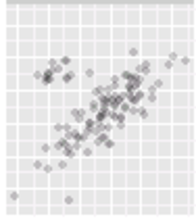
\includegraphics{stat_contaminated.pdf}} \end{center} \end{minipage} & Of the scatter plots below which one shows data that has steepest slope? & DF\\
 4 & Polar vs Cartesian & \begin{minipage}[t]{2cm} \begin{center}  \scalebox{0.32}{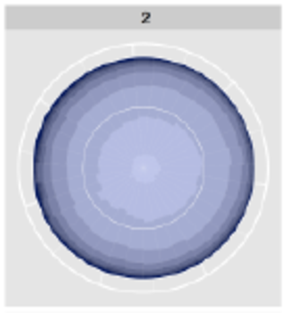
\includegraphics{stat_polar.pdf}} \end{center} \end{minipage} &Which plot is different?& DF\\
  5 & Hist vs density & \begin{minipage}[t]{2cm} \begin{center}  \scalebox{0.38}{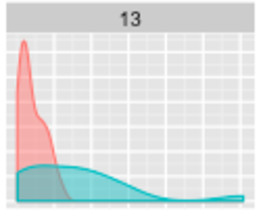
\includegraphics{stat_density.pdf}} \end{center} \end{minipage} &In which plot is the blue group furthest to the right?&  DF and LT \\  
  6 & Violin vs boxplot & \begin{minipage}[t]{2cm} \begin{center}  \scalebox{0.35}{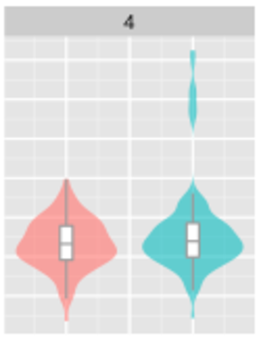
\includegraphics{stat_violin.pdf}} \end{center} \end{minipage}&  In which plot does the blue group look the most different from  the red group? &  DF and LT \\
  7 & Group separation & \begin{minipage}[t]{2cm} \begin{center}  \scalebox{0.4}{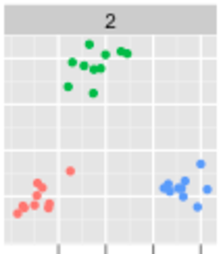
\includegraphics{stat_separation.pdf}} \end{center} \end{minipage} &Which of these plots has the most separation between the coloured groups? & DF and LT \\ 
  8 & Sine Illusion & \begin{minipage}[t]{2cm} \begin{center}  \scalebox{0.28}{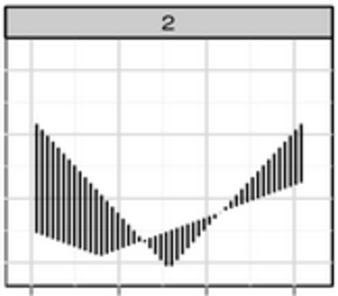
\includegraphics{stat_sine.pdf}} \end{center} \end{minipage} & In what picture is the size of the curve most consistent? & DF\\ 
  9 & Gene expression &\begin{minipage}[t]{2cm} \begin{center}  \scalebox{0.45}{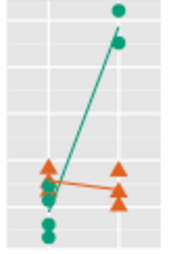
\includegraphics{stat_gene.pdf}} \end{center} \end{minipage} & In which of these plots is the green line the steepest, and the spread of the green points relatively small? & DF and LE\\ 
  10 & Test normality & \begin{minipage}[t]{2cm} \begin{center}  \scalebox{0.35}{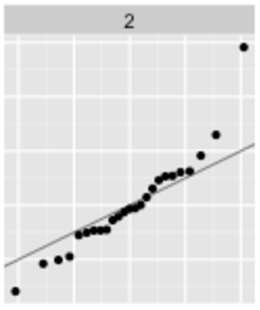
\includegraphics{stat_normality.pdf}} \end{center} \end{minipage} &Which of these plots is most different from the others? & DF\\ 

\hline 
\end{tabular} 
\label{tbl:visual_stat} 
\end{table*} 

There have been ten experiments conducted using Amazon's Mechanical Turk~\citep{turk} that are being used to evaluate the effects of observers' demographic factors on the inference. Table \ref{tbl:visual_stat} summarizes these experiments. Each of these experiments collected demographic details of the subjects. Experiments 5, 6 and 7 are used to study the learning trend of the observer. The design of experiment 9 incorporated components that allows position of the actual data plot in the lineup, and the sample of nulls, to be evaluated. Section \ref{sec:factor_performance} discusses human factors that may affect the performance of the observer. Section \ref{sec:exp_design} describes the methods used to assess the effects, and Section \ref{sec:result_socio} describes the results.

%\subsection{Experiments pooled}



\section{Factors Potentially Affecting Visual Inference} \label{sec:factor_performance} 

Because visual statistical inference relies on plotting choices, lineup design and human evaluation, it is important to understand how these factors that might affect results.  This section provides a brief description of the factors that are expected to have some impact on the performance of visual statistical inference.  

%ased on human evaluation on a lineup a decision is made in visual statistical inference. While the visual test statistic is defined to have a direct influence on the observer to pick a plot based on the signal in the data, there are other human factors that may affect the observer performance. It is important to study the effect of those factors and examine the extent of their influence. This section presents a brief description of the factors that may affect the power of visual inference.   

%\dc{You need to have more than one sentence to open this section, it needs a paragraph overviewing the factors.}

\subsection{Choice of Visual Test Statistic}  

There are a variety of ways that data can be plotted and enhanced. The choice of plot that is used as the visual test statistic should be closely associated with the problem being investigated. For example, side-by-side boxplots may be more appropriate than side-by-side dotplots, when one variable is categorical. Enhancements, such as a line overlaying a scatterplot to represent a fitted model, might be appropriate for studying some types of problems.  Some choices of visual test statistics provide better results than others when studying the same problem, which is discussed in \cite{heike:2012}.  This makes sense, because some plot types will make it easier for see some structure. It also presents as a flip-side to visual inference, that the same methods could be used to determine the optimal plot choice. 

Table \ref{tbl:visual_stat} shows the visual test statistics used in the Turk studies completed so far. Side-by-side boxplots were used in experiment 1 to study the importance of a categorical variable in a regression model. For both experiments 2 and 3 a scatterplot is used but a regression line fitted through the points is overlaid for experiment 2. It is easier to spot the slope of the line compared to just the scatterplot itself. But people are better in noticing the unusual pattern in the data which is some contamination purposefully added for experiment 3. Experiment 4 compared polar coordinates to euclidean coordinates on the reading of structure in a barchart.  In addition, this experiment also examined the style of plot for a bivariate data problem: a scatterplot, side-by-side dot plots, overlaid densities or side-by-side boxplots. .... expand description of experiments here...

\subsection{Signal in the Data}

The visual test statistic is chosen so that it displays a specific pattern in case the null hypothesis is not true. Thus the most important factor that help an observer to correctly evaluate a lineup is the presence of any detectable signal in the data. On the other hand, if the null hypothesis is not true, visual test statistic should not display any distinguishable pattern. In fact, some of the null plots may appear to be the most different plot in a lineup influencing the observer to chose a plot different than actual data plot. This is an elegant feature of the lineup. It force the observer to chose a wrong plot when the null hypothesis should not be rejected.

%Plots to do: for the same signal strength show the proportion correct for scatterplot and boxplot. eg., qplot(effect, ump-visual power, color= plot-type)

\subsection{Question that Human Observer Answers} The researcher knows about the underlying hypothesis but the observer does not necessarily know the underlying details of the lineup. So, the researcher needs to ask a question to the observer to answer while evaluating the lineup. This question should provide the observer a little clue so that the answer reflects the hypothesized patterns in the actual plot. For example Table \ref{tbl:visual_stat} shows the questions asked for the simulation experiments considered for this study. Notice that for case 1 if the observer can identify the actual plot in the lineup that should indicate that the plot chosen has the most vertical difference between groups A and B which is exactly what the researchers intend to examine. Similarly for case 2, a correct evaluation would indicate that the slope is different than the slope that may show up just from randomness.

These questions are very crucial for the power of visual test. They help observer think in a meaningful direction. Notice that there may be unnecessary patterns in the actual data plot which may not necessarily indicate the existence of the significant signal in the plot. These questions help observer not to be misguided by those patterns. To follow up further on this \citet{majumder:2013} also collected reasons of choice made by the observers and noticed that Type-III error may occur where the hypothesis may be correctly rejected but for a wrong reason. 



%\subsection{Observer Personality} 

%\subsection{Visual Perception of Human Eye} Different people observe the lineup in different ways.  With the help of eye-tracking equipment \citet{zhao:2012} track the observers' eyes to see how they go through the plots in a lineup to come to their answers. The result suggest that people have particular methods of reading lineups. Some people read lineups from left to write direction while some read from upward to downward. Some people start looking from the center of the lineup while others start from the top left corner. In the earlier phase of the exercise, the observer tend to scan the plots and then start comparing plots to make a final decision. Beside right-left or up-down directions observer show some diagonal movement too. 
%
%Given this pattern of human eye tracks, it may effect the performance of an observer depending on where the actual plot is placed in the lineup. If the actual plot is on the top left corner and the observer starts from that point it may be easier to detect the actual plot earlier in the exercise and the observer could get plenty of time to make comparison. Thus the position of the actual plot in a lineup may have some impact.

\subsection{Demographics of the Observer}  Some of the demographics of the observer such as age, gender, education level and geographical location may have effect on how an observer would examine the lineup. This may produce some variability in the performance of the observer. For example, a high school student may not respond same as a well educated person while evaluating a lineup. There may be variations in different age groups as well. Investigation on subjects with a well variety of age groups is necessary to study this variability. 

To meet the Institutional Review Board (IRB) requirement, it is necessary to exclude any subject less than 18 years of old to participate human subject experiment. Thus we intend to only focus on the performance of observer with age 18 years or older. We don't expect many older people to participate our study and we are interested of age from 18 to 65 years.

Education level has some relation with age. Younger observer may not have higher degree. Thus some of the variability in performance for different education level may be confounded with age. On the other hand, it could be possible to have undergrad degree with higher age. Specially for any geographical location where not many certain gender group have higher education, this may occur. Thus the effect of all these demographical factors may be confounded at certain level. 

We don't expect much difference in performances between male and female observers. Gender may have some influence through the education level and geographical locations since some location may have small number of educated female population. We intend to include similar number of male and female subjects in our study so that this can be examined.

\subsection{Learning Trend of the Observer} When an observer evaluates a lineup he or she may learn something from the experiences of the earlier observations. If the same observer is shown another lineup the learning from previous evaluation may help. The more evaluations an observer makes the more skillful the observer may become. This learning trend may or may not be significant overall but it may influence the performance of the observer in some way. 

Learning may occur in two different ways. An observer can become more trained on the lineup structure and the pattern in the plots shown. This can be learning in proportion of correct evaluation. Or, he or she may become efficient in responding faster in the later evaluations. This can be observed as the time taken for evaluating a lineup. This paper investigates both of these learning trends with multiple simulation experiments.

When an observer evaluate a lineup for the first time, he or she has to read through many instructions and become familiar with the environment of the experiment. We expect that this will require much more time compared to the rest of the evaluations. Time taken for the second or successive attempt should be much lower than the time taken for the first lineup. We attribute this to the adaptation to the experiment environment, not a learning of evaluating a lineup.

\subsection{Location of Actual Plot in the Lineup} The actual data plot is placed in a random spot in a lineup. While evaluating the lineup some people may start looking from some specific part of the lineup. With the help of eye-tracking equipments \citet{zhao:2012} tracked the observers' eyes to see how they went through the plots in a lineup to come to their answers. The results suggest that people have particular methods of reading lineups. Some people read lineups from left to right direction while some read from upward to downward. Some people start looking from the center of the lineup while others start from the top left corner. In the earlier phase of the exercise, the observer tend to scan the plots and start comparing plots to make a final decision. Beside right-left or up-down directions observers show some diagonal movement too. 

Given a specific pattern of eye movement of the observer in examining the lineup, the location of actual plot in the lineup may have some effect. Those who start exploring from the left top corner may get first glance of the actual plot if it is on that location. This should give the observer more time to compare it with the rest of the null plots. Those who start looking from the center may scan towards right or left direction and thus don't have the chance to scan the null plots continuously as they could if they would start from a corner. Thus they should scan the center plot over and over again while scanning the left or right side plots. If the data plot is in the center location it may have multiple chance to be examined and hence be identified. 

It may be possible that some part of the lineup is less explored or even never scanned by the observer if he or she feels that the actual plot is found before even seriously scanning the whole lineup. In those scenarios the location where the observer first start scanning is important. Placing the actual data plot in that location may yield different results.

\subsection{Sample of Null Plots} A lineup becomes difficult to evaluate if one of the null plots appears to be very similar to the actual plot. When null hypothesis is true it is a common scenario. With alternative hypothesis being true,  it may happen if  we compare actual plot with many null plots. But we have only specific number of null plots in a lineup. So, a different sample of null plots may yield some variation in the difficulty of the lineup with the same actual plot. This may affect the performance of the observer while evaluating a lineup.

\subsection{Individual Skill or Ability of the Observer} Each person is different from others in some way. For example, in a controlled experimental study \citet{zhao:2012}  noticed that some people spent a lot of time to decide no matter whether the lineup is difficult or easy while some simply glanced at lineups to make a decision. This influences the response of the observer. Also subject specific variation in the power of visual test is observed in \cite{majumder:2013}. 

\section{Experimental Methods}\label{sec:exp_design}
While evaluating a lineup, the performance of the observer may depend on the factors described in Section \ref{sec:factor_performance}. Some of these factors such as signal in the data and individual abilities were studied in \cite{majumder:2013}. In this paper we intend to study effect of the factors such as human demographics, learning trend, actual plot locations and selection of null plots. This section presents the simulation experiment setup, data collection methods and data analysis plans with models to asses the influence of those factors on visual statistical inference. 

%\dc{Learning trend and location effect need to be separate sections, cannot be simply bolded.}

\subsection{Demographic Factors}  In addition to obtain evaluation responses of the lineups, all the 10 experiments shown in Table \ref{tbl:visual_stat} were designed to collect the following demographic information of the subjects participating the experiments:

\begin{enumerate} \leftmargin 5cm  \itemsep 0in
\item Age group
\item Gender
\item Academic education level
\item Geographical location
\end{enumerate}

Instead of collecting exact age, 9 levels of age were collected. They are 18-25, 26-30, 31-35, 36-40, 41-45, 46-50, 51-55, 56-60, above 60. There were five levels of academic information. They are (1) High school or less , (2) Some under grad course, (3) Under graduate degree, (4) Some graduate courses,  (5) Graduate degree.  Geographical locations were collected using the true public ip addresses of the participants' computer. This provides latitude and longitude of the ip address as well as the city and country information. 

The feedback provided by each observer on a lineup is a binary response variable. Suppose $Y_{ij}$ denotes the response from observer $i$ on a  lineup $j$. $Y_{ij} =1$ if the response is correct otherwise $Y_{ij} =0$. Let $\pi_{ij}=  E(Y_{ij})$ be the probability that  observer $i$ correctly picks the data panel from lineup $j$. We model this in a generalized mixed effects model of the form
\begin{equation} \label{eqn:demographic_response}
g( \pi_{ij} )= \mu + \alpha_{k(i)} + \gamma_{l(i)} + \tau_{m(i)}+ \kappa_{s(i)} + \ell_j,  
\end{equation}
where $\mu$ is an overall average probability for picking out the data plot from a lineup. $\alpha$, $\gamma$, $\tau$ and  $\kappa$ are the effects of age group $k(i)$, gender category $l(i)$, education level $m(i)$ and country name $s(i)$ respectively for observer $i$. $\ell_j$ is a random intercept predicting lineup difficulty level and we assume  $\ell_j \sim N(0, \sigma_\ell^2)$. $g(.)$ denotes the {\it logit} link function $g(\pi)=\log(\pi) - \log(1-\pi); 0 \le \pi \le 1$.


The effect of demographic factors can be observed as time taken for each evaluation by an observer. Suppose $Z_{ij}$ denotes the logarithm of time taken for an observer $i$ to evaluate a  lineup $j$. Let $\mu_{ij}=  E(Z_{ij})$ be the average of log(time taken) by  observer $i$ to pick the data panel from lineup $j$. We model this in a mixed effects model of the form
%\hh{
\begin{equation} \label{eqn:demographic_time}
Z_{ij} = \mu + \alpha_{k(i)} + \gamma_{l(i)} + \tau_{m(i)}+ \kappa_{s(i)} + \ell_j+ \epsilon_{ij},  
\end{equation}
where $\mu$ represents overall average of log time taken by an observer to evaluate a lineup. $\alpha$, $\gamma$, $\tau$ and  $\kappa$ are as described in Model \eqref{eqn:demographic_response}. $\ell_j$ is a lineup-specific random effect for the time needed to evaluate a lineup; $\ell_j \sim N(0, \sigma_\ell^2)$ and the overall error $\epsilon_{ijk} \sim N(0, \sigma^2)$.


\subsection{Learning Trend} Learning trend of a subject can be observed in terms of performance over successive feedbacks received when multiple lineups are shown for evaluation. Experiments 5, 6 and 7 were used for this. Each subject was shown a total of 10 lineups randomly selected from a pool of lineups. The lineups are not necessarily with the same difficulty levels. But the order of lineups were randomized. The responses of the lineups were recorded by attempt 1 through 10. Attempt 1 means that the response is for the first lineup the observer evaluates and attempt 10 refers to the response for the 10th lineup. The goal is to estimate whether performance of the observer improves from attempt 1 to attempt 10.

%\subsection{Model to Estimate Learning Trend}

Multiple lineups were sequentially shown to each observer for evaluation. Suppose $Y_{ijk}$ denotes the response from observer $i$ on a  lineup $j$ in his/her $k^{th}$ attempt.  $Y_{ijk}=1$ if the response is correct otherwise  $Y_{ijk}=0$. Let $\pi_{ijk}=  E(Y_{ijk})$ be the probability that  observer $i$ correctly picks the data panel from lineup $j$ in his/her $k^{th}$ attempt. We model this in a generalized mixed effects model of the form
\begin{equation} \label{eqn:trend_response}
g( \pi_{ijk} )= \mu + \alpha_k + u_i +  a_{i} k + \ell_j,  
\end{equation}
where $\mu$ is an overall average probability for picking out the data plot from a lineup, $\alpha_k$ is the effect of the $k^{th}$ attempt on the probability, with $\alpha_1 = 0$ and $k = 1, ..., K$.
$u_i$ and $a_i$ are observer specific random effects, $i = 1, ..., I$. $u_i$ is a random intercept, describing a basic subject-specific ability. We assume $u_i \sim N(0, \sigma_u^2)$. 
$a_i$ is a random slope capturing an individual's specific learning effect over the course of $K$ attempts. We assume $a_i \sim N(0, \sigma_a^2)$. 
For $\ell_j$ we again assume a normal distribution, $N(0, \sigma_\ell^2)$. $\ell_j$ is a random intercept predicting lineup difficulty level. $g(.)$ denotes the {\it logit} link function $g(\pi)=\log(\pi) - \log(1-\pi); 0 \le \pi \le 1$ . 

The inverse link function, $g^{-1}(.)$, from  Equation \ref{eqn:trend_response} leads to the estimate of the subject and the lineup specific probability of successful evaluation in $k^{th}$ attempt by a single observer as 
\begin{equation} \label{eqn:trend_power}
\hat p_{ijk} =  g^{-1}(\hat{\mu} + \hat{\alpha}_k + \hat{u}_i +  \hat{a}_i k + \hat{\ell}_j).
\end{equation}

The learning of each observer over a course of $K$ evaluations may be observed as the improvement of the time taken to evaluate a lineup in the later attempts. Suppose $Z_{ijk}$ denotes the logarithm of time taken for an observer $i$ to evaluate a  lineup $j$ in his/her $k^{th}$ attempt. Let $\mu_{ijk}=  E(Z_{ijk})$ be the average of log(time taken) by  observer $i$ to pick the data panel from lineup $j$ in his/her $k^{th}$ attempt. We model this in a mixed effects model of the form
%\hh{
\begin{equation} \label{eqn:trend_time}
Z_{ijk} = \mu + \alpha_1 + \alpha k + u_i +  a_{i} k + \ell_j + \epsilon_{ijk},  
\end{equation}
where $\mu$ represents overall average of log time taken by an observer to evaluate a lineup. $\alpha$ is the average change in log time taken for each additional attempt.  $\alpha_1$ is an offset in log time taken for the first attempt. All other effects are random effects: as before, $u_i$ is a subject-specific intercept representing  individual speed of an observer with $u_i \sim N(0, \sigma_u^2)$. $a_i$ is a subject-specific slope representing the deviation of the speed-up (or -down) by attempt $k$. We assume $a_i \sim N(0, \sigma_a^2)$. $\ell_j$ is a lineup-specific random effect for the time needed to evaluate a lineup; $\ell_j \sim N(0, \sigma_\ell^2)$ and the overall error $\epsilon_{ijk} \sim N(0, \sigma^2)$.


Equation \ref{eqn:trend_time} leads to the estimate of the subject and the lineup specific time taken for an evaluation in $kth$ attempt by a single observer as 
\begin{equation} \label{eqn:trend_time_est}
\hat \mu_{ijk} =  \hat{\mu} + \hat{\alpha_1}+ \hat{\alpha}k + \hat{u}_i +  \hat{a}_i k + \hat{\ell}_j.
\end{equation}

To fit all these mixed effect models the function $lmer()$ is used from R package $lme4$ by \cite{lme4:2011}. To obtain the $p$-values of fixed effect parameters estimates, normal approximation is used for $Z$ scores computed as the ratio of estimates to the estimated standard errors. 



\subsection{Location Effect} \label{sec:location_design} Experiment 9 shown in Table~\ref{tbl:visual_stat} is designed to to assess the location effect of a data plot in a lineup. It is set up based on the gene expression data \citep{atwood:2013} with two groups. One is the Genotype and the other the Empty Vector (EV). For each of the groups, gene expression data were collected in presence or absence of iron sufficiency. Two factors were of primary interest. One is the Genotype main effect and the other is the interaction effect between Genotype and iron sufficiency. 

For Genotype main effect side by side dot plots of two groups are used as the visual test statistics. For interaction effect the same plot type is used except that the means of iron sufficiency or insufficiency were connected by lines colored by the groups. One of the interaction test statistics is shown in Table~\ref{tbl:visual_stat} for experiment 9. For no interaction, the visual test statistic shows two parallel lines representing two groups and for significant interaction the lines are not parallel. Null plots were generated by randomizing the group structure of the data. The actual plot was randomly placed in five different locations in a lineup of size 20. The locations are 2,9,12,16,20 for Interaction effect and 1,8,12,17,20 for Genotype effect. For a lineup with specific data plot location, five different sets of null plots were used to produce 5 lineups for each location. In total we have 25 lineups for Interaction effect and 25 lineups for Genotype effect. 


Each observer saw three lineups, first an Interaction lineup then a Genotype lineup. Finally a test lineup was shown to screen out unusual evaluation. The subjects did not know which one was the test lineup but they were informed before accepting the task that there would be one. The test lineup was very easy and everyone should detect the data plot. The MTurk workers were paid based on whether they could correctly evaluate the test lineup. But the data on the test plot are excluded from the analysis.

%\subsection{Model to Estimate Location Effect}

As per the design of experiment for location effect, the actual data plot is same for each of the null sets of plot. Thus the response data of this experiment constitute a multivariate response. To examine if the difference in proportion correct among the locations is statistically significant we fit a one way multi variate analysis of variance (MANOVA) model to the data.

Suppose $\mathbf{Y}=(Y_1,Y_2, ... , Y_p)^\top$ be a vector of random variable with dimension $p$, the total number of null sets. let $\mathbf{Y}_{ij}$ represents $jth$ vector response for $ith$ location with $i=1,2, ..., I$. We fit the following MANOVA model 
\begin{equation}\label{manova}
\mathbf{Y}_{ij} = \mu_{i} + \epsilon_{ij}
\end{equation}
where $\mu_{i}= (\mu_{1i},\mu_{2i}, ..., \mu_{pi})^\top$ is the mean vector for location $i$ and $Var(\epsilon_{ij})=\Sigma$. 


\subsection{Data Collection Methods}  Human subjects were recruited to evaluate the experimental lineups through Amazon Mechanical Turk \citep{turk} or MTurk Web site.  It is an online work place where people from around the world can perform some tasks and get paid. Usually tasks are very simple and no specialized training is required to do them. Being a human is the main requirement. Tasks are designed for anyone to do but some tasks may require some skills depending on the recruiters' need. Each task is usually planned to complete in a short time. Humans are still better than computers in performing these types of tasks. The the amount of money paid for each task is very small as well. 

%It is very fast, cheap and reliable to recruit people from MTurk. Thats why it is getting very popular among the researchers who perform human subject experiment. The another benefit is that a very diverse pool of subjects can be recruited which is otherwise very hard to obtain for a study. The researchers can easily filter the workers based on their experimental design, such as recruiting people only from a specific geographical location or a group of people who satisfy certain criteria etc. The recruiter can decide who they pay or not. Workers have to satisfy the task requirement to ensure payment. But at the end it is the recruiter who has the final say. Usually recruiters pay promptly after the task has been done properly and thats why MTurk is very popular among the online job seeker. At any point of time thousands of tasks are available for the thousands of workers around the world. 

%Because of its convenience it is getting popular for scientific research study as well. In comparison with a lab study \cite{suri:2010} perform the same study using MTurk and demonstrate that their study results are as good as the lab study results even though MTurk study required less time and cost while provided more convenience. \cite{majumder:2013} recruited people from MTurk for their simulation study in estimating the power of visual statistical inference. They have done numerous pilot studies in lab before doing actual MTurk study and found similar results. \cite{mason:2012} explains various features of MTurk and describes how it can be used as part of human behavioral study.

We designed and developed a web application which enables to display the lineups to the observers as per experimental need. The MTurk workers were redirected to the web site to evaluate lineups. The data were collected, stored automatically into a local database server. Demographic informations such as age group, gender and education levels were also collected. The time taken for each evaluation is computed based on the time the plot was shown and the time the feedback was received. It is measured in seconds. The location of the observer is determined by the ip address of the observer.

%\subsection{Model to Estimate Demographic Factor Effect} The feedback provided by each observer on a lineup is a binary response variable. Suppose $Y_{ij}$ denotes the response from observer $i$ on a  lineup $j$. $Y_{ij} =1$ if the response is correct otherwise $Y_{ij} =0$. Let $\pi_{ij}=  E(Y_{ij})$ be the probability that  observer $i$ correctly picks the data panel from lineup $j$. We model this in a generalized mixed effects model of the form
%\begin{equation} \label{eqn:demographic_response}
%g( \pi_{ij} )= \mu + \alpha_{k(i)} + \gamma_{l(i)} + \tau_{m(i)}+ \kappa_{s(i)} + \ell_j,  
%\end{equation}
%where $\mu$ is an overall average probability for picking out the data plot from a lineup. $\alpha$, $\gamma$, $\tau$ and  $\kappa$ are the effects of age group $k(i)$, gender category $l(i)$, education level $m(i)$ and country name $s(i)$ respectively for observer $i$. $\ell_j$ is a random intercept predicting lineup difficulty level and we assume  $\ell_j \sim N(0, \sigma_\ell^2)$. $g(.)$ denotes the {\it logit} link function $g(\pi)=\log(\pi) - \log(1-\pi); 0 \le \pi \le 1$.
%
%
%The effect of demographic factors can be observed as time taken for each evaluation by an observer. Suppose $Z_{ij}$ denotes the logarithm of time taken for an observer $i$ to evaluate a  lineup $j$. Let $\mu_{ij}=  E(Z_{ij})$ be the average of log(time taken) by  observer $i$ to pick the data panel from lineup $j$. We model this in a mixed effects model of the form
%%\hh{
%\begin{equation} \label{eqn:demographic_time}
%Z_{ij} = \mu + \alpha_{k(i)} + \gamma_{l(i)} + \tau_{m(i)}+ \kappa_{s(i)} + \ell_j+ \epsilon_{ij},  
%\end{equation}
%where $\mu$ represents overall average of log time taken by an observer to evaluate a lineup. $\alpha$, $\gamma$, $\tau$ and  $\kappa$ are as described in Model \eqref{eqn:demographic_response}. $\ell_j$ is a lineup-specific random effect for the time needed to evaluate a lineup; $\ell_j \sim N(0, \sigma_\ell^2)$ and the overall error $\epsilon_{ijk} \sim N(0, \sigma^2)$.



%\subsection{Model to Estimate Learning Trend}
%
%Multiple lineups were sequentially shown to each observer for evaluation. Suppose $Y_{ijk}$ denotes the response from observer $i$ on a  lineup $j$ in his/her $k^{th}$ attempt.  $Y_{ijk}=1$ if the response is correct otherwise  $Y_{ijk}=0$. Let $\pi_{ijk}=  E(Y_{ijk})$ be the probability that  observer $i$ correctly picks the data panel from lineup $j$ in his/her $k^{th}$ attempt. We model this in a generalized mixed effects model of the form
%\begin{equation} \label{eqn:trend_response}
%g( \pi_{ijk} )= \mu + \alpha_k + u_i +  a_{i} k + \ell_j,  
%\end{equation}
%where $\mu$ is an overall average probability for picking out the data plot from a lineup, $\alpha_k$ is the effect of the $k^{th}$ attempt on the probability, with $\alpha_1 = 0$ and $k = 1, ..., K$.
%$u_i$ and $a_i$ are observer specific random effects, $i = 1, ..., I$. $u_i$ is a random intercept, describing a basic subject-specific ability. We assume $u_i \sim N(0, \sigma_u^2)$. 
%$a_i$ is a random slope capturing an individual's specific learning effect over the course of $K$ attempts. We assume $a_i \sim N(0, \sigma_a^2)$. 
%For $\ell_j$ we again assume a normal distribution, $N(0, \sigma_\ell^2)$. $\ell_j$ is a random intercept predicting lineup difficulty level. $g(.)$ denotes the {\it logit} link function $g(\pi)=\log(\pi) - \log(1-\pi); 0 \le \pi \le 1$ . 
%
%The inverse link function, $g^{-1}(.)$, from  Equation \ref{eqn:trend_response} leads to the estimate of the subject and the lineup specific probability of successful evaluation in $k^{th}$ attempt by a single observer as 
%\begin{equation} \label{eqn:trend_power}
%\hat p_{ijk} =  g^{-1}(\hat{\mu} + \hat{\alpha}_k + \hat{u}_i +  \hat{a}_i k + \hat{\ell}_j).
%\end{equation}
%
%The learning of each observer over a course of $K$ evaluations may be observed as the improvement of the time taken to evaluate a lineup in the later attempts. Suppose $Z_{ijk}$ denotes the logarithm of time taken for an observer $i$ to evaluate a  lineup $j$ in his/her $k^{th}$ attempt. Let $\mu_{ijk}=  E(Z_{ijk})$ be the average of log(time taken) by  observer $i$ to pick the data panel from lineup $j$ in his/her $k^{th}$ attempt. We model this in a mixed effects model of the form
%%\hh{
%\begin{equation} \label{eqn:trend_time}
%Z_{ijk} = \mu + \alpha_1 + \alpha k + u_i +  a_{i} k + \ell_j + \epsilon_{ijk},  
%\end{equation}
%where $\mu$ represents overall average of log time taken by an observer to evaluate a lineup. $\alpha$ is the average change in log time taken for each additional attempt.  $\alpha_1$ is an offset in log time taken for the first attempt. All other effects are random effects: as before, $u_i$ is a subject-specific intercept representing  individual speed of an observer with $u_i \sim N(0, \sigma_u^2)$. $a_i$ is a subject-specific slope representing the deviation of the speed-up (or -down) by attempt $k$. We assume $a_i \sim N(0, \sigma_a^2)$. $\ell_j$ is a lineup-specific random effect for the time needed to evaluate a lineup; $\ell_j \sim N(0, \sigma_\ell^2)$ and the overall error $\epsilon_{ijk} \sim N(0, \sigma^2)$.
%
%
%Equation \ref{eqn:trend_time} leads to the estimate of the subject and the lineup specific time taken for an evaluation in $kth$ attempt by a single observer as 
%\begin{equation} \label{eqn:trend_time_est}
%\hat \mu_{ijk} =  \hat{\mu} + \hat{\alpha_1}+ \hat{\alpha}k + \hat{u}_i +  \hat{a}_i k + \hat{\ell}_j.
%\end{equation}
%
%To fit all these mixed effect models the function $lmer()$ is used from R package $lme4$ by \cite{lme4:2011}. To obtain the $p$-values of fixed effect parameters estimates, normal approximation is used for $Z$ scores computed as the ratio of estimates to the estimated standard errors. 

%\subsection{Model to Estimate Location Effect}
%
%
%As per the design of experiment for location effect, the actual data plot is same for each of the null sets of plot. Thus the response data of this experiment constitute a multivariate response. To examine if the difference in proportion correct among the locations is statistically significant we fit a one way multi variate analysis of variance (MANOVA) model to the data.
%
%Suppose $\mathbf{Y}=(Y_1,Y_2, ... , Y_p)^\top$ be a vector of random variable with dimension $p$, the total number of null sets. let $\mathbf{Y}_{ij}$ represents $jth$ vector response for $ith$ location with $i=1,2, ..., I$. We fit the following MANOVA model 
%\begin{equation}\label{manova}
%\mathbf{Y}_{ij} = \mu_{i} + \epsilon_{ij}
%\end{equation}
%where $\mu_{i}= (\mu_{1i},\mu_{2i}, ..., \mu_{pi})^\top$ is the mean vector for location $i$ and $Var(\epsilon_{ij})=\Sigma$. 


\section{Results}\label{sec:result_socio}

\subsection{Overview of the Data} A total of 2321 participants provided feedback data on the lineups in ten different experimental studies. Figure \ref{fig:turker_location} displays the locations of participants around the world.  Most of the participants were from the United States and India. There were 76 other different countries from where we received feedbacks. This provides a diverse pool of participants. The diversity in not only in geographical locations of the participants but also in their gender, age groups and education levels as we see in Table \ref{tbl:demographics}.  It is interesting that there were large number of female participants even though there were lot of people from developing countries.

\begin{figure}[htbp] 
   \centering
   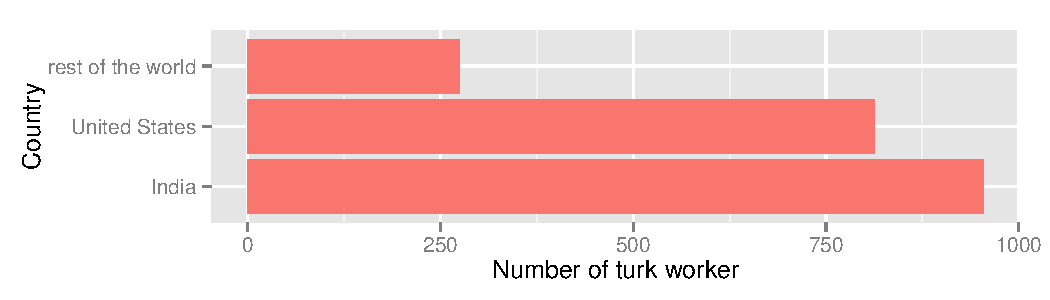
\includegraphics[width=4.5in]{turker_country.pdf} 
   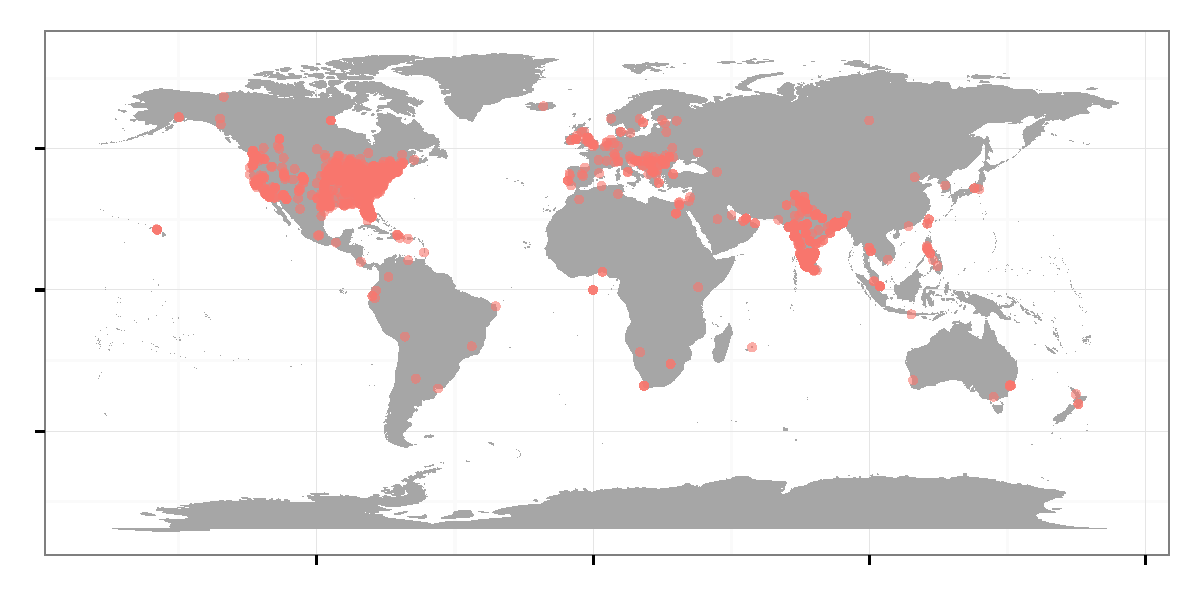
\includegraphics[width=4.5in]{turker_location.pdf}    
   \caption{Location of the Amazon Mechanical Turk workers participating our study. Most of the people are coming from India and United States even though there are people from around the world.}
   \label{fig:turker_location}
\end{figure}

Besides United States and India, countries such as Canada, Romania, United Kingdom and Macedonia have more than 10 participants each. The rest of the 70 countries have less than 10 participants. The distribution of participants remains almost similar in all ten experiments with some small variations (Figure~\ref{fig:turker_location_experiment}). That may be due to the time of the experiment when it first started. For some experiments India got more participants than United States and for some experiments the numbers just got reversed (Figure~\ref{fig:participation_time}). It is also observed in some experiments that number of  participants are similar no matter whether the experiment is run on day time or nigh time.

\begin{table}[hbtp]
\caption{Demographic information of the subjects participated the MTurk experiments. Average time taken for evaluating a lineup is shown in seconds.}
\centering
\scalebox{.85}{
\begin{tabular}{rlrrcr}
  \hline
  && \multicolumn{2}{c}{Participants}&Average&\\
  \cline{3-4}
 Factor & levels & Total &\%Factor & time & response \\ 
  \hline
Gender & Male & 1348&57.63 & 48.51 & 13493 \\ 
   & Female & 991&42.37 & 43.75 & 10564 \\ 
\hline
  Education & High school or less & 193 &8.24& 37.21 & 2241 \\ 
   & Some under graduate courses & 418 & 17.85&42.84 & 4070 \\ 
   & Under graduate degree & 584 &24.93& 44.29 & 5775 \\ 
   & Some graduate courses & 245 &10.46& 43.43 & 2460 \\ 
   & Graduate degree & 902 &38.51& 52.18 & 9511 \\ 
\hline
  Age & 18-25 & 740 &31.61& 42.97 & 7311 \\ 
   & 26-30 & 547 &23.36& 46.27 & 5585 \\ 
   & 31-35 & 376 &16.06& 44.27 & 3923 \\ 
   & 36-40 & 257 &10.98& 55.03 & 2714 \\ 
   & 41-45 & 141 &6.02& 43.90 & 1519 \\ 
   & 46-50 &  95 &4.05& 49.29 & 1003 \\ 
   & 51-55 &  83 &3.54& 48.67 & 867 \\ 
   & 56-60 &  64 & 2.73& 59.73 & 678 \\ 
   & above 60 & 38 &1.62& 48.67 & 457 \\ 
\hline   
  Country  & United States & 1087 &46.83& 39.64 & 10769 \\  
  & India & 980 &42.22& 52.63 & 10227 \\ 
  & Rest of the world & 254&10.94 & 46.86 & 2819 \\ 
  
   \hline
\end{tabular}
}
\label{tbl:demographics}
\end{table}



% This table contains the demographic information without factor wise percentages.
%\begin{table}[hbtp]
%\caption{Demographic information of the subjects participated the MTurk experiments. Average time taken for evaluating a lineup is shown in seconds.}
%\centering
%\scalebox{.9}{
%\begin{tabular}{rlrrr}
%  \hline
% Factor & levels & subjects & avg\_time & response \\ 
%  \hline
%Gender & Male & 1348 & 48.51 & 13493 \\ 
%   & Female & 991 & 43.75 & 10564 \\ 
%\hline
%  Education & High school or less & 193 & 37.21 & 2241 \\ 
%   & Some under graduate courses & 418 & 42.84 & 4070 \\ 
%   & Under graduate degree & 584 & 44.29 & 5775 \\ 
%   & Some graduate courses & 245 & 43.43 & 2460 \\ 
%   & Graduate degree & 902 & 52.18 & 9511 \\ 
%\hline
%  Age & 18-25 & 740 & 42.97 & 7311 \\ 
%   & 26-30 & 547 & 46.27 & 5585 \\ 
%   & 31-35 & 376 & 44.27 & 3923 \\ 
%   & 36-40 & 257 & 55.03 & 2714 \\ 
%   & 41-45 & 141 & 43.90 & 1519 \\ 
%   & 46-50 &  95 & 49.29 & 1003 \\ 
%   & 51-55 &  83 & 48.67 & 867 \\ 
%   & 56-60 &  64 & 59.73 & 678 \\ 
%   & above 60 &  38 & 48.67 & 457 \\ 
%\hline   
%  Country  & United States & 1087 & 39.64 & 10769 \\  
%  & India & 980 & 52.63 & 10227 \\ 
%  & Rest of the world & 254 & 46.86 & 2819 \\ 
%  
%   \hline
%\end{tabular}
%}
%\label{tbl:demographics}
%\end{table}


The largest number of participants are from age group 18 to 25 which is the youngest age group in the study. The majority of the people have ages between 18 to 35. Interestingly there are many participants from older age groups as well. Specially for united states almost all the age groups show uniform participations beyond age 30 (Figure~\ref{fig:demographic_info}). Notice that fewer people participated from India beyond age 40 compared to united states. Total number of participations from india and United States are almost same with United States having 107 more participants. Unlike USA Indian participants are mostly young people. 

In terms of participant's academic background, the largest group is graduate degree. A total of 902 participants have a graduate degree which is about 38.51\%. They are mostly from India as any university degree is considered a graduate degree unlike north America where graduate degree means Masters level education. Most of the USA participants are with an Undergraduate degree or at least have some undergraduate courses (Figure~\ref{fig:demographic_info}). 

The distribution of male and female participants are similar among all age groups except age 18-25 in India where fewer female participants were observed (Figure \ref{fig:gender_country_bar}). The distribution of education levels are also different across the countries for this age group. Most of the participants from India are below age 40 while in United States the distribution of participants are similar beyond age 40. There were not many participants beyond age 50 and hence these age groups are merged to form one age group called above 50. The exploratory analysis and the models fitted in the following sections use this new age group instead of actual age groups beyond age 50. 

A total of 1911 lineups were evaluated in the ten experiments. Each person evaluated at least 10 lineups except for experiment 9 where three lineups were evaluated by each person. A test plot was shown to each observer and the feedback received from that plot is used to examine the data quality or process payment. But the data received for the test lineup is not included in the analysis. In some cases the demographic information were not provided by the participants. Also, for some ip address, the actual geographical locations could not be retrieved. This resulted some missing demographic information.

\subsection{Demographic Factors} Proportions of correct responses and natural logarithms of average time taken to evaluate  each lineup are computed  for different demographic factor levels. Their distributions are shown using boxplots in Figure \ref{fig:demographic_effect}. Averages of these distributions are represented by dots inside the boxplots. The youngest age group (18-25) took least average time to evaluate a lineup. People from India took more time than others. People who have only a high school degree took less time and this is related to what we have seen for young age group. Averages of log time taken by male and female participants look similar but there are some differences as we see in Table~\ref{tbl:demographics}. 

%All of the factors are significant in describing time taken to evaluate a lineup.

\begin{figure}[htbp] 
   \centering
   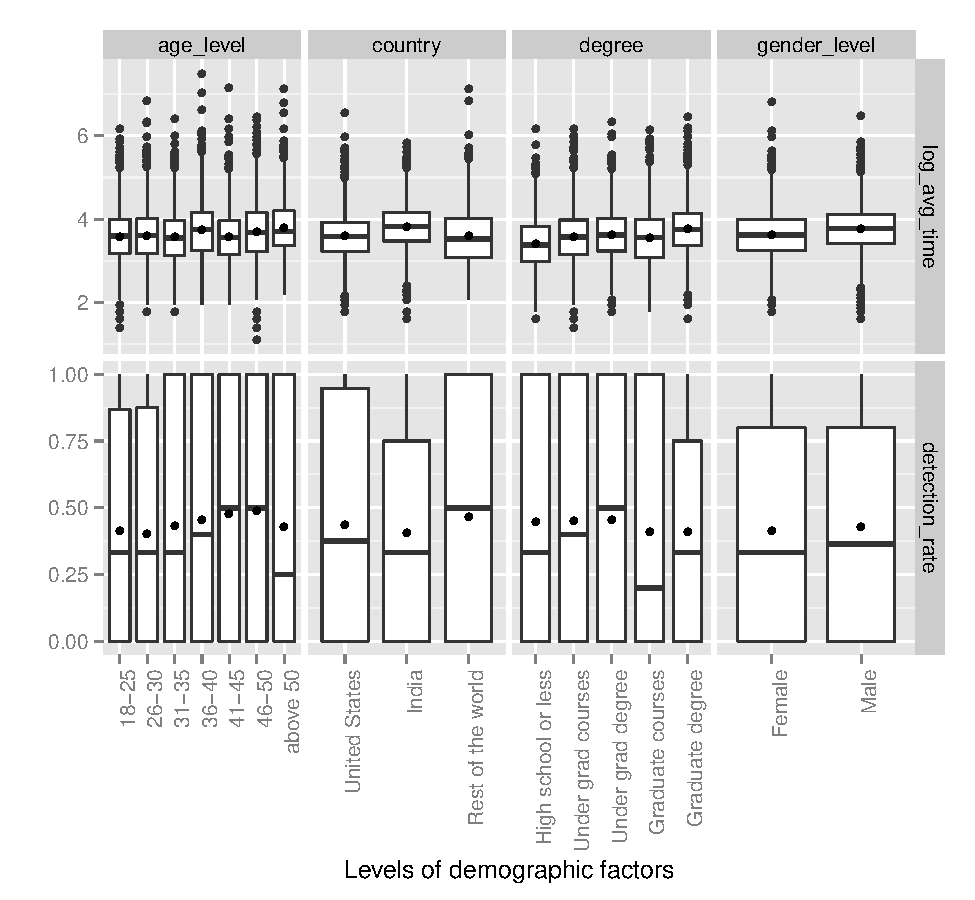
\includegraphics[width=4in]{demographic_effect.pdf} 
   \caption{Boxplots of average log time taken and proportion correct responses of all the lineups plotted for each demographic factor levels. The dots inside the boxes represent means. Some differences in means of various demographic factors are observed. Variability in proportion correct indicates large variability in lineup difficulties.}
   \label{fig:demographic_effect}
\end{figure}

The distribution of time taken to evaluate a lineup is positively skewed. But in log scale it appears to be symmetric for all the demographic factor variables as we see in Figure \ref{fig:demographic_effect}. Mean and medians are very similar as well. This allows us to fit linear mixed model to the log time taken with normal error structure.

We observed some differences in median proportion of correct responses for different demographic factor levels. But the variability of proportion correct responses are huge as per design of the experiments since there were some very easy as well as extremely difficult lineups. Some of the lineups  were not expected to be evaluated correctly as the null plots in those lineups were showing more signal than the actual data plot itself. In those scenarios,  one may not reject the null hypothesis. We call these difficult lineups. Some of the lineups were so easy that data plot is detectable at a first glance. These were expected to be evaluated correctly 100\% of the time. This is why we see the boxes range from 0 to 1 in most of the factor levels. Unlike median, fewer differences are observed in the average proportion of correct responses for different factor levels. 

Model \eqref{eqn:demographic_response} is fitted to the data with fixed effect factors such as age, country, education and gender. To estimate the overall factor main effect, a reduced model is fitted removing that factor from Model \eqref{eqn:demographic_response}. Analysis of variance (ANOVA)  results shown in Table~\ref{tbl:anova_factor} suggest that all the factor variables are significantly different in describing the the probability of correct response except gender. Gender does not show any significant difference in performance.  Similarly, ANOVA results are obtained by fitting Model \eqref{eqn:demographic_time} to the data of log time taken and are shown in Table~\ref{tbl:anova_factor} as well. All the factor variables are significantly different for log time taken including gender.  

\begin{table}[htbp]
\centering
\caption{Anova of full model with all the demographic factors vs reduced model with removing respective factor variable. Gender does not have any effect on probability of correct response.}
\scalebox{.9}{
\begin{tabular}{rlrrrrrr}
  \hline
Model & & AIC & BIC & logLik & Chisq & Chi.Df & $p$-value \\ 
  \hline
Proportion Correct &Full & 23822.00 &23943.00 &-11896.00  & &  &  \\ 
& \multicolumn{2}{l}{Reduced}  &  &  &  & \\
  &Age & 23835.22 & 23907.93 & -11908.61 & 25.50 & 6 & $<$0.001 \\ 
  &Country  & 24099.57 & 24204.72 & -12036.78 & 281.85 & 2 & $<$0.001 \\ 
  &Education  & 23837.48 & 23926.34 & -11907.74 & 23.77 & 4 & $<$0.001 \\ 
  &Gender  & 23821.88 & 23934.98 & -11896.94 & 2.17 & 1 & 0.140 \\ 
   \hline
   Log Time &Full &  51904.00 &52034.00 & -25936.00 & &  &  \\ 
& \multicolumn{2}{l}{Reduced}  &  &  &  & \\
&Age  & 52435.63 & 52516.41 & -26207.81 & 543.18 & 6 & $<$0.001 \\ 
 & Country  & 52849.92 & 52963.15 & -26410.96 & 949.47 & 2 & $<$0.001 \\ 
  &Education  & 52012.68 & 52109.61 & -25994.34 & 116.23 & 4 & $<$0.001 \\ 
  &Gender  & 51970.57 & 52091.74 & -25970.28 & 68.12 & 1 & $<$0.001 \\ 
\hline
\end{tabular}
}
\label{tbl:anova_factor}
\end{table}


To further illustrate how the individual factor levels differ from each other  the detailed results of Models \eqref{eqn:demographic_response} and \eqref{eqn:demographic_time} are shown in Table \ref{tbl:model_result_demographics}. For parameter estimation the first factor levels shown in the Table are  used as the base line. Demographic factor levels have significant effects on log time taken to evaluate a lineup. But not all the levels are significant for the probability of correct responses.


\begin{table}[htbp]
\centering
\caption{Parameter estimates of Models \eqref{eqn:demographic_time} and \eqref{eqn:demographic_response} fitted for average log time taken and probability of correct lineup evaluations respectively. For time taken all the demographic factors are significant. For probability of correct response age group 36-40, rest of the world and graduate degree are significantly different. For gender no difference in performance is observed. Lineup variability is estimated to be very large for Model \eqref{eqn:demographic_response}.}
\scalebox{0.86}{
\begin{tabular}{rlrrrrrrrrrr}
  \hline
Demographic&& \multicolumn{4}{c} {Model \eqref{eqn:demographic_time} Log Time} & &\multicolumn{4}{c} {Model \eqref{eqn:demographic_response} Proportion Correct} \\

\cline{3-6} \cline{8-11} 
Factor & Level& Est & SE & Zval & $p$-value && Est & SE & Zval & $p$-value  \\ 
  \hline
\multicolumn{2}{l}{Fixed Effect} &  &  &  &  &  & & && \\ 
&$\mu$ & 3.360 & 0.013 & 249.21 & $<$0.001 &   & -0.683 & 0.071 & -9.64 & $<$0.001 \\ 
\hline
Age ($\alpha$)& 18-25&0.000   &---  &---  &---  &  &--- &--- &---& ---\\   
 &26-30 & 0.058 & 0.013 & 4.50 & $<$0.001 &   & 0.062 & 0.049 & 1.27 & 0.206 \\ 
  &31-35 & 0.068 & 0.014 & 4.72 & $<$0.001 &   & 0.115 & 0.055 & 2.08 & 0.038 \\ 
  &36-40 & 0.231 & 0.016 & 14.05 & $<$0.001 &   & 0.310 & 0.063 & 4.93 & $<$0.001 \\ 
  &41-45 & 0.176 & 0.021 & 8.56 & $<$0.001 &   & 0.158 & 0.081 & 1.96 & 0.050 \\ 
  &46-50 & 0.272 & 0.024 & 11.29 & $<$0.001 &   & 0.141 & 0.096 & 1.47 & 0.143 \\ 
  &above 50 & 0.352 & 0.018 & 19.19 & $<$0.001 &   & 0.147 & 0.071 & 2.06 & 0.039 \\ 
  \hline
Country($\kappa$)& United States&0.000   &---  &---  &---  &  &--- &--- &---& ---\\  
  &India & 0.101 & 0.011 & 9.11 & $<$0.001 &   & 0.058 & 0.043 & 1.33 & 0.183 \\ 
  &Rest of world & -0.129 & 0.009 & -13.82 & $<$0.001 &   & 0.185 & 0.035 & 5.22 & $<$0.001 \\ 
  \hline
Education($\tau$) &High school or less&0.000   &---  &---  &---  &  &--- &--- &---& ---\\     
 &Under grad courses & 0.042 & 0.013 & 3.25 & 0.0011 &   & -0.083 & 0.050 & -1.65 & 0.098 \\ 
  &Under grad degree & -0.037 & 0.012 & -3.21 & 0.0013 &   & -0.044 & 0.045 & -0.97 & 0.331 \\ 
  &Graduate courses & 0.117 & 0.013 & 9.12 & $<$0.001 &   & 0.070 & 0.050 & 1.42 & 0.157 \\ 
  &Graduate degree & 0.046 & 0.011 & 4.12 & $<$0.001 &   & 0.182 & 0.043 & 4.22 & $<$0.001 \\ 
  \hline
Gender ($\gamma$)& Female&0.000   &---  &---  &---  &  &--- &--- &---& ---\\      
  &Male & 0.078 & 0.009 & 8.26 & $<$0.001 &   & 0.055 & 0.036 & 1.50 & 0.133 \\ 
  \hline
\multicolumn{2}{l}{Random Effect} &  &  &  &  &  & & && \\ 
& lineup($\sigma_{\ell}$) & 0.082 & 0.287 &  &  &   & 5.259 & 2.293 &  &  \\ 
 & Error($\sigma$) & 0.479 & 0.692 &  &  & & && &\\ 
   \hline
\end{tabular}
}
\label{tbl:model_result_demographics}
\end{table}



% This table had 4 digits $p$-value for last column
%\begin{table}[htbp]
%\centering
%\caption{Parameter estimates of Models \eqref{eqn:demographic_time} and \eqref{eqn:demographic_response} fitted for average log time taken and probability of correct lineup evaluations respectively. For time taken all the demographic factors are significant. For probability of correct response age group 36-40, rest of the world and graduate degree are significantly different. For gender no difference in performance is observed. Lineup variability is estimated to be very large for Model \eqref{eqn:demographic_response}.}
%\scalebox{0.86}{
%\begin{tabular}{rlrrrrrrrrrr}
%  \hline
%Demographic&& \multicolumn{4}{c} {Model \eqref{eqn:demographic_time} Log Time} & &\multicolumn{4}{c} {Model \eqref{eqn:demographic_response} Proportion Correct} \\
%
%\cline{3-6} \cline{8-11} 
%Factor & Level& Est & SE & Zval & $p$-value && Est & SE & Zval & $p$-value  \\ 
%  \hline
%\multicolumn{2}{l}{Fixed Effect} &  &  &  &  &  & & && \\ 
%&$\mu$ & 3.360 & 0.013 & 249.21 & $<$0.001 &   & -0.683 & 0.071 & -9.64 & $<$0.001 \\ 
%\hline
%Age ($\alpha$)& 18-25&0.000   &---  &---  &---  &  &--- &--- &---& ---\\   
% &26-30 & 0.058 & 0.013 & 4.50 & $<$0.001 &   & 0.062 & 0.049 & 1.27 & 0.2058 \\ 
%  &31-35 & 0.068 & 0.014 & 4.72 & $<$0.001 &   & 0.115 & 0.055 & 2.08 & 0.0376 \\ 
%  &36-40 & 0.231 & 0.016 & 14.05 & $<$0.001 &   & 0.310 & 0.063 & 4.93 & $<$0.001 \\ 
%  &41-45 & 0.176 & 0.021 & 8.56 & $<$0.001 &   & 0.158 & 0.081 & 1.96 & 0.0501 \\ 
%  &46-50 & 0.272 & 0.024 & 11.29 & $<$0.001 &   & 0.141 & 0.096 & 1.47 & 0.1425 \\ 
%  &above 50 & 0.352 & 0.018 & 19.19 & $<$0.001 &   & 0.147 & 0.071 & 2.06 & 0.0394 \\ 
%  \hline
%Country($\kappa$)& United States&0.000   &---  &---  &---  &  &--- &--- &---& ---\\  
%  &India & 0.101 & 0.011 & 9.11 & $<$0.001 &   & 0.058 & 0.043 & 1.33 & 0.183 \\ 
%  &Rest of world & -0.129 & 0.009 & -13.82 & $<$0.001 &   & 0.185 & 0.035 & 5.22 & $<$0.001 \\ 
%  \hline
%Education($\tau$) &High school or less&0.000   &---  &---  &---  &  &--- &--- &---& ---\\     
% &Under grad courses & 0.042 & 0.013 & 3.25 & 0.0011 &   & -0.083 & 0.050 & -1.65 & 0.098 \\ 
%  &Under grad degree & -0.037 & 0.012 & -3.21 & 0.0013 &   & -0.044 & 0.045 & -0.97 & 0.3307 \\ 
%  &Graduate courses & 0.117 & 0.013 & 9.12 & $<$0.001 &   & 0.070 & 0.050 & 1.42 & 0.1566 \\ 
%  &Graduate degree & 0.046 & 0.011 & 4.12 & $<$0.001 &   & 0.182 & 0.043 & 4.22 & $<$0.001 \\ 
%  \hline
%Gender ($\gamma$)& Female&0.000   &---  &---  &---  &  &--- &--- &---& ---\\      
%  &Male & 0.078 & 0.009 & 8.26 & $<$0.001 &   & 0.055 & 0.036 & 1.50 & 0.1331 \\ 
%  \hline
%\multicolumn{2}{l}{Random Effect} &  &  &  &  &  & & && \\ 
%& lineup($\sigma_{\ell}$) & 0.082 & 0.287 &  &  &   & 5.259 & 2.293 &  &  \\ 
% & Error($\sigma$) & 0.479 & 0.692 &  &  & & && &\\ 
%   \hline
%\end{tabular}
%}
%\label{tbl:model_result_demographics}
%\end{table}

Age group 36-40 is significantly different than the base line age group of 18-25 year olds. The other age levels are similar in explaining the probability of correct response. For country, the rest of the world is different from USA but India appears to be similar to USA. We see from Table \ref{tbl:demographics} that most of the participants (about 90\%) are from India and USA. The rest of the 10\% data are from 76 different countries. This diversity in the rest of the world may make it different from India and USA.

The graduate degree holders are significantly different as well. The positive parameter estimate indicates that they perform better and the probability of correct response is higher than other education levels. There is no significant difference between male and female performances. 

Notice that lineup specific variance estimate is 5.259 with a standard error of 2.293 which is much higher than the other significant parameter estimates in Model \eqref{eqn:demographic_response}. This indicates that the major and most important factor affecting the probability of correct response is  lineup difficulty. This is also evident from the large variability in the proportion correct in Figure~\ref{fig:demographic_effect}. Because of this huge impact of lineup specific variance, the practical impact of other factor variables on the probability of correct response is in fact very small. We illustrate this with the following example of graduate degree.

While some of the demographic factors are strongly statistically significant, the main source of variation in proportion correct is the lineup difficulty. For example, let's examine the effect of graduate degree. To see just how large the effect is, we examine the change in proportion correct for a (hypothetical) 18-25 year old female in the United States, with a graduate degree as compared to a high school degree, for an average difficulty lineup (random effect = 0). Plugging in the relevant quantities to the fitted model gives a difference equal to:
$$ \frac {\exp(-0.683+0.182)}{1+\exp(-0.683+0.182)}-  \frac {\exp(-0.683)}{1+\exp(-0.683)} = 0.377- 0.336 =0.041.$$ 
The person with a high school education on average picks the data plot in 33.5\% of lineups having average difficulty, as compare to 37.6\% if they have a graduate degree. This difference is reduced to 2\% for a lineup with one standard deviation order of magnitude difference in difficulty. For two standard deviations it further reduces to 0.3\%. Thus although there is statstically significant difference in proportion correct for some demographic factors, these are not practically significant differences.  Figure~\ref{fig:practical_impact_graduate} illustrates this example showing fitted models for a US 18-25 female with either a high school education or a graduate degree.  Similar calculations show the same negligible impact of age level 36-40 (0.0533 at most)  and country (0.0424 at most) on the probability of correct response. Thus even though some of the demographic factors are statistically significant, practically, demographics do not substantially influence the results. 

\begin{figure}[htbp] 
   \centering
%   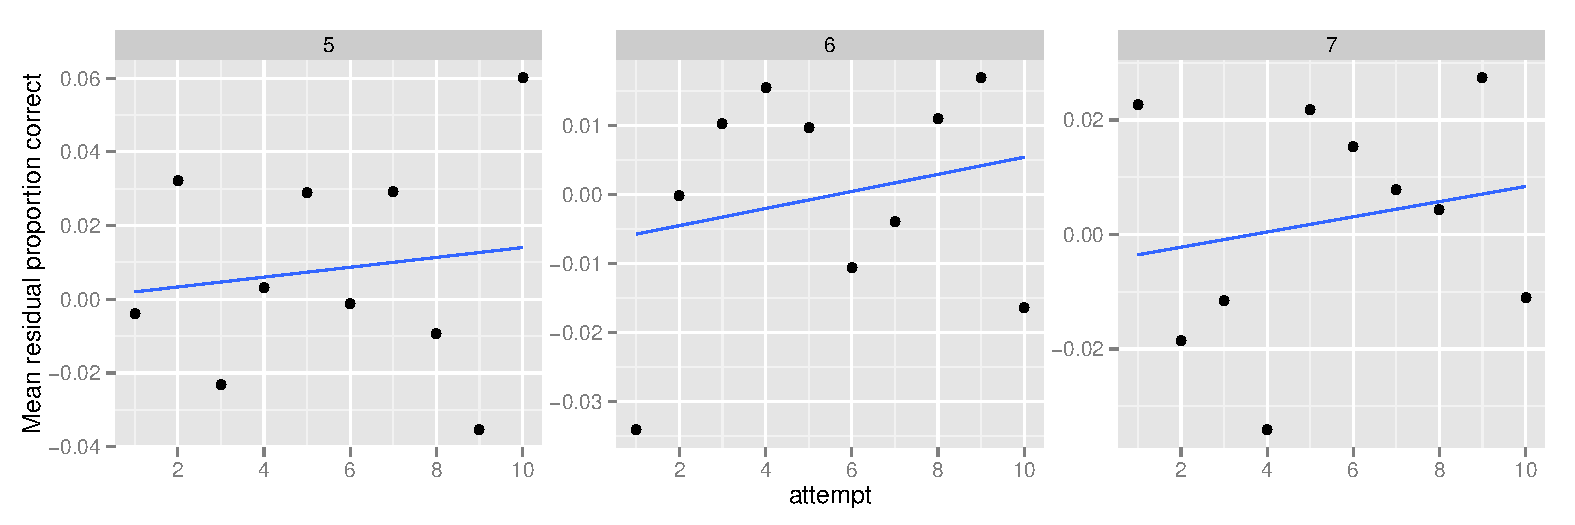
\includegraphics[width=6.5in]{learning_trend.pdf} 
    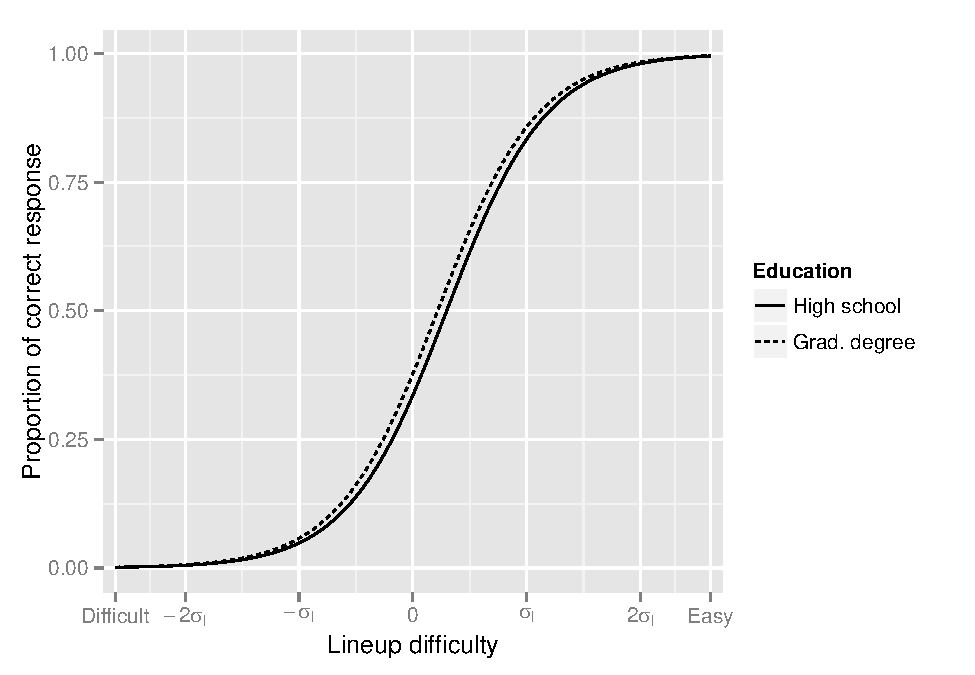
\includegraphics[width=3.0in]{practical_impact_graduate.pdf} 
    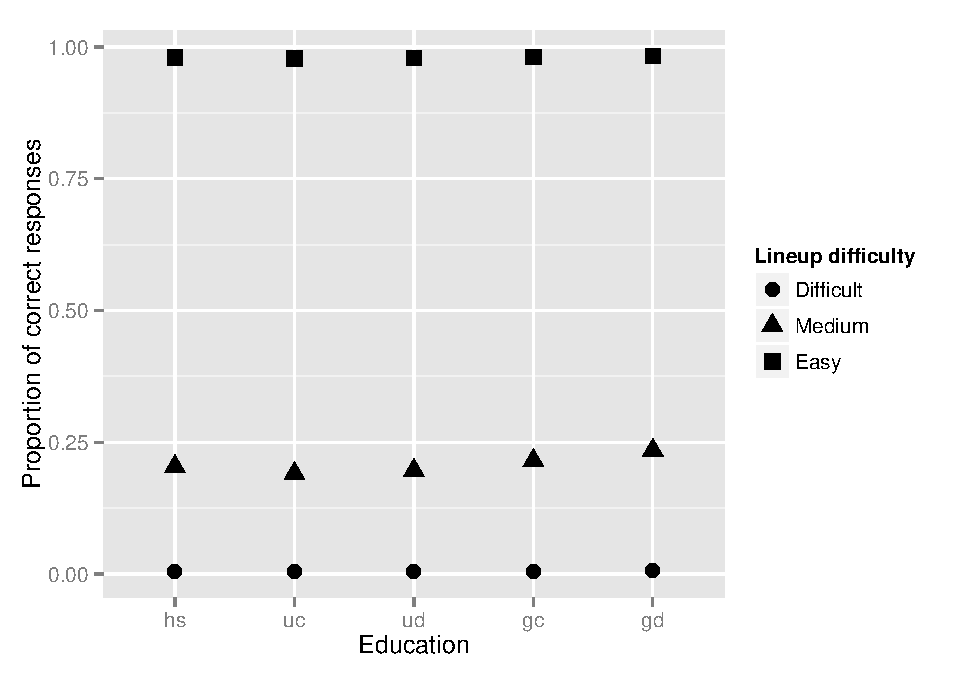
\includegraphics[width=3.0in]{practical_impact_degree.pdf} 
   \caption{Proportion of correct responses due to graduate degree as compared to high school degree for an 18-25 year old female in the United States. Even though graduate degree is statistically significant, the largest difference in proportion correct is  0.045 which is very negligible. The difference diminishes as we move away one or two standard deviations ($\sigma_{\ell} =2.293$) of lineup variability.}
   \label{fig:practical_impact_graduate}
\end{figure}


%\begin{figure}[htbp] 
%   \centering
%%   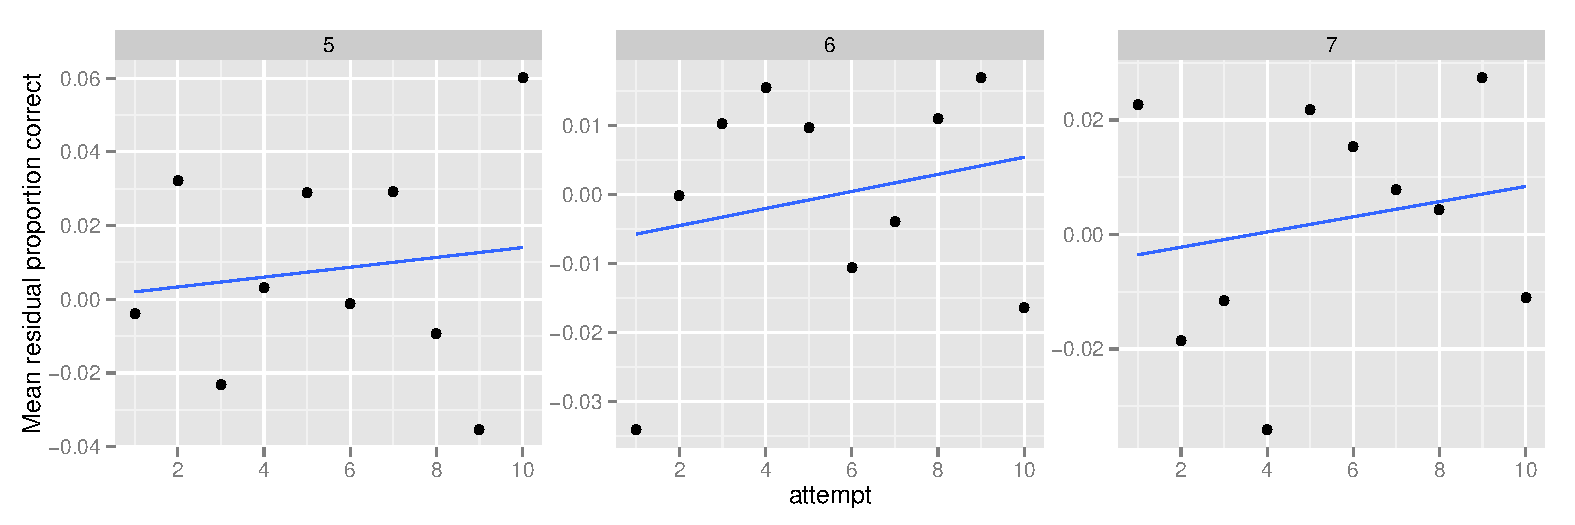
\includegraphics[width=6.5in]{learning_trend.pdf} 
%    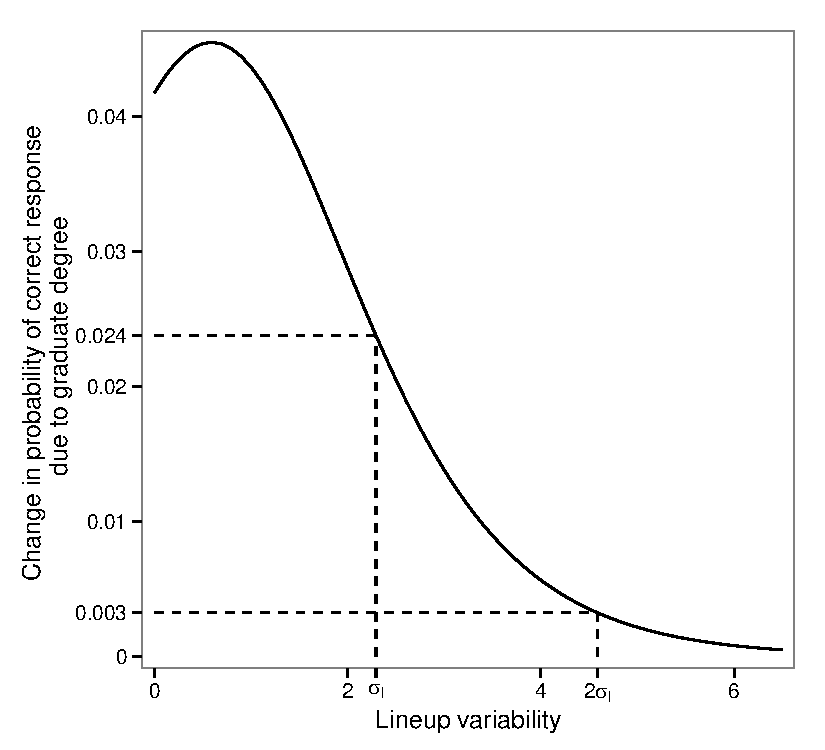
\includegraphics[width=3in]{practical_impact_demographics.pdf} 
%   \caption{ Change in probability of correct response due to graduate degree as compared to high school degree diminishes rapidly as the variability in lineup difficulty $\sigma_{\ell}$ increases.}
%   \label{fig:practical_impact_demographics}
%\end{figure}




%Model \eqref{eqn:demographic_time} is fitted for the log time taken to evaluate a lineup and the results are also shown in  Table~\ref{tbl:model_result_demographics}.  The effect of all the demographic factors on log time taken to evaluate a lineup appears to be significant. 



%
%\begin{table}[htbp]
%\centering
%\caption{Anova of full model with all the demographic factors vs reduced model with removing respective factor.}
%\begin{tabular}{lrrrrrrrr}
%  \hline
%Model && Df & AIC & BIC & logLik & Chisq & Chi.Df & $p$-value \\ 
%  \hline
%Log Time &Full& 16 &  51904.00 &52034.00 & -25936.00 & &  &  \\ 
%& \multicolumn{2}{l}{Reduced} &  &  &  &  & \\
%&Age & 10 & 52435.63 & 52516.41 & -26207.81 & 543.18 & 6 & $<$0.001 \\ 
% & Country & 14 & 52849.92 & 52963.15 & -26410.96 & 949.47 & 2 & $<$0.001 \\ 
%  &Education & 12 & 52012.68 & 52109.61 & -25994.34 & 116.23 & 4 & $<$0.001 \\ 
%  &Gender & 15 & 51970.57 & 52091.74 & -25970.28 & 68.12 & 1 & $<$0.001 \\ 
%\hline
%Proportion Correct &Full& 15 & 23822.00 &23943.00 &-11896.00  & &  &  \\ 
%& \multicolumn{2}{l}{Reduced} &  &  &  &  & \\
%  &Age & 9 & 23835.22 & 23907.93 & -11908.61 & 25.50 & 6 & $<$0.001 \\ 
%  &Country & 13 & 24099.57 & 24204.72 & -12036.78 & 281.85 & 2 & $<$0.001 \\ 
%  &Education & 11 & 23837.48 & 23926.34 & -11907.74 & 23.77 & 4 & $<$0.001 \\ 
%  &Gender & 14 & 23821.88 & 23934.98 & -11896.94 & 2.17 & 1 & 0.140 \\ 
%   \hline
%\end{tabular}
%\end{table}
%


\subsection{Learning Trend} Models \eqref{eqn:trend_response} and \eqref{eqn:trend_time} are fitted to the data from experiment 5, 6, and 7 separately.  As an alternative to Model \eqref{eqn:trend_response} we examined a reduced model with attempt as a continuous covariate. They did not appear to be significantly different with a $p$-value of 0.856. But we consider the bigger Model \eqref{eqn:trend_response} with attempt as a factor variable with 10 levels to examine the effect of each level. Attempt 1 is considered to be base level while fitting the model.

Table \ref{tbl:model_result_response} presents the parameter estimates and $p$-values of fixed effect estimates of Model \eqref{eqn:trend_response}. The larger $p$-values suggest that none of the levels of attempt ($\alpha_2$ through $\alpha_{10}$) are significant at \%1 significance level. Moreover, some of the estimates are positive and some are negative and they show up seemingly in random order suggesting later attempts not necessarily have improved. This indicates that there may be no learning effect on the probability of correct evaluations. 


\begin{table}[htbp]
\centering
\caption{Parameter estimates of Model \eqref{eqn:trend_response} fitted for probability of correct lineup evaluation. None of the fixed factor effects of attempt ($\alpha_2$ through $\alpha_{10}$) are significantly different from the first attempt $\alpha_1$
at \%1 level in all three experiments 5, 6 and 7. For experiment 7 subject specific variation is very small on the other hand lineup variance is much higher compared to the other two experiments.}
\scalebox{0.81}{
\begin{tabular}{rrrrccrrrccrrrc}
  \hline
& \multicolumn{4}{c} {Experiment 5} & &\multicolumn{4}{c} {Experiment 6} && \multicolumn{4}{c} {Experiment 7}\\

\cline{2-5} \cline{7-10} \cline{12-15} 
 Effect& Est & SE & Zval & $p$-value && Est & SE & Zval & $p$-value && Est & SE & Zval & $p$-value \\ 
  \hline
Fixed &  &  &  & && &  & & & & & &  & \\ 
$\mu$ & -1.304 & 0.179 & -7.28 & $<$0.001 &   & -0.220 & 0.147 & -1.50 & 0.134 &   & -1.737 & 0.481 & -3.61 & $<$0.001 \\ 
  $\alpha_1$ & 0.000 & --- & --- & --- &   & 0.000 & --- & --- & --- &  & 0.000 & --- & --- & ---  \\ 
  $\alpha_2$ & 0.270 & 0.219 & 1.24 & 0.217 &   & 0.262 & 0.158 & 1.66 & 0.098 &   & -0.456 & 0.385 & -1.18 & 0.237 \\ 
  $\alpha_3$ & -0.178 & 0.226 & -0.79 & 0.432 &   & 0.342 & 0.157 & 2.18 & 0.029 &   & -0.105 & 0.386 & -0.27 & 0.786 \\ 
  $\alpha_4$ & 0.083 & 0.224 & 0.37 & 0.712 &   & 0.358 & 0.159 & 2.26 & 0.024 &   & -0.378 & 0.381 & -0.99 & 0.322 \\ 
  $\alpha_5$ & 0.298 & 0.224 & 1.33 & 0.183 &   & 0.376 & 0.159 & 2.36 & 0.018 &   & -0.107 & 0.385 & -0.28 & 0.781 \\ 
  $\alpha_6$ & 0.042 & 0.231 & 0.18 & 0.857 &   & 0.246 & 0.158 & 1.56 & 0.120 &   & 0.026 & 0.407 & 0.06 & 0.949 \\ 
  $\alpha_7$ & 0.283 & 0.230 & 1.23 & 0.217 &   & 0.160 & 0.159 & 1.01 & 0.314 &   & 0.057 & 0.401 & 0.14 & 0.886 \\ 
  $\alpha_8$ & -0.045 & 0.233 & -0.19 & 0.847 &   & 0.341 & 0.160 & 2.13 & 0.033 &   & -0.003 & 0.394 & -0.01 & 0.994 \\ 
  $\alpha_9$ & -0.195 & 0.232 & -0.84 & 0.400 &   & 0.378 & 0.160 & 2.36 & 0.018 &   & 0.204 & 0.436 & 0.47 & 0.639 \\ 
  $\alpha_{10}$ & 0.513 & 0.228 & 2.25 & 0.024 &   & 0.192 & 0.163 & 1.18 & 0.238 &   & -0.213 & 0.432 & -0.49 & 0.622 \\ 
\multicolumn{2}{l}{Random}   &  &  &  &  & & &&& & & &  & \\ 
  $\sigma^2_a$ & $<$0.001 & 0.017 &  &  &   & 0.001 & 0.034 &  &  &   & 0.027 & 0.163 &  &  \\ 
  $\sigma^2_u$ & 0.720 & 0.848 &  &  &   & 0.815 & 0.903 &  &  &   & $<$0.001 & $<$0.001 &  &  \\ 
  $\sigma^2_{\ell}$ & 2.178 & 1.476 &  &  &   & 2.009 & 1.418 &  &  &   & 10.980 & 3.314 &  &  \\ 
   \hline
\end{tabular}
}
\label{tbl:model_result_response}
\end{table}


The variance of random slope for attempt ($\sigma^2_a$) is estimated to be very small compared to other random effects except for subject variability ($\sigma^2_u$) for experiment 7. This suggests that most of the variability for attempt is accounted for by the fixed effect factor attempt. For all three experiments the lineup variabilities ($\sigma^2_l$) were estimated to be very large making the practical impact of other factor levels even more negligible. Some of the lineups were very easy and some were really difficult in experiment 7. The overall average probability for picking out the data plot from a lineup ($\mu$) is significant for both experiments 5 and 7. But for experiment 6 it is not significant suggesting that experiment 6 lineups were difficult compared to the other experimental lineups. This shows a feature of the experimental designs where a mixture of difficult and easy lineups were included within the experiments as well as between the experiments.  For easy lineups there may be small chance to improve performances. But for harder lineups, the scope to improve performances is large.  Since for none of these experiments improvement in performances is observed, it is important in the sense that performances did not improve over attempts in both difficult and easy lineup situations.

%The results are shown in Tables \ref{tbl:model_result_response} \ref{tbl:model_result_time}.


%Model \eqref{eqn:trend_time} is fitted to the data from experiment 5, 6, and 7 separately.   For this the function $lmer()$ is used from R package $lme4$ by \cite{lme4:2011}. To obtain the $p$-values of fixed effect parameters estimates, normal approximation is used for $Z$ scores computed as the ratio of estimates to the estimated standard errors. The results are shown in Table \ref{tbl:model_result_time}. Both fixed effect parameters of covariate Attempt ($\alpha_1$ and $\alpha$) are highly significant.

%Each subject participating the experiment has seen multiple number of lineups for evaluations. Suppose $K$ be the number of lineups evaluated by a subject and $A_k$ be the $kth$ attempt, $k=1,2, ..., K$. Subjects may have a chance for self learning and do better on lineups shown later in the sequence. They may learn from their previous mistake or they may learn about the features of the plots being evaluated as they progress. Thus if there is any learning trend that should be apparent in proportion correct over $A_k$. But to obtain this we have to adjust for lineup difficulty and individual performances.

To visualize how the performance in correct response improves over successive attempts, we fitted Model \eqref{eqn:trend_response} excluding the covariates related to attempt from the model and computed the residuals. Least square regression lines were fitted through the subject specific residuals as shown in Figure~\ref{fig:learning_trend_response}. Two important features were observed; one is subject specific variability and the other is random slope with attempts which indicates subjects specific learning trend. Some subjects show improvement over time and some show the decrease in performance. 

\begin{figure}[htbp] 
   \centering
%   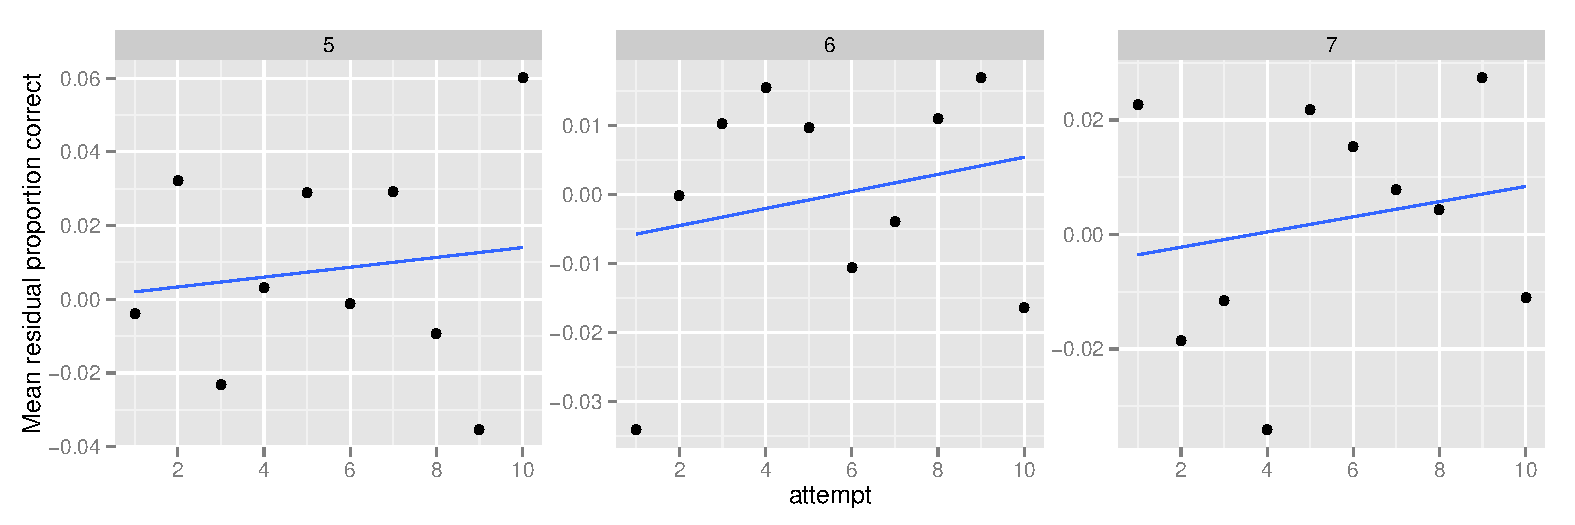
\includegraphics[width=6.5in]{learning_trend.pdf} 
    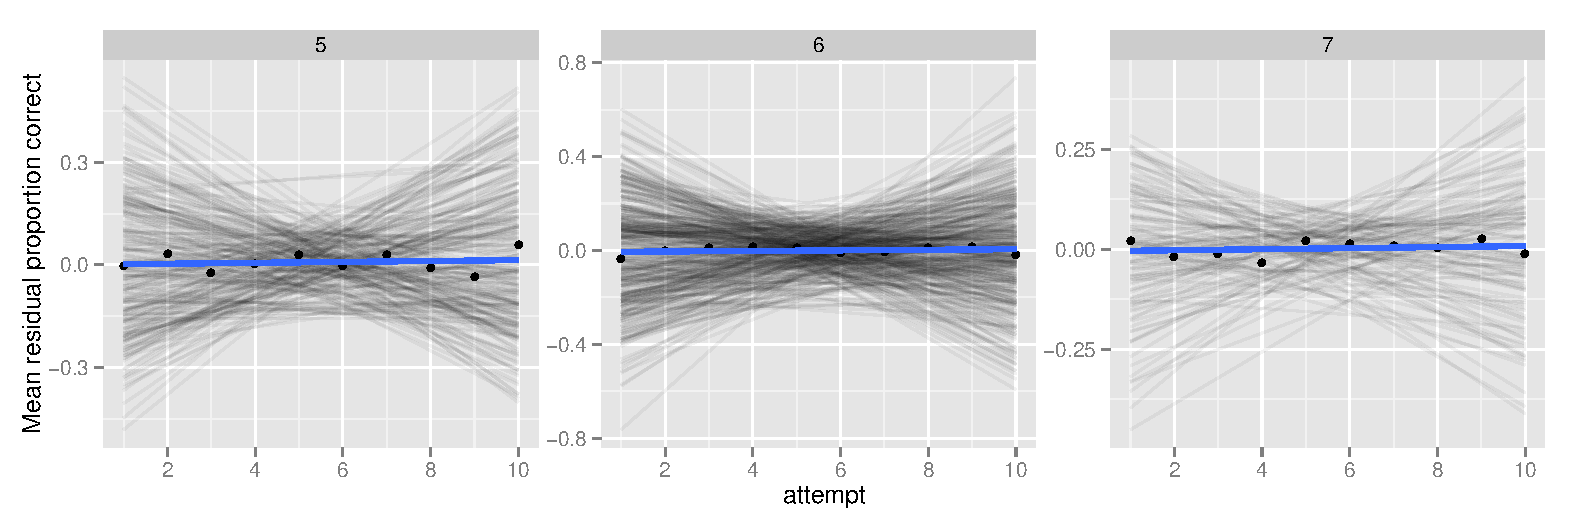
\includegraphics[width=6.3in]{learning_trend_subject.pdf} 
   \caption{ Least square lines fitted through the subject specific residual proportion correct obtained from Model \eqref{eqn:trend_response} fitted without attempt are plotted against attempt. Subject specific positive and negative slopes are observed. Mean residuals are shown as dots and least square regression lines fitted through the points show no overall learning trend in each of the three experiments.}
   \label{fig:learning_trend_response}
\end{figure}

The averages of these residuals for each of the attempts are shown as dots in Figure~\ref{fig:learning_trend_response}. Least square linear regression lines are fitted through the points for each of the experiments. Positive slopes over the attempts are observed but none of them is statistically significant. 

Table \ref{tbl:model_result_time} presents the results of Model \eqref{eqn:trend_time}. The parameter $\alpha$ for fixed effect covariate attempt is highly significant in all the experiments. The negative estimates suggest that on an average later attempt took less time for an evaluation. Even though observers did not improve the performance over attempt, they became efficient in responding faster. The parameter $\alpha_1$ for first attempt is also highly significant. The positive estimates of $\alpha_1$ indicates that first attempt made by an observer required much more times than other attempts. It is because for initial attempt the observer might have gone through instructions and became familiar with the experimental environment. Each page in the web site contains information about choice reason and the observers's confidence level. Also, the first page asks for observer Identification to be typed. The later pages of the web site was similar just the lineup was changed. Thus in the later attempts an observer does not need to spend any time for reading instructions. The model reflects that fact.


\begin{table}[htbp]
\centering
\caption{Parameter estimates of Model \eqref{eqn:trend_time} fitted for log time taken to evaluate a lineup. Both fixed effect parameters of Attempt ($\alpha_1$ and $\alpha$) are highly significant for all three experiments 5, 6 and 7.}
\scalebox{0.81}{
\begin{tabular}{rrrrccrrrccrrrc}
  \hline
& \multicolumn{4}{c} {Experiment 5} & &\multicolumn{4}{c} {Experiment 6} && \multicolumn{4}{c} {Experiment 7}\\

\cline{2-5} \cline{7-10} \cline{12-15} 
 Effect& Est & SE & Zval & $p$-value && Est & SE & Zval & $p$-value && Est & SE & Zval & $p$-value \\ 
  \hline
Fixed &  &  &  & && &  & & & & & &  & \\ 
$\mu$ & 3.817 & 0.039 & 97.38 & $<$0.001 &   & 3.901 & 0.033 & 118.19 & $<$0.001 &   & 3.731 & 0.054 & 69.04 & $<$0.001 \\ 
  $\alpha_1$ & 0.326 & 0.035 & 9.35 & $<$0.001 &   & 0.335 & 0.029 & 11.40 & $<$0.001 &   & 0.280 & 0.050 & 5.63 & $<$0.001 \\ 
  $\alpha$ & -0.038 & 0.004 & -9.30 & $<$0.001 &   & -0.039 & 0.004 & -10.19 & $<$0.001 &   & -0.029 & 0.007 & -4.22 & $<$0.001 \\ 
\multicolumn{2}{l}{Random}   &  &  &  &  & & &&& & & &  & \\ 
  $\sigma^2_a$ & 0.001 & 0.027 &  &  &   & 0.002 & 0.045 &  &  &   & 0.002 & 0.049 &  &  \\ 
  $\sigma^2_u$ & 0.259 & 0.509 &  &  &   & 0.245 & 0.495 &  &  &   & 0.134 & 0.366 &  &  \\ 
  $\sigma^2_{\ell}$ & 0.008 & 0.091 &  &  &   & 0.040 & 0.199 &  &  &   & 0.055 & 0.235 &  &  \\ 
  $\sigma^2$ & 0.211 & 0.460 &  &  &   & 0.251 & 0.501 &  &  &   & 0.206 & 0.454 &  &  \\ 
   \hline
\end{tabular}
}
\label{tbl:model_result_time}
\end{table}

The lineup variance of experiment 7 is estimated as $\hat{\sigma}^2_{\ell} = 10.98$ from Model \eqref{eqn:trend_response}. But from Model \eqref{eqn:trend_time} it is estimated to be much smaller in all these experiments. This suggests that the harder lineups not necessarily took more time than easier lineups. The observers spent enough times to evaluate a easy lineup and for difficult lineup they might just give up at some point and provided the feedback.

Model \eqref{eqn:trend_time} was compared to couple of other alternatives. A bigger model with attempt as a factor was considered but it was not significantly different with $p$ value 0.236. A reduced model without the first attempt was also considered but it was significantly different with $p$-value $<0.001$. 

To visualize how the time taken reduces over the successive attempts, we fitted Model \eqref{eqn:trend_time} excluding the covariate attempt from the model and computed the residuals. Least square regression lines are fitted through the subject specific residuals. Subject specific slopes are much different in each of the three experiments as we see in Figure \ref{fig:learning_trend_time}. Some subjects improved over attempts by taking less time in the later attempts while others got worse. The averages of these residuals for each attempt are plotted as dots. Least square regression lines are fitted to these points excluding the first attempt since for first attempt we fitted an indicator covariate. The downward trends are evident in the plots. All the slopes are highly significant. As expected we observed large positive residuals for each of the experiments for first attempt. 

%These results indicate that after working with the multiple tasks each observer became efficient which helped them finish the task faster in later attempts. Subject specific least square lines show variations in slopes and overall time taken. Even though overall skill improved, there are some subjects who took more times in later attempts.



%To accomplish this we fit generalized mixed effect model \eqref{eqn:trend_response} with lineups and subjects as random effect and no fixed effect. This gives the estimation of proportion correct responses  and we obtain residuals of the fitted model. The residuals give variations in proportion correct adjusted for lineup difficulties and individual skills. If there is any learning trend over different attempt $A_k$, the residuals should have that information since $A_k$ was not included as a covariate in the model. %At this point we focus on absolute residuals over different attempts to study the deviations due to attempts. An smaller absolute residual at attempt $A_k$ should indicate learning from all other attempts less than $k$. 

%A plot of residuals against the attempts $A_k$ should reveal the trend if there is any. Figure \ref{fig:learning_trend} shows such plots for three experiments naming experiment 5, 6 and 7. For all the experiments we see some increasing trend of the residuals. This could be attributed to the exhaustion of subjects' attempt after some earlier evaluations are made.  But none of apparent trend are statistically significant. 

%Learning trend is not only related to the proportion correct responses. It may be possible that people learn to answer fast. We examine this by the time taken for each evaluation. We fit a mixed effect linear model with time taken considering lineup and subjects as random effect. The resulting residuals are plotted in Figure \ref{fig:learning_trend_time}. It appears that in the later attempts observers take less time to evaluate a lineup. Even though it does not tell much about improving their performance over attempts, but it does indicate the improvement of their evaluation skill. Adding this information with what we observe in Figure \ref{fig:learning_trend}, we can say that the observers' improved skills could not contribute to their performance. It only help them finish the task faster in later attempts.

\begin{figure}[htbp] 
   \centering
%   
\includegraphics[width=6.5in]{learning_trend_time.pdf}    
 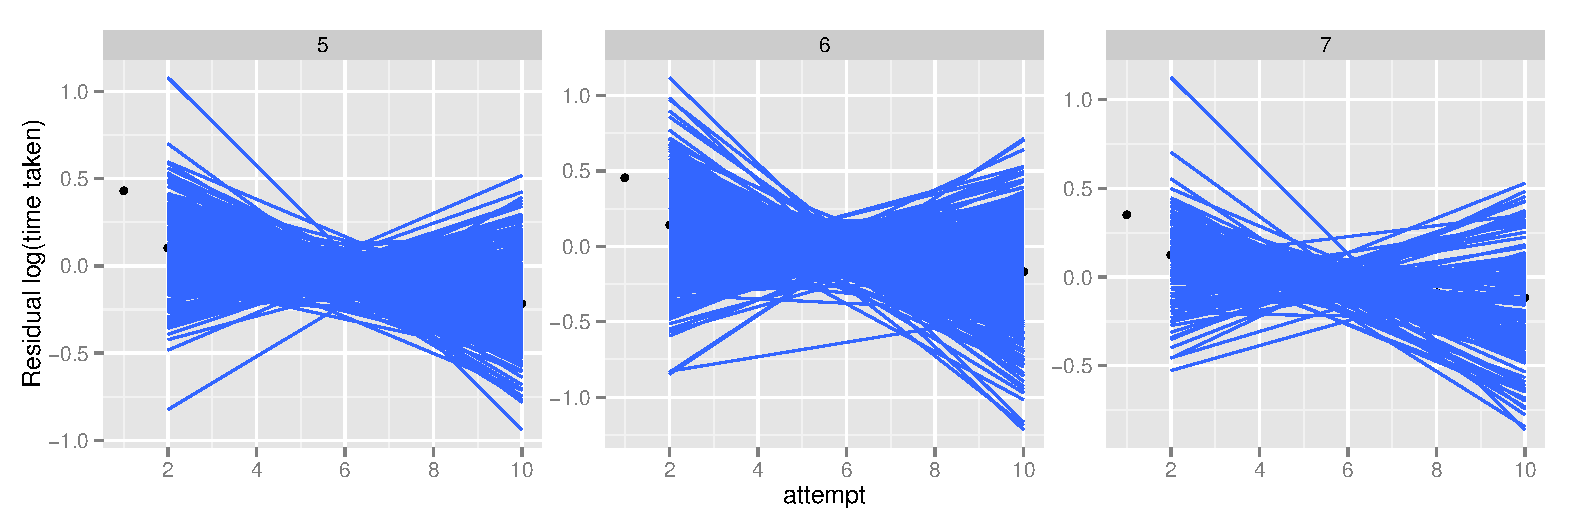
\includegraphics[width=6.3in]{learning_trend_time_subject.pdf}    
   \caption{Least square regression lines fitted through the subject specific residuals obtained by  fitting Model \eqref{eqn:trend_time} without covariate attempt. Differences in subject specific slopes are observed. Some of the subjects did worse over successive attempts while others did better. Averages of these residuals are plotted as dots and least square regression lines are fitted to obtain overall trends. For all the three experiments the overall downward slopes are statistically significant which indicates that MTurk workers take less time as they progress through their attempts.}
   \label{fig:learning_trend_time}
\end{figure}

\subsection{Lineup Design}

\subsubsection{Sample of lineup}
\subsubsection{Sample of Null Plots}

\subsubsection{Location Effect}

A total of 111 subjects were recruited to evaluate lineups designed to investigate the location effect of the actual data plot in the lineup as described in Section~\ref{sec:location_design}. Each subject evaluated two lineups;  one for Interaction effect and the other for Genotype.  In total there were 222 feedbacks or responses on 50 lineups. The data on the test lineup were excluded from the analysis.

The proportion of correct responses for each data plot location is shown in Figure \ref{fig:location_effect} colored by null sets. We observe some variability of performance for different null sets even though same data plot was used for all these null sets. This may happen when for some set of null plots, one null plot appears to be very similar to the actual plot. In another set of null plots this may not happen making some lineups easier than others even though the actual data plot is the same. This pattern is evident in the figure as we see proportion correct for null plot 5 is consistently above the null plot 1 for each of the locations. A test for differences in average performances of null sets shows significant difference only for null set 3 of interaction lineup. The rest of the null sets don't show any differences at 1\% significance level. 

\begin{figure}[htbp] 
   \centering
    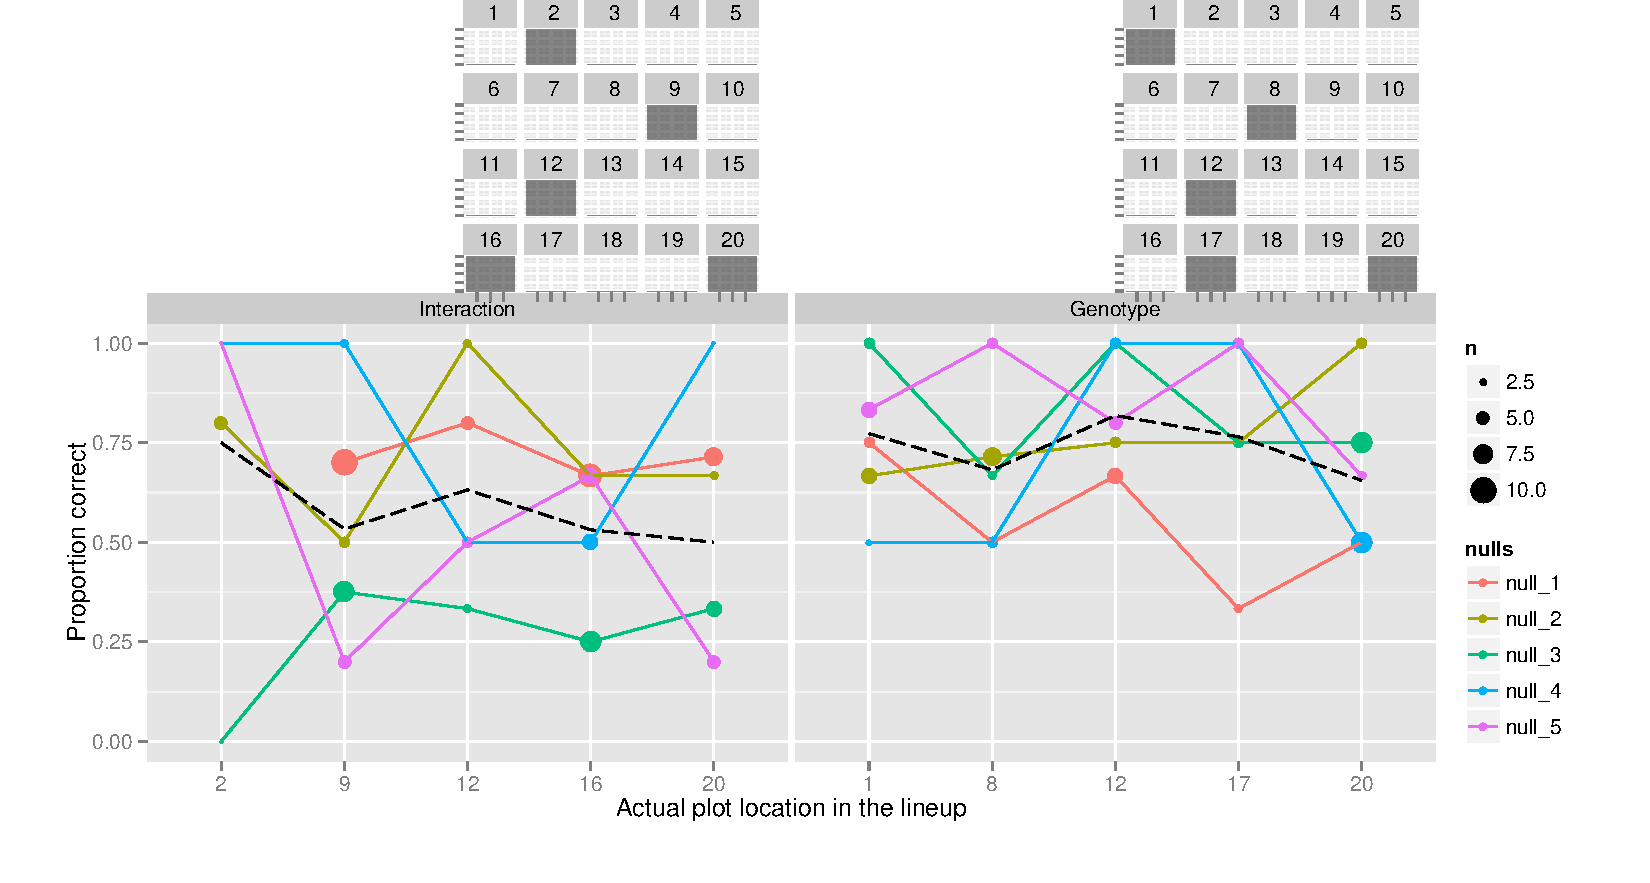
\includegraphics[width=6.5in]{proportion_nulls_guide.pdf} 
   \caption{Location of data plot in the lineup and proportion correct for both Interaction and Genotype effect. Each colored line represents a null set and the size of the dots represents number of responses. The overall average proportions are shown by dashed line. The actual data plot locations are shaded grey on the top panels to demonstrate their relative positions on a lineup.}
   \label{fig:location_effect}
\end{figure}

The overall average proportion of correct responses for each location are shown using dashed lines in Figure \ref{fig:location_effect}. There is variability in performances for each null set depending on the locations. But the overall proportion is not varying much for different locations. 

The sizes of the dots in  Figure \ref{fig:location_effect} represents the number of responses obtained for that location and null set. For some locations we have as many as 10 responses. For location 1, we did not have any response for null set 1 in one of the interaction lineups. We observe larger variability for interaction lineups as compared to Genotype lineups. It is because some of the interaction lineups were evaluated only once as we see for null plot 3 and 5 for Interaction effect. This leads to the extreme proportion of correct since one response will either be correct or wrong. The larger variability observed for Interaction lineups can be controlled at some extent by evaluating them multiple times.


We fitted Model \eqref{manova} to test if the mean performance vectors are similar for different locations. For this we use {\it anova()} function of {\it stats} package of \cite{R:2012}. The results are shown in Table \ref{tbl:manova}. The $p$-values for both Interaction and Genotype effect are much bigger than the conventional threshold of 0.05. This suggest that there may be no difference in location. 

\begin{table}[hbtp]
\caption{The results obtained by fitting MANOVA Model \eqref{manova}.}
\begin{center}
\begin{tabular}{ccccccccc}
  \hline \hline
 Location & && & \multicolumn{3}{c} {Degrees of Freedom}  & F test \\
 \cline{5-7}
 Effect & DF & Pillai & Approx. F & Numerator& Denumerator &Residual & $p$-value\\
  \hline
  Interaction& 3&1.4783 &0.7772&15&12 & 6 & 0.6821 \\ 
  Genotype &4&1.7796 &1.1221&20&28 & 8 &  0.3824 \\ 
   \hline
\end{tabular}
\end{center}
\label{tbl:manova}
\end{table}


We also examined whether the proportion of correct responses differs if the actual plot is on the outer boundary or in the inner locations. The locations 7,8,9,12,13,14 in the lineup are considered inner locations and the rest of the boundary locations are considered to be outer location. As we see in Figure \ref{fig:location_effect}, location 9, 12 are inside for Interaction effect and location 8, 12 are inside for Genotype. It does not show any differences whether the actual plot is inside or outer border of the lineup. We also fitted Model \eqref{manova} with two locations, inner and outer, as covariate and observed no significant differences. 



%
%% latex table generated in R 2.15.0 by xtable 1.7-0 package
%% Fri Sep  7 10:28:47 2012
%\begin{table}[hbtp]
%\caption{Fixed effect parameter estimates of generalized mixed model. Note that attempt is not significant for experiment 2. The continuous covariate, lineup difficulty, was measured by the $p$-value of the actual plot in the lineup.}
%\begin{center}
%\begin{tabular}{llrrrrl}
%  \hline
%& Parameters & Estimate & Std..Error & z.value & P-value  & \\ 
%  \hline
%\multicolumn{2}{l}{\bf{Experiment 1} } &&&& &\\
%&(Intercept) & -0.30 & 0.10 & -2.89 & 0.00 & ***\\ 
% & attempt & 0.08 & 0.02 & 4.21 & 0.00 & ***\\ 
% & lineup difficulty & -11.32 & 1.01 & -11.19 & 0.00 & ***\\ 
%\multicolumn{2}{l}{\bf{Experiment 2} } &&&&& \\
% & (Intercept) & 2.36 & 0.15 & 16.09 & 0.00 & ***\\ 
% & attempt & 0.01 & 0.03 & 0.35 & 0.72 \\ 
% & lineup difficulty & -55.03 & 2.20 & -25.00 & 0.00 & ***\\ 
%\multicolumn{2}{l}{\bf{Experiment 3} } &&&& \\
% & (Intercept) & 0.25 & 0.16 & 1.58 & 0.11 & .\\ 
% & attempt & 0.10 & 0.03 & 3.34 & 0.00 & ***\\ 
% & lineup difficulty & 3.00 & 0.56 & 5.36 & 0.00 & ***\\ 
%   \hline
%\end{tabular}
%\end{center}
%\label{tbl:model_par}
%\end{table}
%
% \footnote{Signif. codes: 0 �***� 0.001 �**� 0.01 �*� 0.05 �.� 0.1}




\section{Conclusion}

Human demographics have significant influence on performance in time taken to evaluate a lineup. Some variations among the factors are observed in terms of probability of correct evaluation. Age group 36-40, Countries other than India and United states, People who have a graduate degree are significantly different. But their practical impact on probability to correctly evaluate a lineup is very negligible and in some cases it diminishes  as the lineup difficulties increase or decrease. Gender does not have any significant effect on performance. Thus there may be differences in time taken to evaluate a lineup for different human demographics but the practical impact of demographics on the performance is very negligible. This result is very important for the power of visual test as it demonstrates the robustness of the test for different human factors.

Individual learning trend is observed in both time taken and observer performance. Some individuals improved the performances while others showed decrease in their performances over attempts. But the overall performance of the observers does not increase through successive attempts while evaluating multiple lineups. This result suggests that the power estimated for visual inference using human subject experiment is robust and may not change if those participants are allowed to give feedback again. The skill in evaluating the lineup in shorter time gets improved over successive evaluations. The earlier evaluations take significantly longer time than the later evaluations.  It suggests that the skilled person may only do it faster.

The simulation experiment reveals that there is no significant effect of location of actual data plot in the lineup. This is important as the visual statistical inference procedure suggests that the data plot be placed at random anywhere in the lineup. This paper suggests that any random place in a lineup is as good as other places in the lineup. Even though there are variations on the performance depending on different null sets, their impact on probability to correctly evaluate a lineup is very negligible.

The subjects participating this study may not necessarily know about statistical graphics. The numerous pilot studies done with more trained participants suggest that power of visual statical inference may be higher for observers who have advanced knowledge about statistical graphics. The fact that a person with graduate degree performs better may be associated with this. But a graduate degree does not necessarily mean to have training on statistical graphics. More experiments may be needed to learn about the differences in power with trained and a non-trained observer in terms of knowledge about statistical graphics. 

This investigation allowed each observer to evaluate 10 lineups assuming that it would not cause fatigue or disinterest toward the task of evaluating lineups. This assumption is made based on the pilot studies. The future research may involve doing more experiments to check if fewer or more than 10 lineups have any significant impact on performance of the observer. The learning trend in terms of time taken shows downward trends. At some point it should level of. It will be useful to know for how many lineups time taken levels off to decide how many lineups is appropriate to show.

A lineup with fewer or larger than 20 plots may yield different results. If the size of the lineup is much higher than 20, it is intuitive that there may be location effect of the data plot in the lineup. It is because, the observer may get tired of scanning and may make decision based on the partial scanning of the lineup. On the other hand fewer than 20 plots will allow observer to compare the actual plot with fewer null plots giving more chance of picking actual plot as an error not as an actual plot. These are the some of the issues that require further investigation.


%------------------------------------------------------------------------------------
\paragraph{Acknowledgments}
%------------------------------------------------------------------------------------
This work was funded in part by National Science Foundation grant DMS 1007697. All studies were conducted with approval from the Institutional Review Board IRB 10-347.


\section{Some Figures and Tables (May go to Appendix)}

\subsection{How People Pick the Data Plot} In each of the experiments observers were asked to choose the reason for their selection of a particular data plot. \cite{majumder:2013} showed that these choice reasons may provide the clue on how people picks the data plot in the lineup. To investigate this further we added free text input option in experiment 9 for their choice reason instead of some fixed reasons to select from. This allowed observers to write whatever they think their reasons for choice are. Figure \ref{fig:wordle} shows the words used to explain their reasons for choice. The most common words used to explain their choice are points and green which indicates the use of two important features of the grammar of graphics \citep{wilkinson:1999, hadley:2009}. One is the indicator of geometric shape and the other is the aesthetics. Spread, steepest, line and apart are some other important words used frequently. Spread and apart are indicative of variability in the data. Steepest and line indicates some sort of systematic pattern in the data.


\begin{figure}[htbp] 
   \centering
   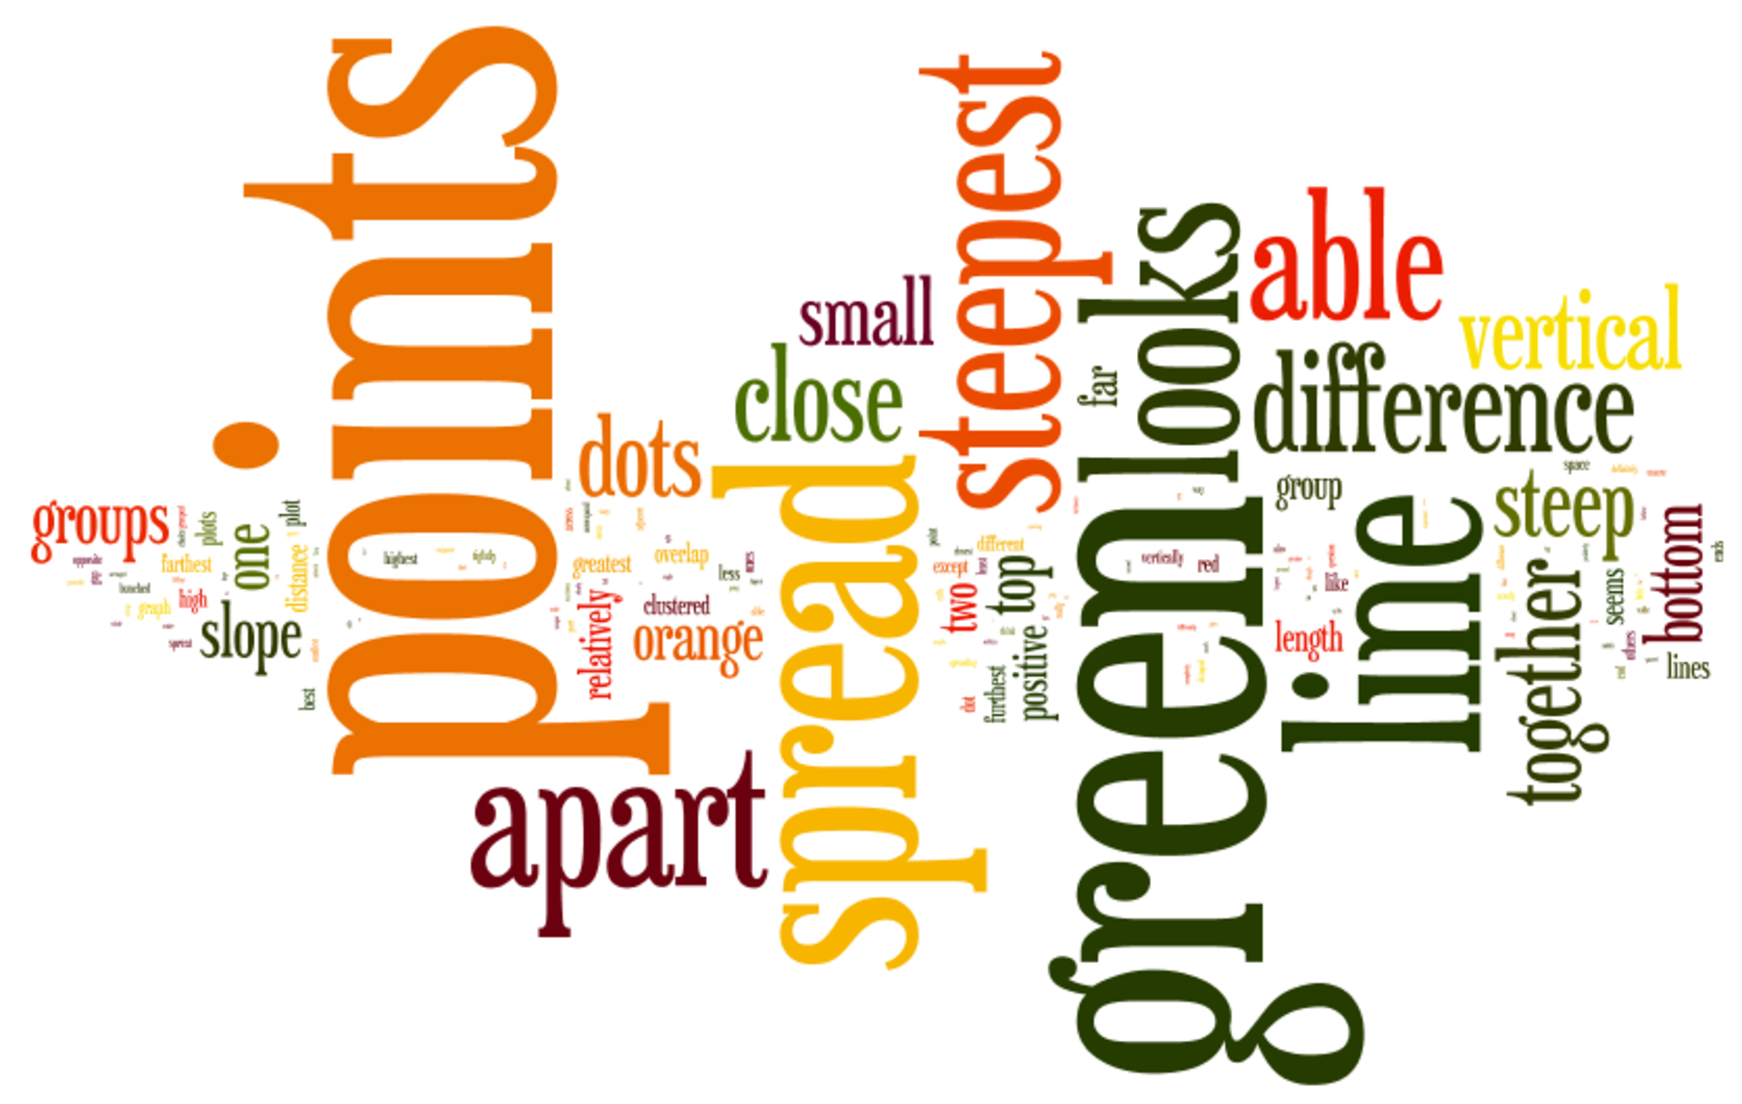
\includegraphics[width=3.5in]{reasoning_words.pdf} 
   \caption{Words used to explain the reasons for selection of data plot in a lineup show what features of a lineup may help a non-statistician to evaluate it. Larger font indicate more people choosing that word. Different color is used just to separate the words.}
   \label{fig:wordle}
\end{figure}

Figure \ref {fig:wordle} also shows some insight about peoples way of reading a plot. We notice that variability in the data, geometric shapes and aesthetics used to generate plots and existence of any systematic pattern in the plot are some of the important features revealed from the figure. These features are commonly used by human brain to examine and compare plots. Notice that these features may be specific to this particular experiment. There can be different other features people may use to evaluate a lineup depending on the situation. But with these words we get a general idea on how people may think while evaluating a lineup.

Turk workers are not necessarily trained on statistics or aware of specific terms used in statistics or statistical plots let alone having knowledge about grammar of graphics. It is interesting that people explain things that have specific definitions and meaning in the literature. For example, some keywords like spread, apart should be analogous to larger variability while together,  close may be for indicating smaller variability. Thus the perception from a statistical graphics is intuitive and human intelligence learn this even without having specific training. This is why visual inference can be used as a tool for teaching inference in the basic statistics classes.


%\begin{table}[hbtp]
%\caption{Amazon mechanical turk experiments and their properties. Duration in hours per 100 tasks show the popularity of some tasks compared to others.}
%\centering
%\begin{tabular}{rlrrrrrrr}
%  \hline
%& Experiment& \multicolumn{2}{c}{ Total Task}& Average & \multicolumn{2}{c}{Duration (hour)} & Payment & Pay rate\\
%\cline{3-4} \cline{6-7}
%Serial & description & submitted & rejected & time(min) & Actual & 100 task& \$/task & \$/hour\\ 
%  \hline
%1 & Boxplot & 406 & 106 & 10.68 & 146.48 & 36.08 & 0.50 & 2.81 \\ 
%  2 & Scatterplot & 359 &   9 & 10.80 & 42.68 & 11.89 & 1.00 & 5.58 \\ 
%  3 & Contaminated plot & 219 &  19 & 13.53 & 126.17 & 57.61 & 1.00 & 2.22 \\ 
%  4 & Polar vs Cartesian & 110 &  10 & 20.65 & 11.65 & 10.59 & 1.00 & 2.91 \\ 
%  5 & Hist vs density & 234 &  37 & 17.85 & 41.57 & 17.76 & 1.00 & 3.36 \\ 
%  6 & Violin vs boxplot & 417 &  17 & 17.95 & 105.87 & 25.39 & 1.00 & 3.34 \\ 
%  7 & Group separation & 106 &   6 & 16.13 & 5.15 & 4.86 & 1.00 & 3.72 \\ 
%  8 & Sine Illusion & 101 &   1 & 16.52 & 78.38 & 77.60 & 1.00 & 3.63 \\ 
%  9 & Gene expression & 103 &   3 & 12.47 & 11.27 & 10.94 & 0.50 & 2.41 \\ 
%  10 & Test normality & 406 &   6 & 22.70 & 74.35 & 18.31 & 1.00 & 2.64 \\ 
%   \hline
%\end{tabular}
%\label{tbl:mturk}
%\end{table}
%
%
%\begin{figure}[htbp] 
%   \centering
%   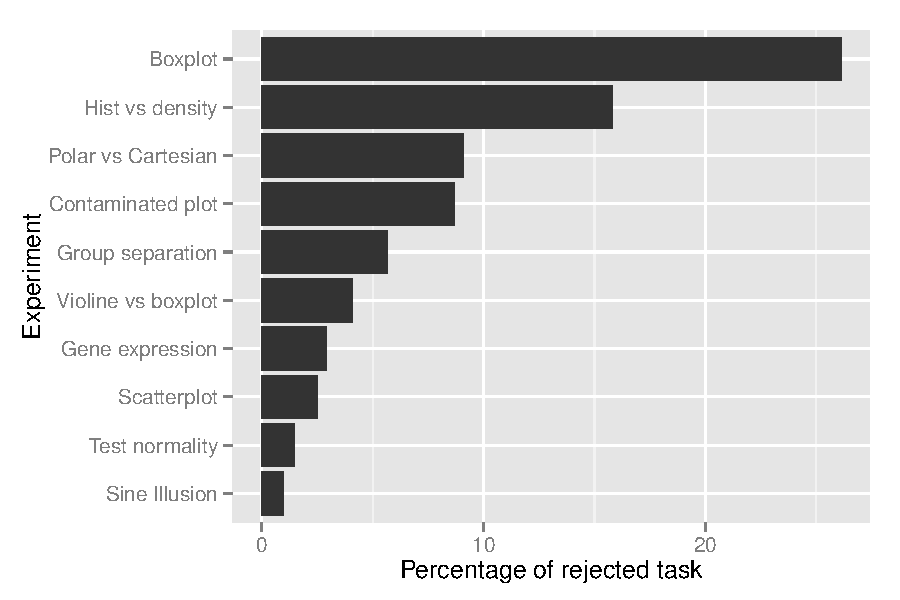
\includegraphics[width=3in]{rejected_task.pdf}
%      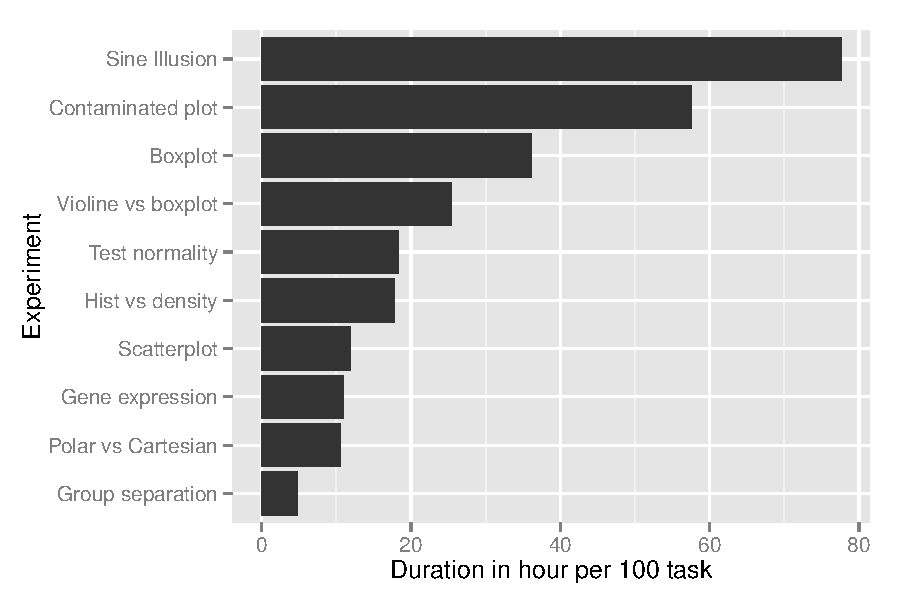
\includegraphics[width=3in]{task_duration.pdf} 
%   \caption{Percentage of rejected tasks and duration of each experiment in hour per 100 tasks for each of the 10 experiments. Most of the tasks got rejected for box plot experiment.  Even though the sine illusion experiment took longest to finish the rejection rate is lowest for this experiment.}
%   \label{fig:task_duration}
%\end{figure}




%\clearpage
\section{Some Plots of Exploratory Data Analysis}

This section includes some plots showing results from exploratory data analysis. The results are discussed in Section~\ref{sec:result_socio}.

\begin{figure}[htbp] 
   \centering
   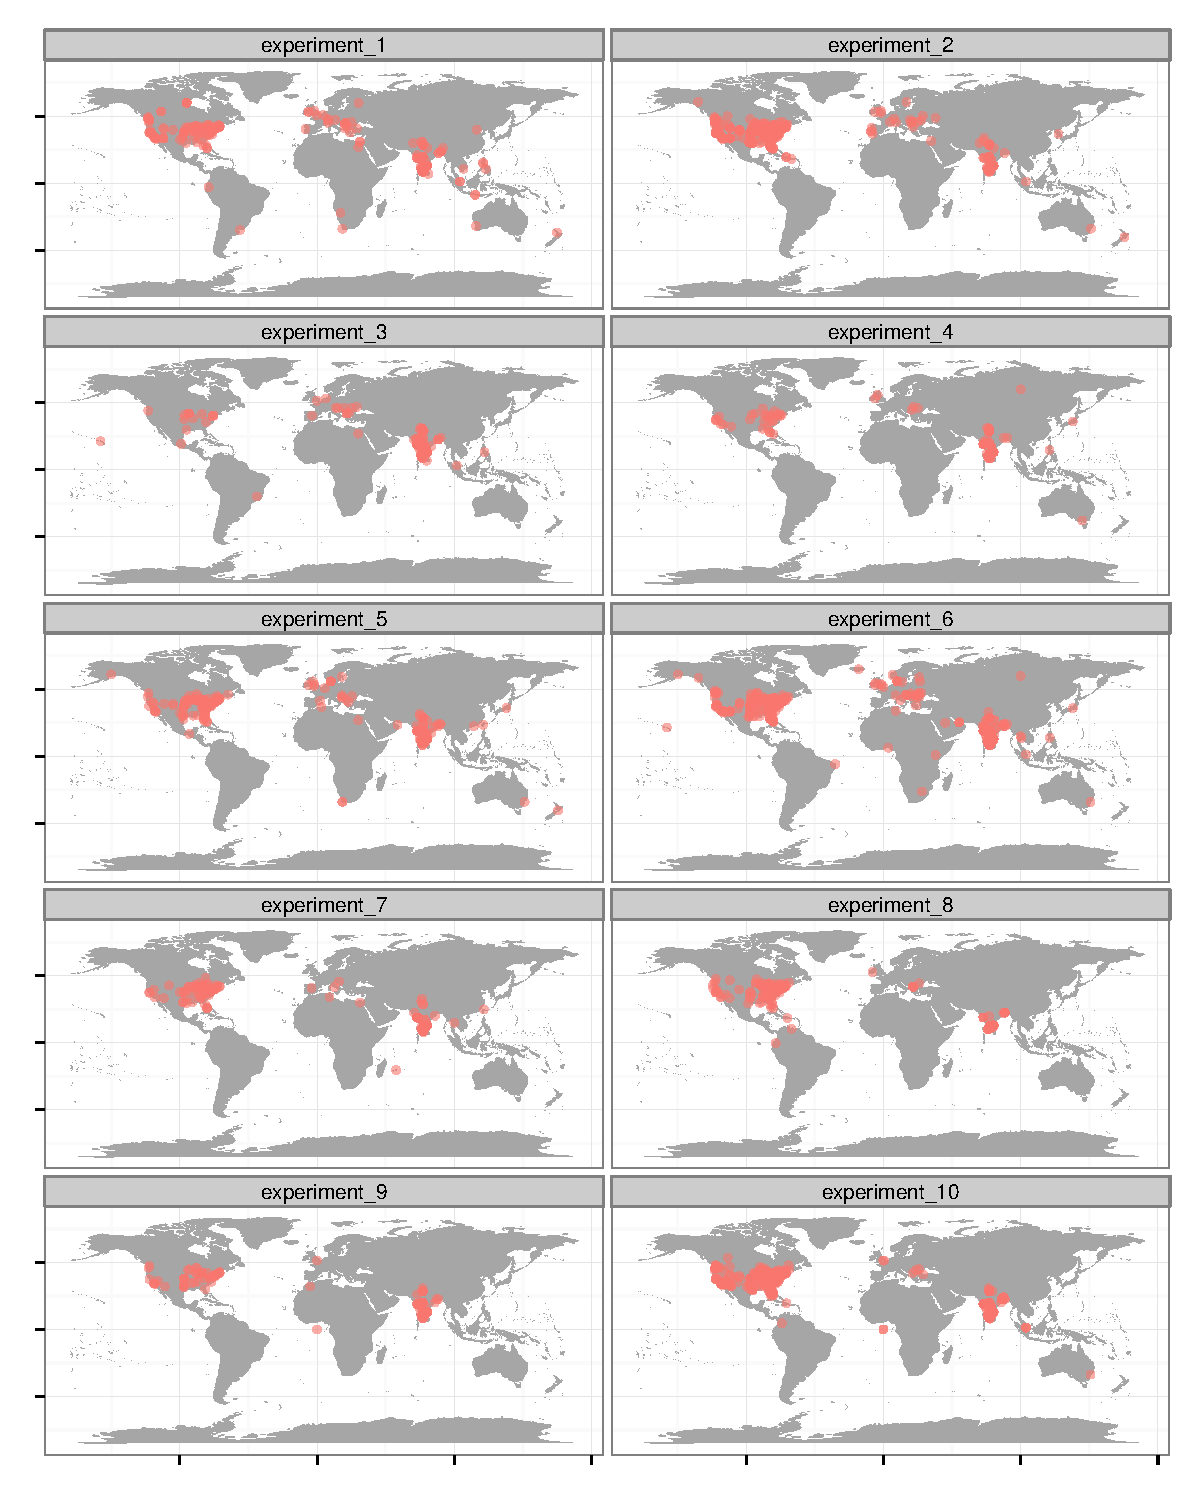
\includegraphics[width=5.8in]{turker_location_experiment.pdf} 
   \caption{World maps showing where the participants are coming from for all the 10 experiments.}
   \label{fig:turker_location_experiment}
\end{figure}

\begin{figure}[htbp] 
   \centering
   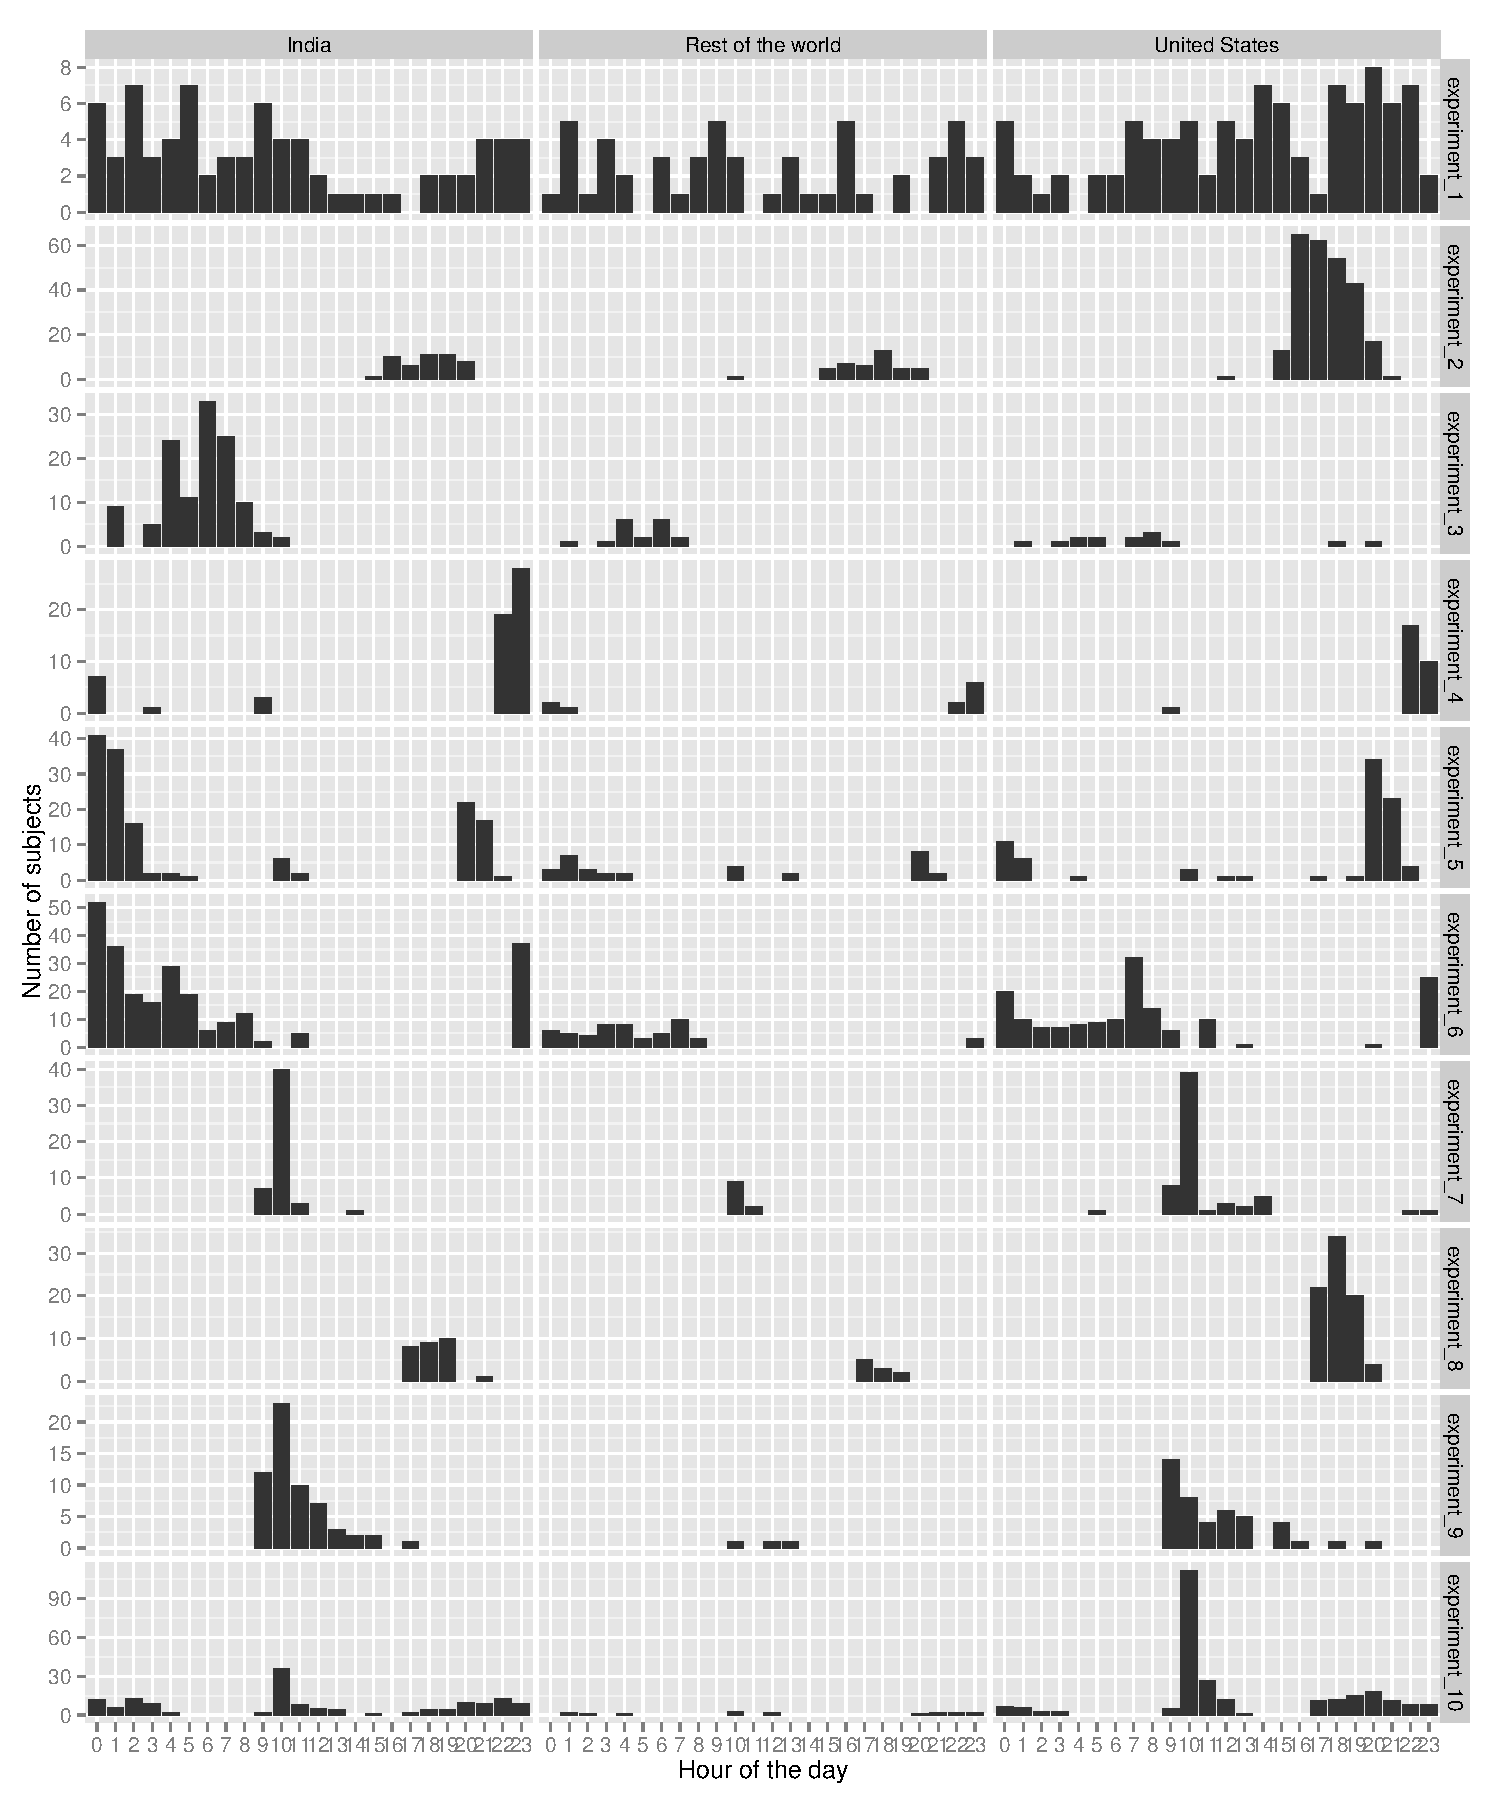
\includegraphics[width=6.5in]{participation_time.pdf} 
   \caption{Number of participants by time of the day feedbacks received (central time). Experiment 1 shows MTurk workers participated the experiments around the clock. Other experiments did not take a whole day to finish. For experiment 3 most of the participants are from India because of timing. No matter when the experiment is started, subjects from India shows participations. For United States, subjects participated if the experiment is not in the mid night, except for experiment 6.}
   \label{fig:participation_time}
\end{figure}



\begin{figure}[htbp] 
   \centering
   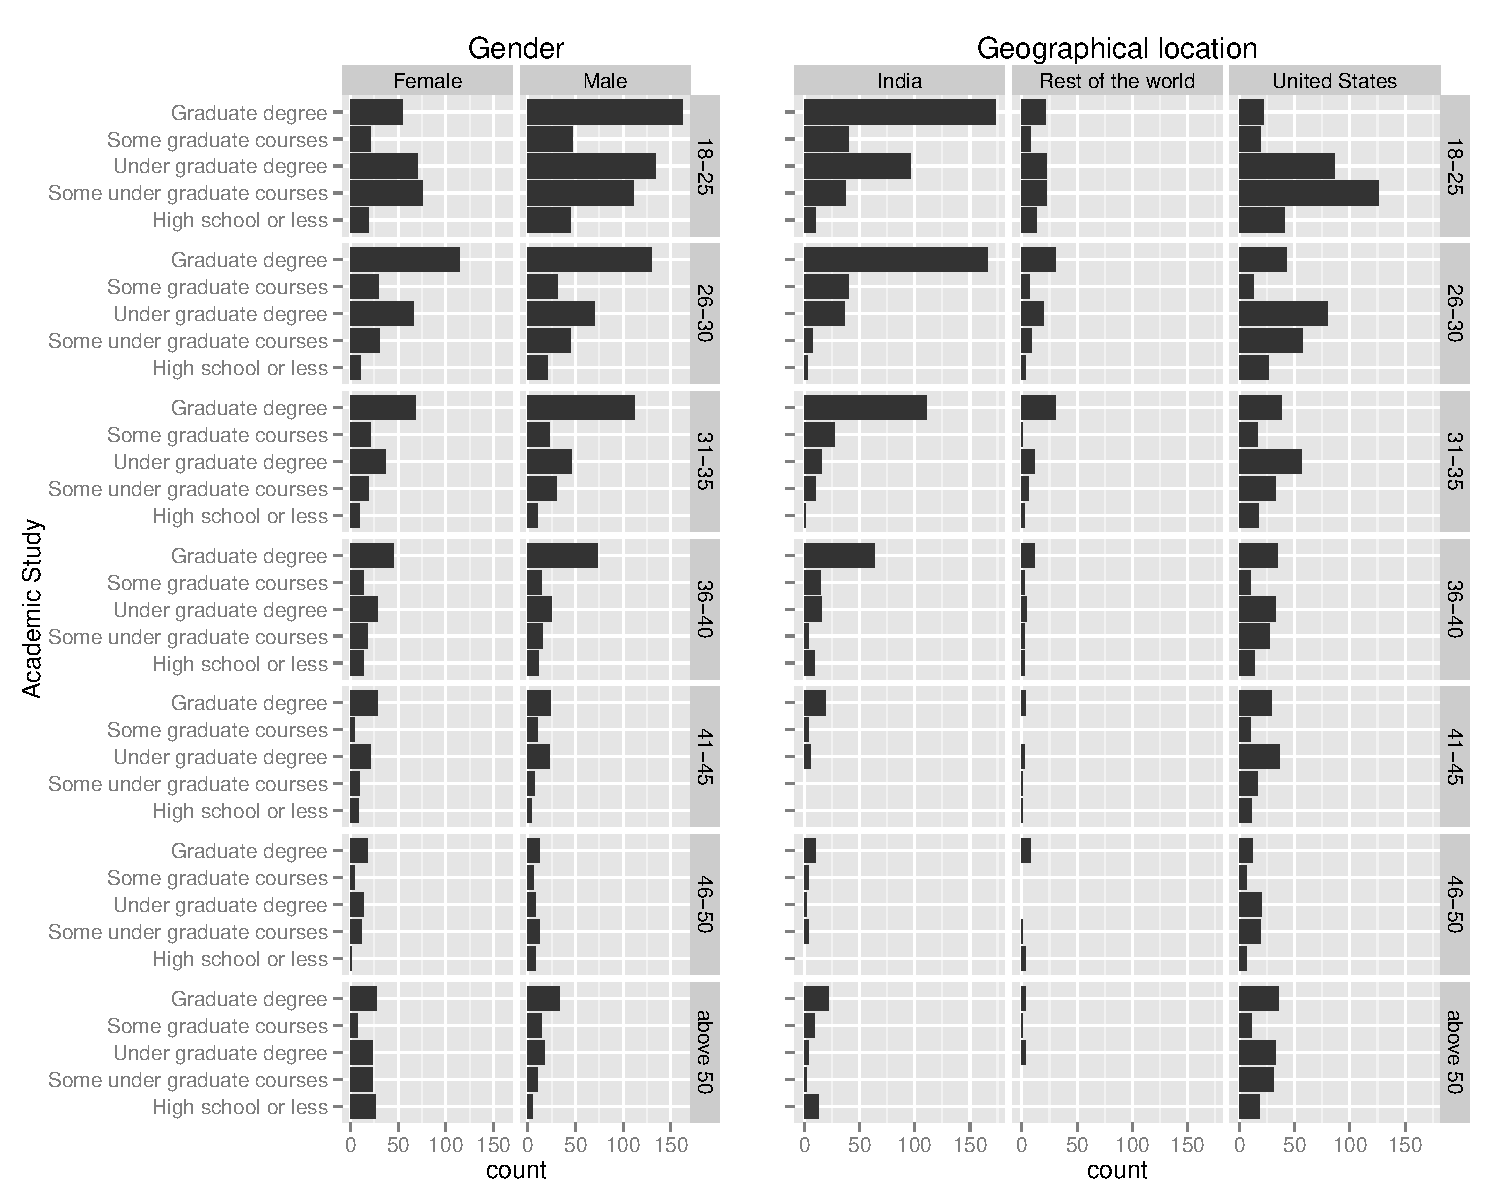
\includegraphics[width=6in]{demographic_info.pdf} 
   \caption{Countrywise distribution of age and academic levels of the MTurk workers participating the experiments shows the diversity of the subjects in all the demographic aspect. Almost equal number of male and female subjects participated the online experiments.}
   \label{fig:demographic_info}
\end{figure}


\begin{figure}[htbp] 
   \centering
   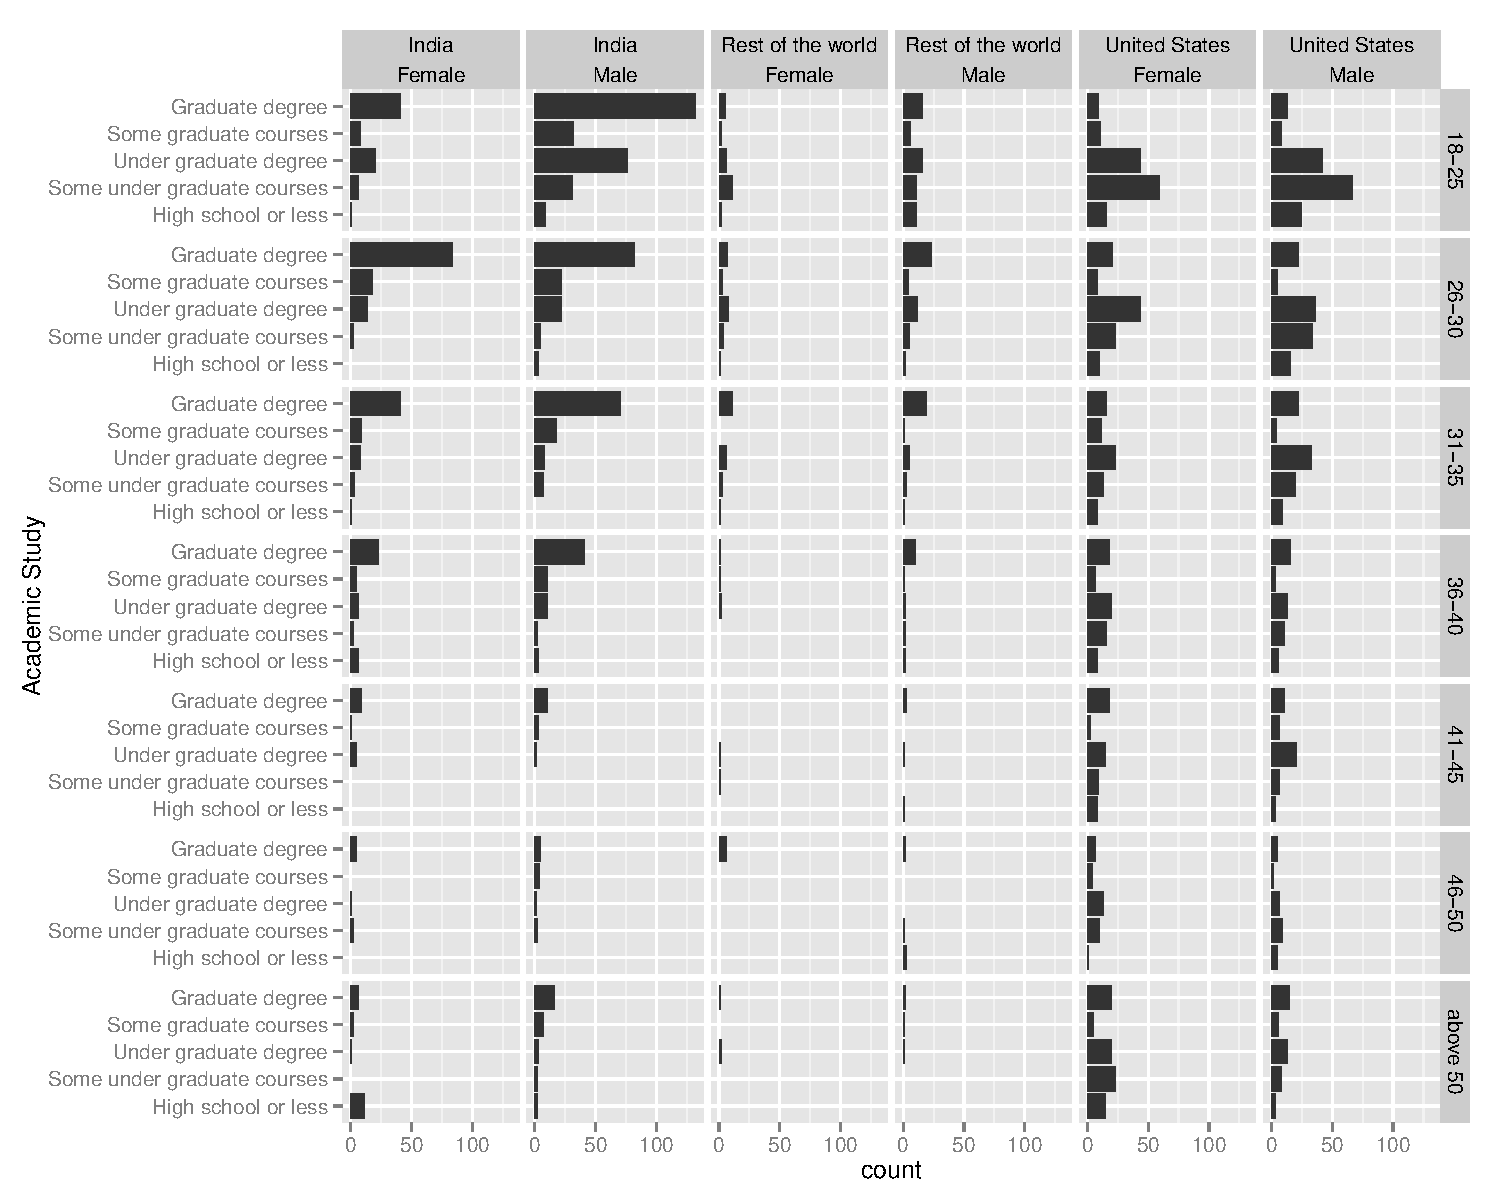
\includegraphics[width=6.5in]{age_gender_within_country_bar.pdf} 
   \caption{Countrywise distribution of age and academic levels of the MTurk workers participating the experiments shows the diversity of the subjects in all the demographic aspect. Male and female participants differ in India specially for agelevel 18-25. For United States number of participants are similar beyond age 40 while few number of participants coming from India beyond that age.}
   \label{fig:gender_country_bar}
\end{figure}


\begin{figure}[htbp] 
   \centering
   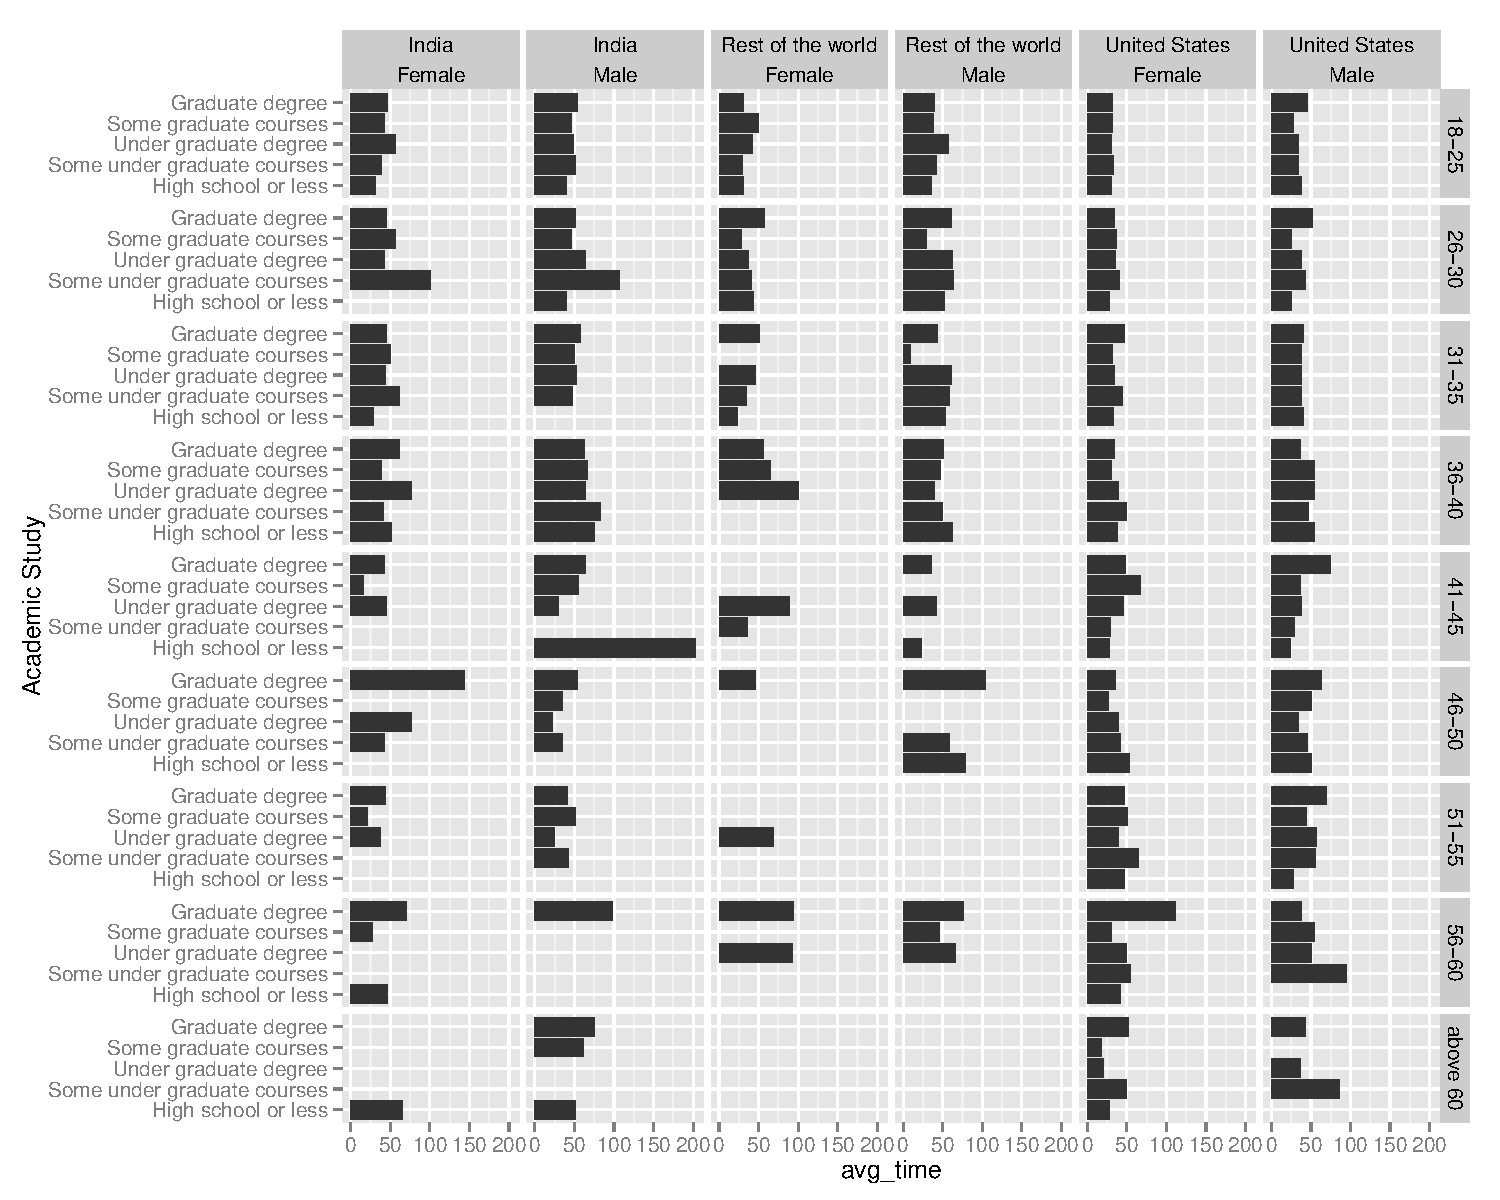
\includegraphics[width=6.5in]{age_gender_within_country_time.pdf} 
   \caption{Countrywise average time taken for different age and academic levels of the MTurk workers participating the experiments shows that the demographic factors may not have effect on time taken. }
   \label{fig:gender_country_time}
\end{figure}


\begin{figure}[htbp] 
   \centering
   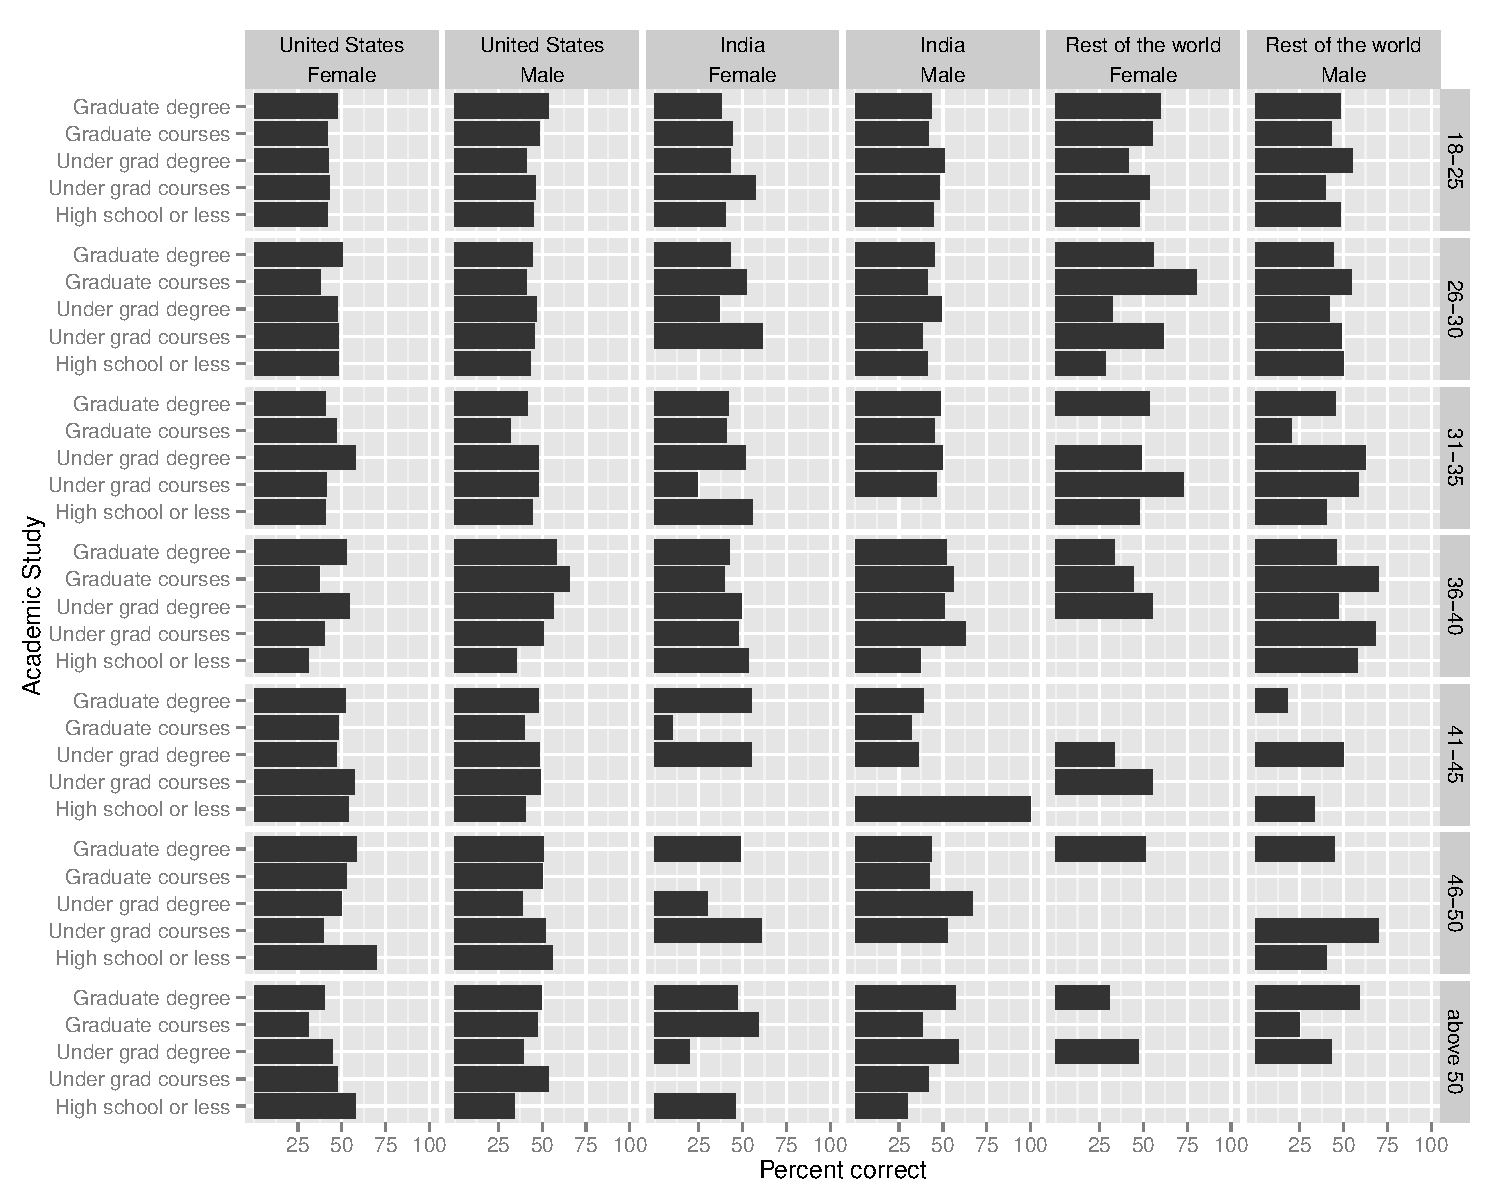
\includegraphics[width=6.5in]{age_gender_within_country_correct.pdf} 
   \caption{Countrywise percentage of correct responses for different age and academic levels of the MTurk workers participating the experiments shows that the demographic factors may not have effect on the percentage of correct responses. }
   \label{fig:gender_country_response}
\end{figure}





%\begin{figure}[htbp] 
%   \centering
%   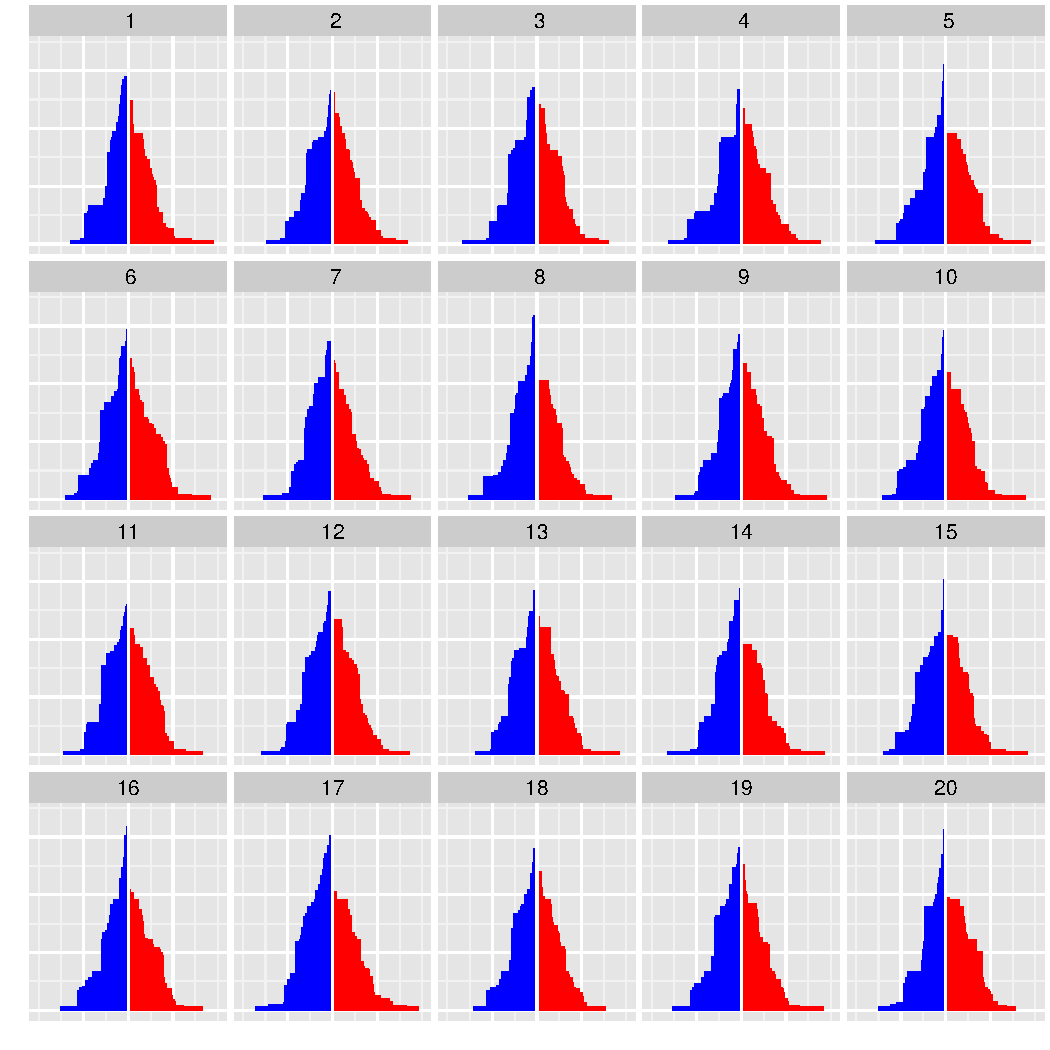
\includegraphics[width=0.8\linewidth]{electoral-2-17.pdf} 
%   \caption{Lineup \#2 - electoral building. Which building looks the most different from the other buildings? }
%   \label{fig:elect.2}
%\end{figure}
%\begin{figure}[htbp] 
%   \centering
%   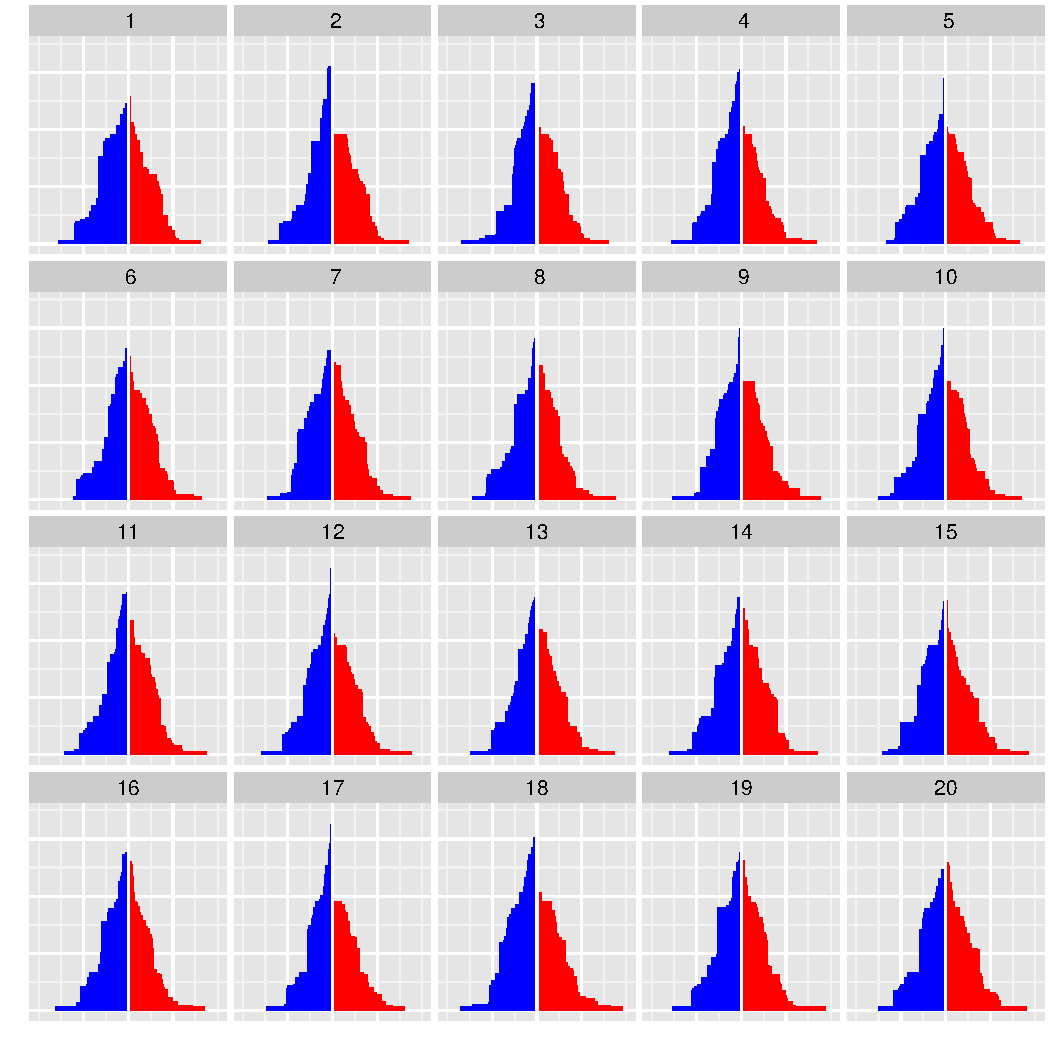
\includegraphics[width=0.8\linewidth]{electoral-3-18.pdf} 
%   \caption{Lineup \#3 - electoral building. Which building looks the most different from the other buildings? }
%   \label{fig:elect.3}
%\end{figure}
%\begin{figure}[htbp] 
%   \centering
%   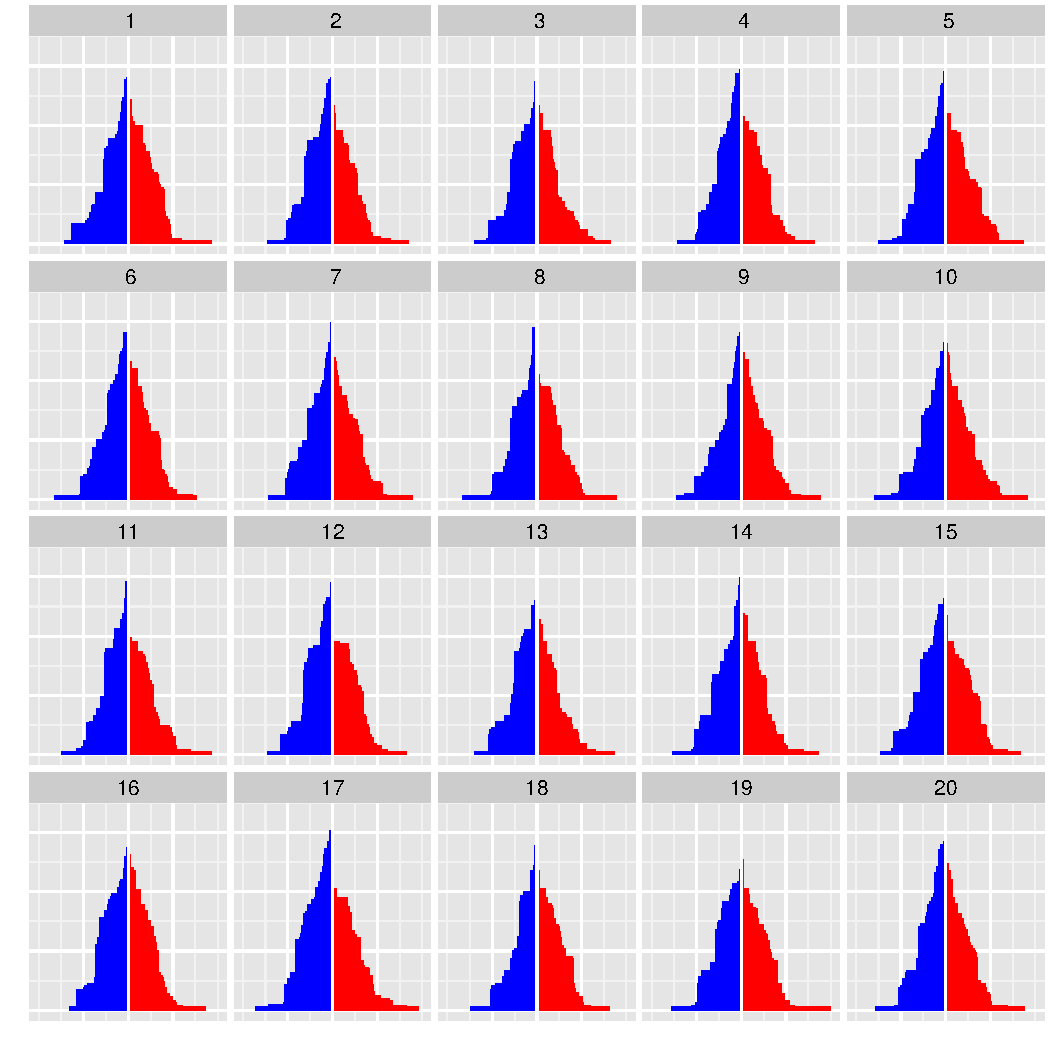
\includegraphics[width=0.8\linewidth]{electoral-4-17.pdf} 
%   \caption{Lineup \#4 - electoral building. Which building looks the most different from the other buildings? }
%   \label{fig:elect.4}
%\end{figure}
%\begin{figure}[htbp] 
%   \centering
%   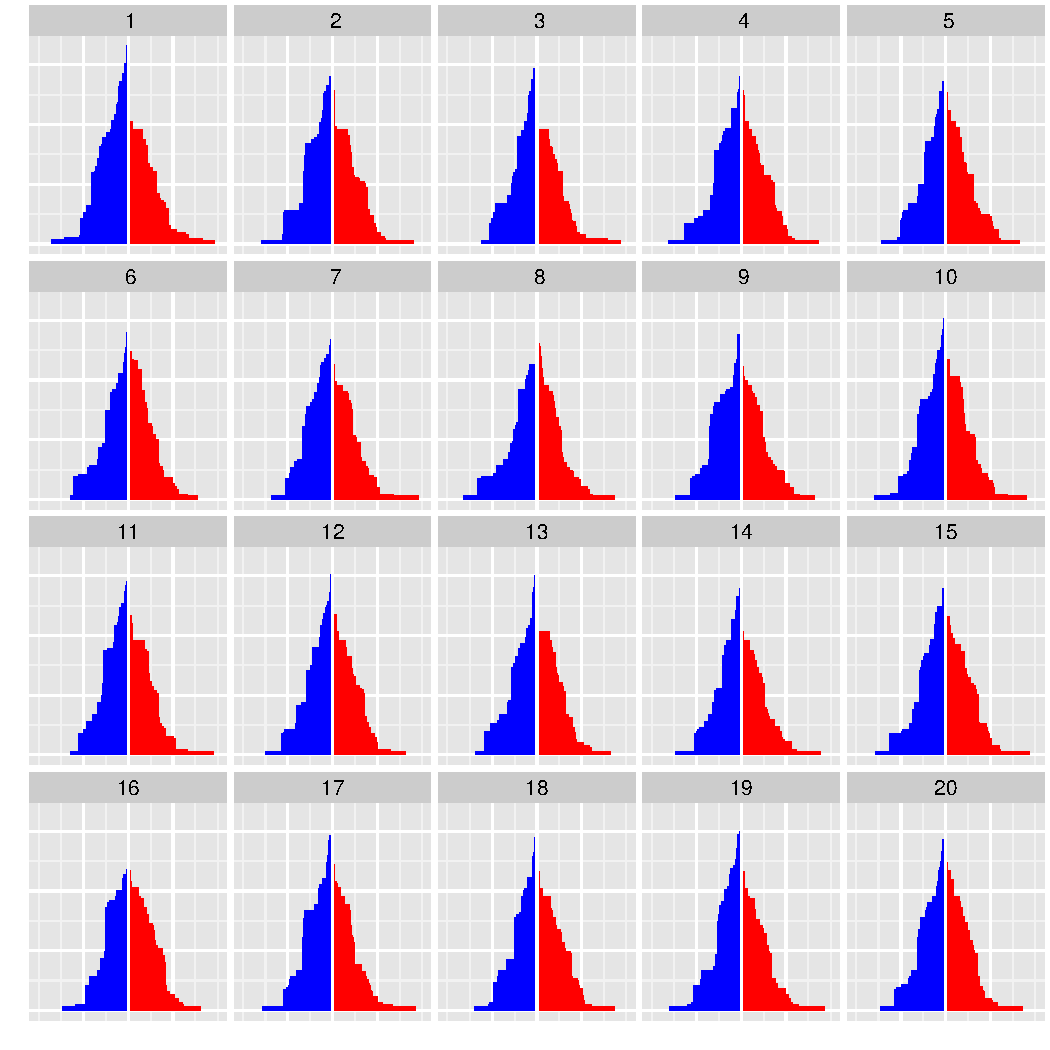
\includegraphics[width=0.8\linewidth]{electoral-1-1.pdf} 
%   \caption{Lineup \#5 - electoral building. Which building looks the most different from the other buildings? }
%   \label{fig:elect.5}
%\end{figure}


\clearpage
\section{Electoral Building Lineups and Results}
%Figures~\ref{fig:elect-1} and \ref{fig:elect.2} through~\ref{fig:elect.5}

Five lineups were shown to (different) Amazon Turk workers in an experiment. They all were created as described in the introduction of the paper. In order to not bias observers, no context information was given about how these plots were created or what data they were displaying. This also made it necessary to slightly more stylize the display. 

% latex table generated in R 3.0.1 by xtable 1.7-1 package
% Wed Jun  5 17:39:09 2013
\begin{table}[hbtp]
\centering
\begin{tabular}{rrrrrr}
  \hline
 lineup & \#1 & \#2 & \#3 & \#4 & \#5 \\ 
  \hline
  \# correct/ \#evaluation &  12/72 & 11/66 & 5/74 & 14/72 & 19/57 \\ 
$p$-value & 0.00023 & 0.00041 & 0.31 & 1.2e-05 &  1.9e-11 \\ 
data panel & $3\cdot4+1$ & $2^4+1$ & $4^2+2 $ & $12+\sqrt{25}$ & $2^3-7$ \\ 
   \hline
\end{tabular}
\end{table}

% latex table generated in R 3.0.1 by xtable 1.7-1 package
% Wed Jun  5 18:00:55 2013
\begin{table}[hbtp]
\centering
\caption{\label{tbl:response}Overview of all choices by observers for each of the lineups. The correct choice is bolded. In most lineups there are null plots that were picked more often by observers, but the actual result is among the plots being picked most often, indicating that there is some indication that the election result is not completely consistent with the polls.}
\scalebox{.9}{
\begin{tabular}{rrrrrrrrrrrrrrrrrrrrr}
  \hline
& \multicolumn{10}{l}{panel chosen}\\
Lineup & 1 & 2 & 3 & 4 & 5 & 6 & 7 & 8 & 9 & 10 & 11 & 12 & 13 & 14 & 15 & 16 & 17 & 18 & 19 & 20 \\ 
  \hline
\#  1 & 2 & 2 & 0 & 10 & 2 & 2 & 6 &  23 & 1 & 1 & 0 & 1 & \bf 12 & 3 & 3 & 1 & 0 & 1 & 1 & 1 \\ 
\#  2 & 0 & 16 & 1 & 1 & 5 & 1 & 0 & 8 & 0 & 2 & 0 & 0 & 0 & 4 & 2 & 1 & \bf 11 & 1 & 0 & 13 \\ 
\#  3 & 7 & 26 & 0 & 2 & 0 & 5 & 3 & 0 & 2 & 1 & 0 & 4 & 0 & 0 & 2 & 0 & 9 & \bf 5 & 0 & 6 \\ 
\#  4 & 0 & 0 & 0 & 2 & 0 & 0 & 0 & 3 & 1 & 10 & 2 & 18 & 1 & 0 & 4 & 2 &\bf 14 & 0 & 13 & 0 \\ 
\# 5 &\bf 19 & 1 & 4 & 1 & 0 & 1 & 0 & 12 & 0 & 0 & 0 & 4 & 1 & 0 & 0 & 12 & 1 & 1 & 0 & 0 \\ 
   \hline
\end{tabular}
}
\end{table}





\bibliographystyle{asa}
\bibliography{references}

\end{document}



